% mnras_template.tex 
%
% LaTeX template for creating an MNRAS paper
%
% v3.0 released 14 May 2015
% (version numbers match those of mnras.cls)
%
% Copyright (C) Royal Astronomical Society 2015
% Authors:
% Keith T. Smith (Royal Astronomical Society)

% Change log
%
% v3.0 May 2015
%    Renamed to match the new package name
%    Version number matches mnras.cls
%    A few minor tweaks to wording
% v1.0 September 2013
%    Beta testing only - never publicly released
%    First version: a simple (ish) template for creating an MNRAS paper

%%%%%%%%%%%%%%%%%%%%%%%%%%%%%%%%%%%%%%%%%%%%%%%%%%
% Basic setup. Most papers should leave these options alone.
\documentclass[fleqn,usenatbib]{mnras}

% MNRAS is set in Times font. If you don't have this installed (most LaTeX
% installations will be fine) or prefer the old Computer Modern fonts, comment
% out the following line
%\usepackage{newtxtext,newtxmath}
% Depending on your LaTeX fonts installation, you might get better results with one of these:
\usepackage{mathptmx}
\usepackage{txfonts}
\usepackage[T1]{fontenc}

% Allow "Thomas van Noord" and "Simon de Laguarde" and alike to be sorted by "N" and "L" etc. in the bibliography.
% Write the name in the bibliography as "\VAN{Noord}{Van}{van} Noord, Thomas"
\DeclareRobustCommand{\VAN}[3]{#2}
\let\VANthebibliography\thebibliography
\def\thebibliography{\DeclareRobustCommand{\VAN}[3]{##3}\VANthebibliography}

\usepackage{graphicx}	% Including figure files
\usepackage{amsmath}	% Advanced maths commands
\usepackage{amssymb}	% Extra maths symbols


%%%%%%%%%%%%%%%%%%%%%%%%%%%%%%%%%%%%%%%%%%%%%%%%%%

%%%%% AUTHORS - PLACE YOUR OWN COMMANDS HERE %%%%%

% Please keep new commands to a minimum, and use \newcommand not \def to avoid
% overwriting existing commands. Example:
%\newcommand{\pcm}{\,cm$^{-2}$}	% per cm-squared

%%%%%%%%%%%%%%%%%%%%%%%%%%%%%%%%%%%%%%%%%%%%%%%%%%

%%%%%%%%%%%%%%%%%%% TITLE PAGE %%%%%%%%%%%%%%%%%%%

% Title of the paper, and the short title which is used in the headers.
% Keep the title short and informative.
\title[S-PLUS: Emission line objects]{Photometric identification of emission line sources in the southern photometric local Universe survey (S-PLUS)}

% The list of authors, and the short list which is used in the headers.
% If you need two or more lines of authors, add an extra line using \newauthor
\author[Guti\'{e}rrez-Soto et al.]{
L. A. Guti\'{e}rrez-Soto,$^{1}$\thanks{E-mail: gsoto.angel@gmail.com}
Second  Author,$^{2}$
Third Author$^{2,3}$
and Fourth Author$^{3}$
\\
% List of institutions
$^{1}$Departamento de Astronomia, IAG, Universidade de S\~{o}a Paulo, Rua do Mata\~{o}, 1226, 05509-900, S\~{o}a Paulo, Brazil\\
$^{2}$Department, Institution, Street Address, City Postal Code, Country\\
$^{3}$Another Department, Different Institution, Street Address, City Postal Code, Country
}

% These dates will be filled out by the publisher
\date{Accepted XXX. Received YYY; in original form ZZZ}

% Enter the current year, for the copyright statements etc.
\pubyear{2021}

% Don't change these lines
\begin{document}
\label{firstpage}
\pagerange{\pageref{firstpage}--\pageref{lastpage}}
\maketitle

% Abstract of the paper
\begin{abstract}
The emission line objects are very important objects in astronomy because reflects different class of objects that evolved physical mechanics that given counts of formation stellar process, presences the gas, shocks, star-burst in galaxies, the finals stage of stars among others process 
\end{abstract}

% Select between one and six entries from the list of approved keywords.
% Don't make up new ones.
\begin{keywords}
keyword1 -- keyword2 -- keyword3
\end{keywords}

%%%%%%%%%%%%%%%%%%%%%%%%%%%%%%%%%%%%%%%%%%%%%%%%%%

%%%%%%%%%%%%%%%%% BODY OF PAPER %%%%%%%%%%%%%%%%%%

\section{Introduction}

The existence of an ionizing radiation field can lead to Balmer hydrogen emission lines. From the presence  of the H Balmer lines in the optical spectra of some sources it is well known the possible presence of ionized gas. Many important astronomical objects involve the physics of photo-ionized gases and the interpretation of the emission-line spectra. Emission line objects as the H II regions allow us to study the star formation history of the far reaches of our Galaxy and of distant galaxies. Planetary nebulae let us to see the remaining envelope of dying stars. Star-burst galaxies and QSOs are one the most luminous objects and hence the most distant that can be observed. Their spectra can reveal details about of the first generation of star and the formation of heavy elements in the young universe. On the other hand, emission lines can also infer the presence or lack the accretion discs \citep{Schwope:2000, Ratti:2012}, the properties of single or double picked line can allow us to infer geometrical characteristics \citep{Horne:1986}, the nature of  donor stars in binary system \citep{Steeghs:2002, Spaandonk:2010, Casares:2015} and the compact objects as black holes \citep{Casares:2016}. 

Emission lines are also associated with stars in very early-type and/or very late evolutionary stage which are short phase. As already mentioned are also associated with binaries that experiencing mass transfer. These group of emission line stars includes young stellar (YSOs) and Herbig-Haro (HH) objects, post-asymptotic and some asymptotic giant branch (AGB), some red giant stars (RGB), Wolf-Rayet (WR) stars, supernova remnants, classical Be stars, active late-type dwarfs, interacting binary system like symbiotic stars (SySt) and cataclysmic variables (CV). Most of these class of object are in-homogeneous and some contains many few identified members, for instance at the moment around 323 symbiotic system have been identified from which 257 belong to the Galaxy and  $\sim$66 are extra-galactic objects \citep{Akras:2019a}. The same occurs with PNe from witch around 3500 of them are been cataloged \citep{Parker:2016}, this current number of PNe represents only about 15-30\% of the estimated total of Galactic PNe (Frew, 2008; Jacoby et al., 2010) showing that a small fraction of the PNe have been cataloged. Many galaxies, in addition to harbor Planetary nebulae and H II regions, show characteristic nebular in their spectra. In most of these objects, the gas is photoionized by hot stars in the nucleus, which is thus much like giant H II region, or perhaps many H II regions. The galactic nucleus with very strongest  emission lines of this type are often called blue compact galaxies, extragaltic H II regions, star forming or starburst galaxies \citep{Osterbrock:2006}. There are also spiral galaxies that present emission lines.

In the past H$\lpha$ surveys with modest spatial resolutions have been used to identified extended nebular emission to study supernova remnants, galaxy groups and star forming regions (Davies, Elliott & Meaburn 1976). More recently, higher resolution surveys such as the INT Photometric H$\alpha$ survey (IPHAS; \citealt{Drew:2005, Barentsen:2014}) have focused in the study of compact emission line sources on the Galactic plane, typically with objects in different stage of stellar evolution. The Anglo-Australian Observatory UKS chmidt Telescope Supercosmos H$\alpha$ Survey (Parker et al. 2005) is anothe H{$\alpha$} survey of the Southern Galactic Plane and Magellanic Cloud which has covered to b $\sim$ 10-13$^{\circ}$ (verificar esto). Currently ongoing is the VST Photometric H$\alpha$ Survey of the Southern Galactic Plane and Bulge (VPHAS+; \citealt{Drew:2014}) that will cover the Galactic bulge and plane in five filters. 

Like VPHAS+, others ongoing surveys that are used to study the population of emission line objects are the The Javalambre Photometric Local Universe Survey (J-PLUS\footnote{\url{https://www.j-plus.es}}, \citealp{Cenarro:2018}) and the Southern-Photometric Local Universe Survey (S-PLUS\footnote{\url{http://www.splus.iag.usp.br}}, \citealp{Mendes:2019}) are providing observations of the Galactic halo covering both northern and southern celestial hemispheres in a systematic way with twin telescopes using the same set of multi-band filters. In addition to the H$\alpha$ filter, which is already vastly applied to systematically searching for H$\alpha$ emitters the telescopes offer 11 more filters. And more ambitious yet the JPAS survey that will the same area of J-PLUS in 56 narrow-band filters.

Traditionally, color-color diagrams based in H$\alpha$ filter are been used to identify H$\alpha$ emitters.  The analysis the color-color diagram  (r - H$\alpha$) versus (r - i) has resulted on the discoveried of new emission line objects, for instance \citet{Witham:2006, Witham:2007}  used the (r - H$\alpha$) versus (r - i) colour-colour diagram to find for new CV. On the other hand, \citet{Vink:2008} reported the discovery of YSOs by using this same colour criteria. In this sense using this methology a variety of classes of objects are been identified, which include symbiotic stars \citep{Corradi:2008, Corradi:2010, Corradi:2011}, early type emission line stars \citep{Drew:2008} and planetary nebulae \citep{Viirone:2009, Sabin:2010}. Recently, by using this same color diagram were also identified compact PN candidates in VPHAS+ catalog \citep{Akras:2019}. And the same diagram in conjunction with new ones shows to be very efficient to find for PN candidates \citep{Gutierrez:2020}. In general terms, \citet{Witham:2006} presented a methodology and first results in looking for emission line sources in narrow-band surveys.     

In this work, we used S-PLUS observations of the southern hemisphere to search for objects with an excess of H{$\alpha$} using automatic methods based on the (r - H$\alpha$) versus (r - i) color-color diagram we also used color criteria based in (g - r) and (z - g) in conjunction to unsupervised machine learning techniques to split the final list in those with blue and red continuum. The paper is organized as follows...

\section{Observations}
\label{sec:obser}

Particularly, we are implemented data from S-PLUS DR3 (ref) to carried out our study. S-PLUS is 12-band optical photometric survey, which are formed by using seven narrow-band and five brow-band like SDSS filters. The narrow-band set include the filter $J$0660 which detect the H{$\alpha$} emission line. Figure~\ref{fig:curves} shows the Javalambre filter system (Marín-Franch et al. 2012) overlapping are the optical spectra of several class emission line objects on which it is possible to see that the H{$\alpha$} line falls into the $J$0660 filter, except for the QSOs.   

The actual data release contains about 60 millions of objects covering a total area of $\sim$8000 deg$^2$, at high Galactic latitudes ($ > 30$~deg) using a dedicated 0.83m robotic telescope,the T80-South (T80S), located at Cerro Tololo, Chile. S-PLUS willcover an additional1300 deg2of the Galactic plane and bulge toenable Galactic studies. In this work, we focus on the aspects thatare of particular interest to the second data release of the S-PLUS main survey. Additional information about S-PLUS can be found in \citet{Mendes:2019}. 

\begin{figure}
    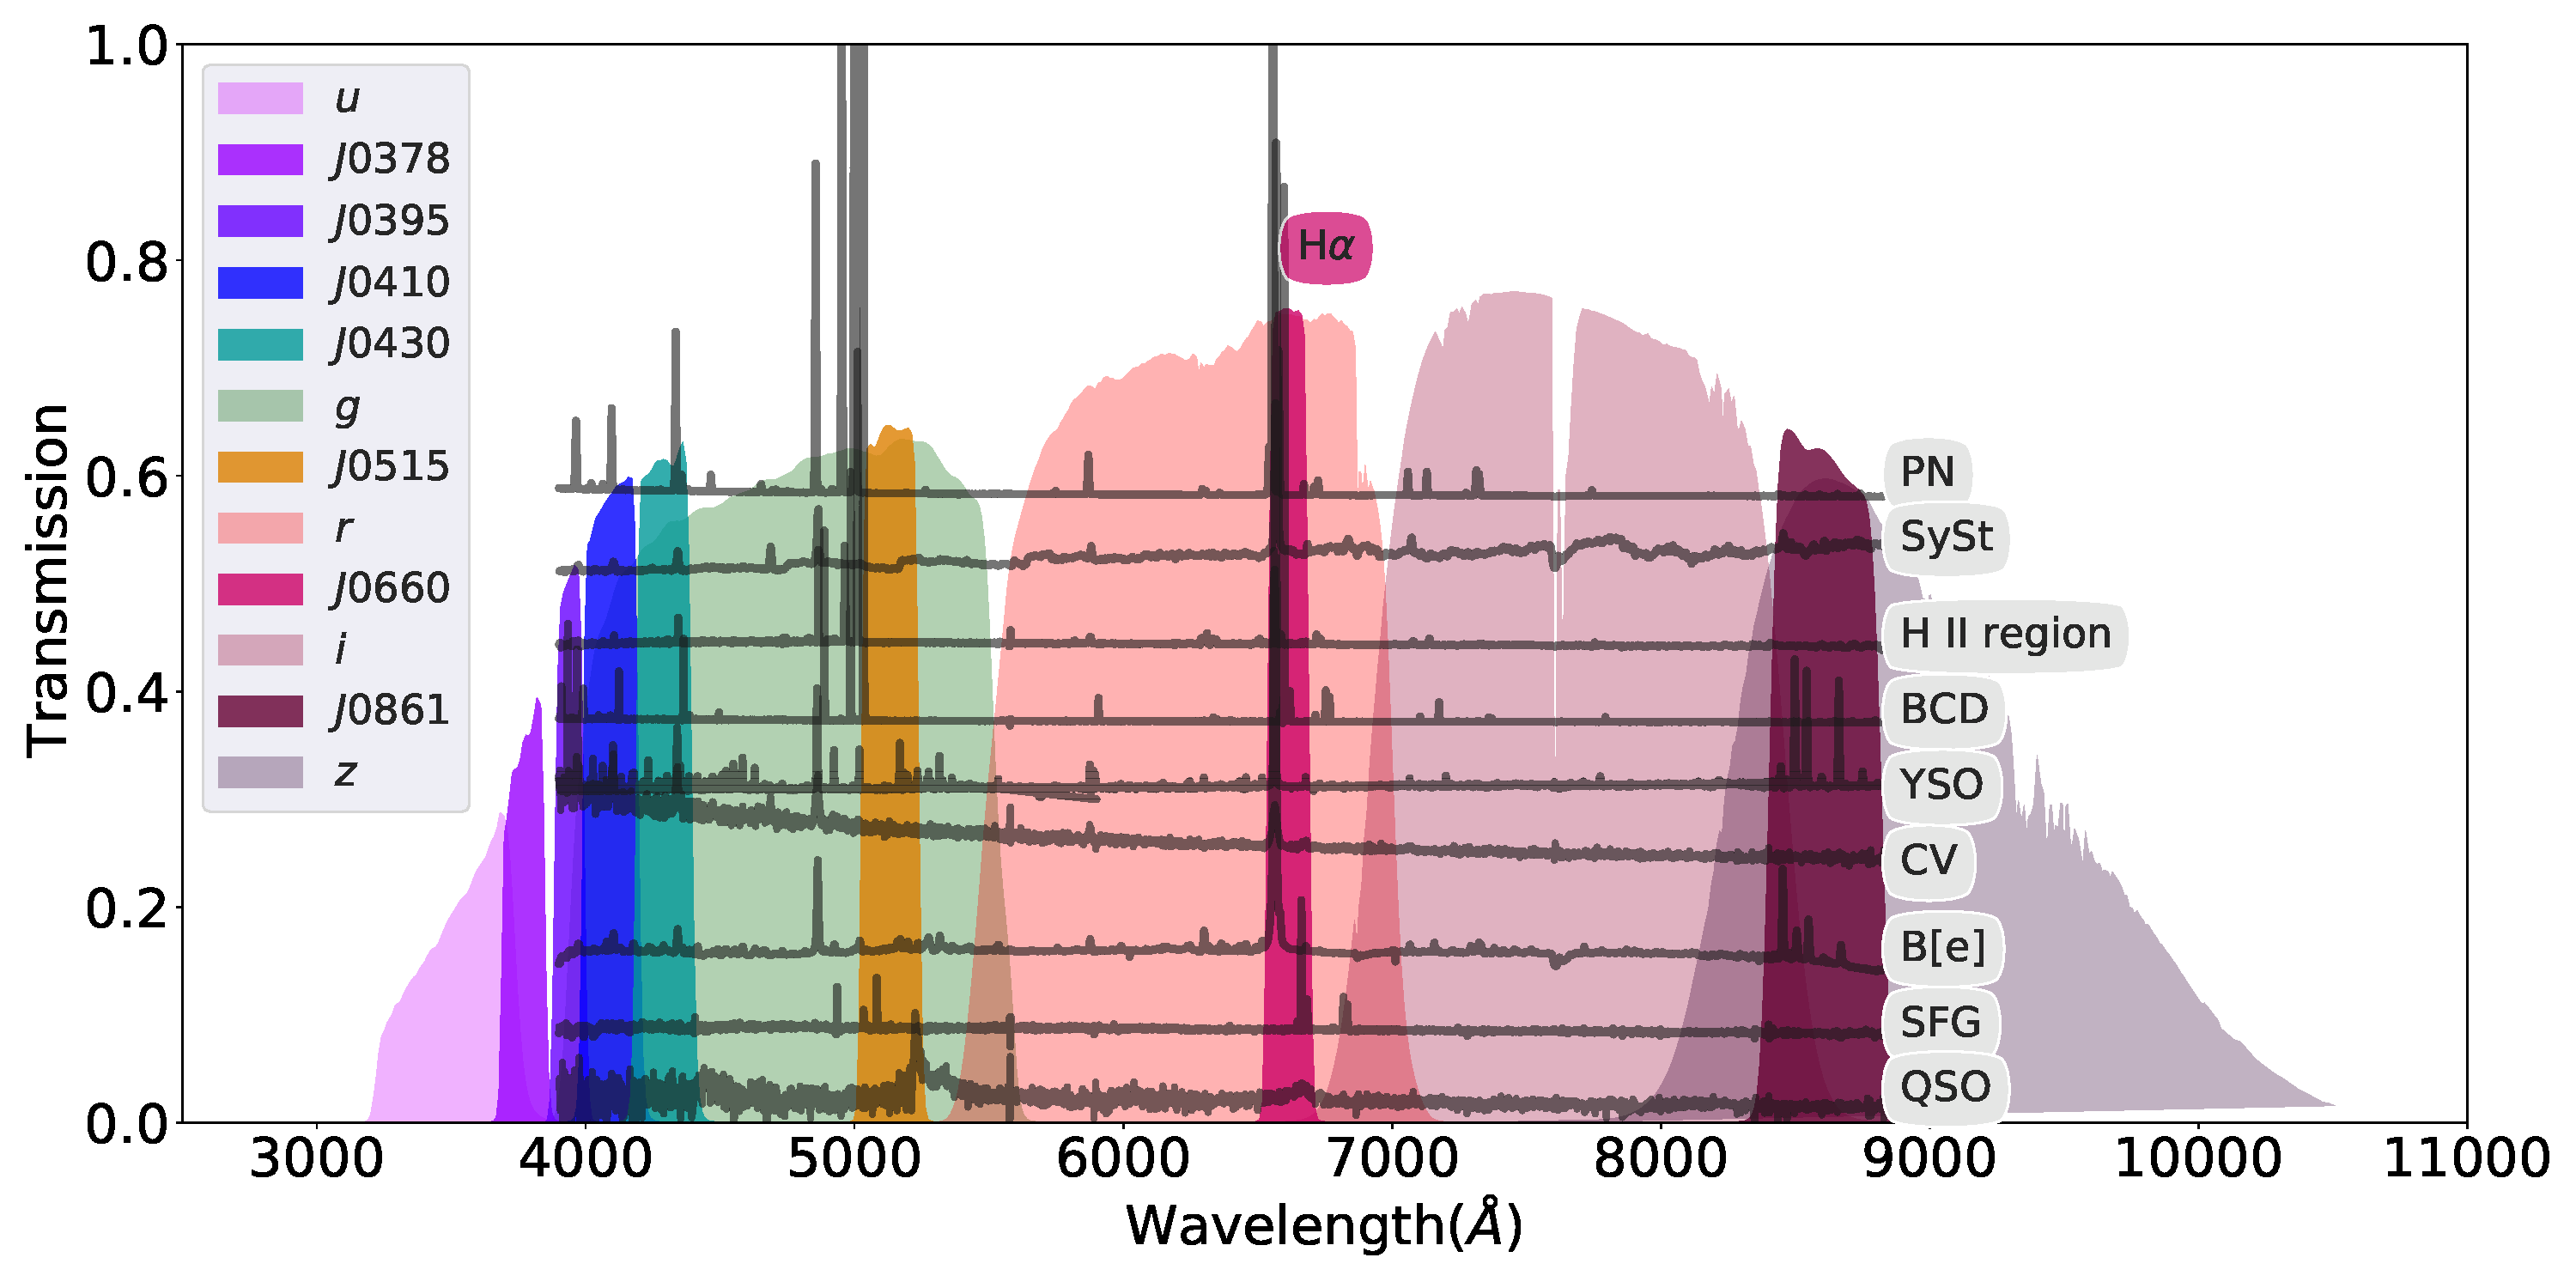
\includegraphics[width=0.9\linewidth]{Figs/splus-filter.pdf}
    \caption{Transmission curves of the S-PLUS filters set. The narrow-band filter $J0660$ detects the H$\alpha$ emission line. Over-plotted are different classes of emission line objects, from upper to down PN, SySt ... }
    \label{fig:curves}
\end{figure}


\section{Methodology}
\label{sec:metho}

We first constructed a sub-sample from all S-PLUS DR3 from which we applied an iterative and automatic technique to select objects with an excess of H{$\alpha$} emission line,  as we describe below:

\subsection{Initial selection sample}
\label{sec:}

The firts step in our selection procedure consist in the following criteria to guarantee the quality of the observations of the objects:

\begin{enumerate}
\item The sources must have detection in the filters: $r$, $i$ and $J$0660. To assure that we select object must have error minor or equal to 0.2 in each of three filter.

\item Must have an $r$ magnitude until $r = 21$.
  
\end{enumerate}

\subsection{Finding the main stellar locus and selecting the H{$\alpha$ emitters} }
\label{sec:}

Once the initial cut were made, we proceed to select the objects with an excess of H{$\alpha$} wich is represent relatively high value of the filter $J$0660 in comparison with r-band filter. For that we first divided our sub-sample in for magnitude bins using the $r$-band magnitudes. The bins have the follow distribution:

\begin{itemize}
\item 1 bin- objects with magnitude in the $r$-band $r < 16$
\item 2 bin- objects with magnitude in the $r$-band $16 \leq r < 18$
\item 3 bin- objects with magnitude in the $r$-band $18 \leq r < 20$
\item 4 bin- objects with magnitude in the $r$-band $20 \leq r < 21$
  
\end{itemize}

To select t sn
\citet{Witham:2008} presented a catalogue of point-sources H{$\alpha$} emission objects identified in IPHAS. 

To select the emission lines we used the same method created and implemented by \citet{Witham:2008} its possible to do that because the S-PLUS has similar filters that the IPHAS project, which are $r$, $J$0660 and $i$. This technique was used by \citet{Scaringi:2013} to identify blue objects with excess of H{$\alpha$} and after that \citet{Wevers:2017} also applied this methodology to create catalogue of candidate H{$\alpha$} emission showing a high effectiveness.    
Applying the selection criteria to selecting H$\alpha$ emitters. We used the same procedure in  \citet{Wevers:2017}. The objects with H$\alpha$ excess meet the condition:


\begin{equation}
  (r - J0660)_{\mathrm{obs}} - (r - J0660)_{\mathrm{fit}} \geq C \times \sqrt{\sigma^2_{\mathrm{s}} - \sigma^2_{\mathrm{phot}}}
\end{equation}
 
 
where $\sigma_s$ is the root mean squared value of the residuals around
the fit and $\sigma_{phot}$ is the error on the observed $(r - J0660)$ colour

Firts see an aproximation of the  4$\sigma$ cut away from the ariginal fit.

\begin{figure*}
  \setlength\tabcolsep{0pt}
  \setkeys{Gin}{width=0.5\linewidth}
  \begin{tabular}{ll}
    (a) & (b) \\
    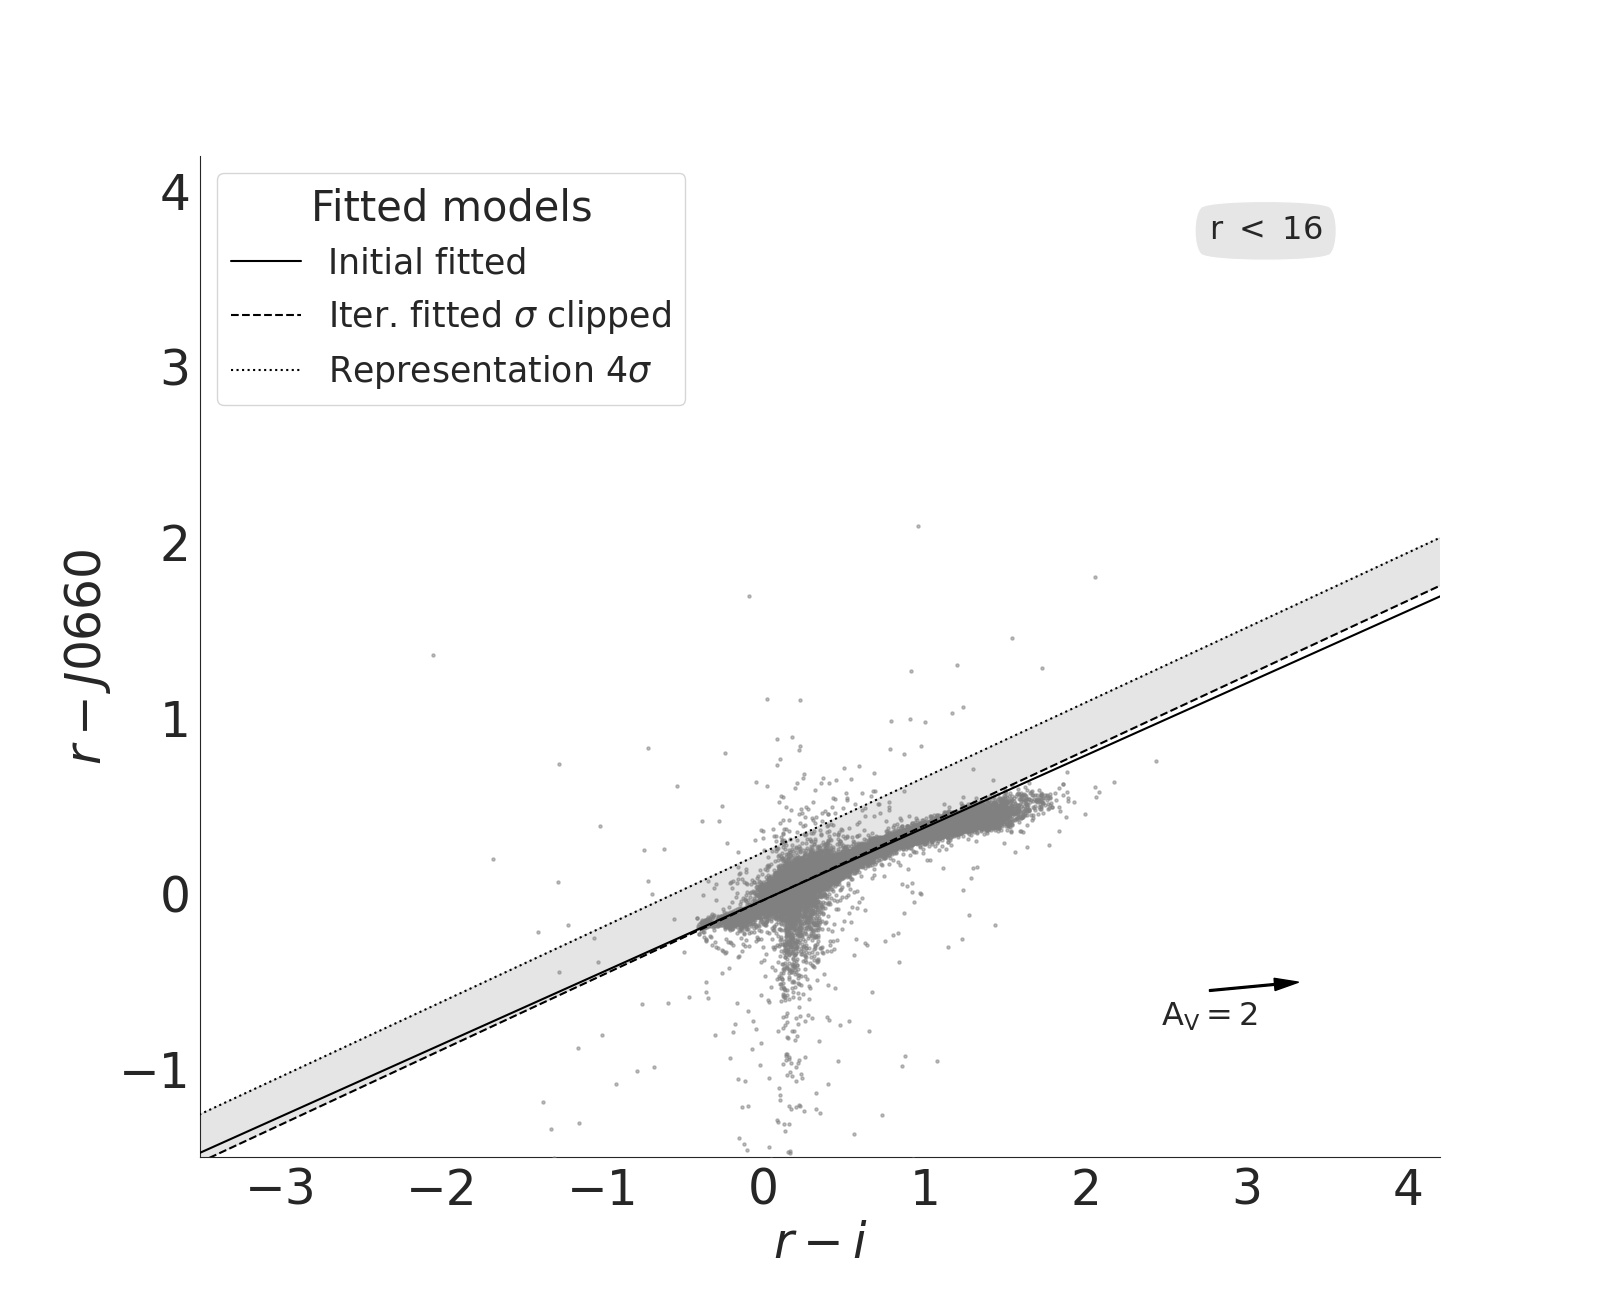
\includegraphics[trim=10 0 65 20, clip]{Figs/diagram-DR3-errorFlag0-3f-16r}
    & 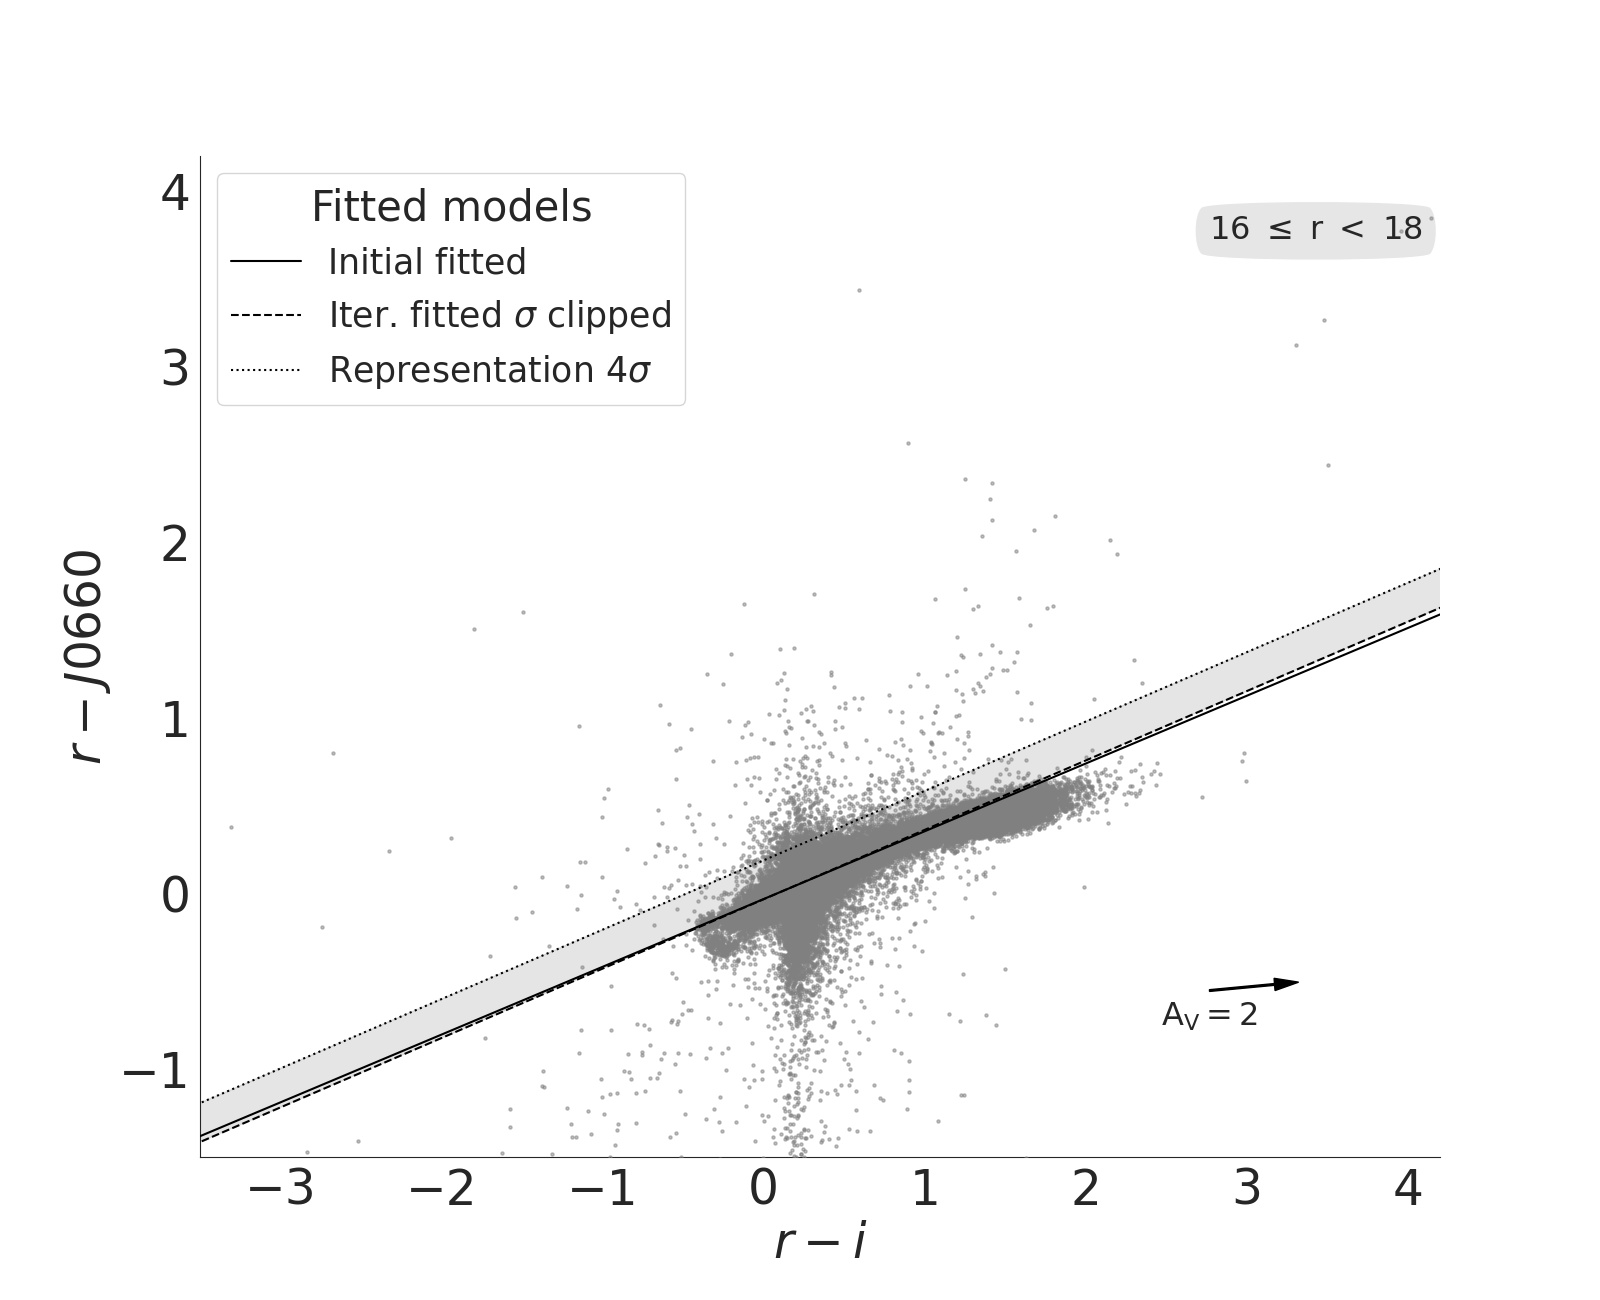
\includegraphics[trim=10 0 65 20, clip]{Figs/diagram-DR3-errorFlag0-3f-16r18}\\
    (c) & (d) \\
    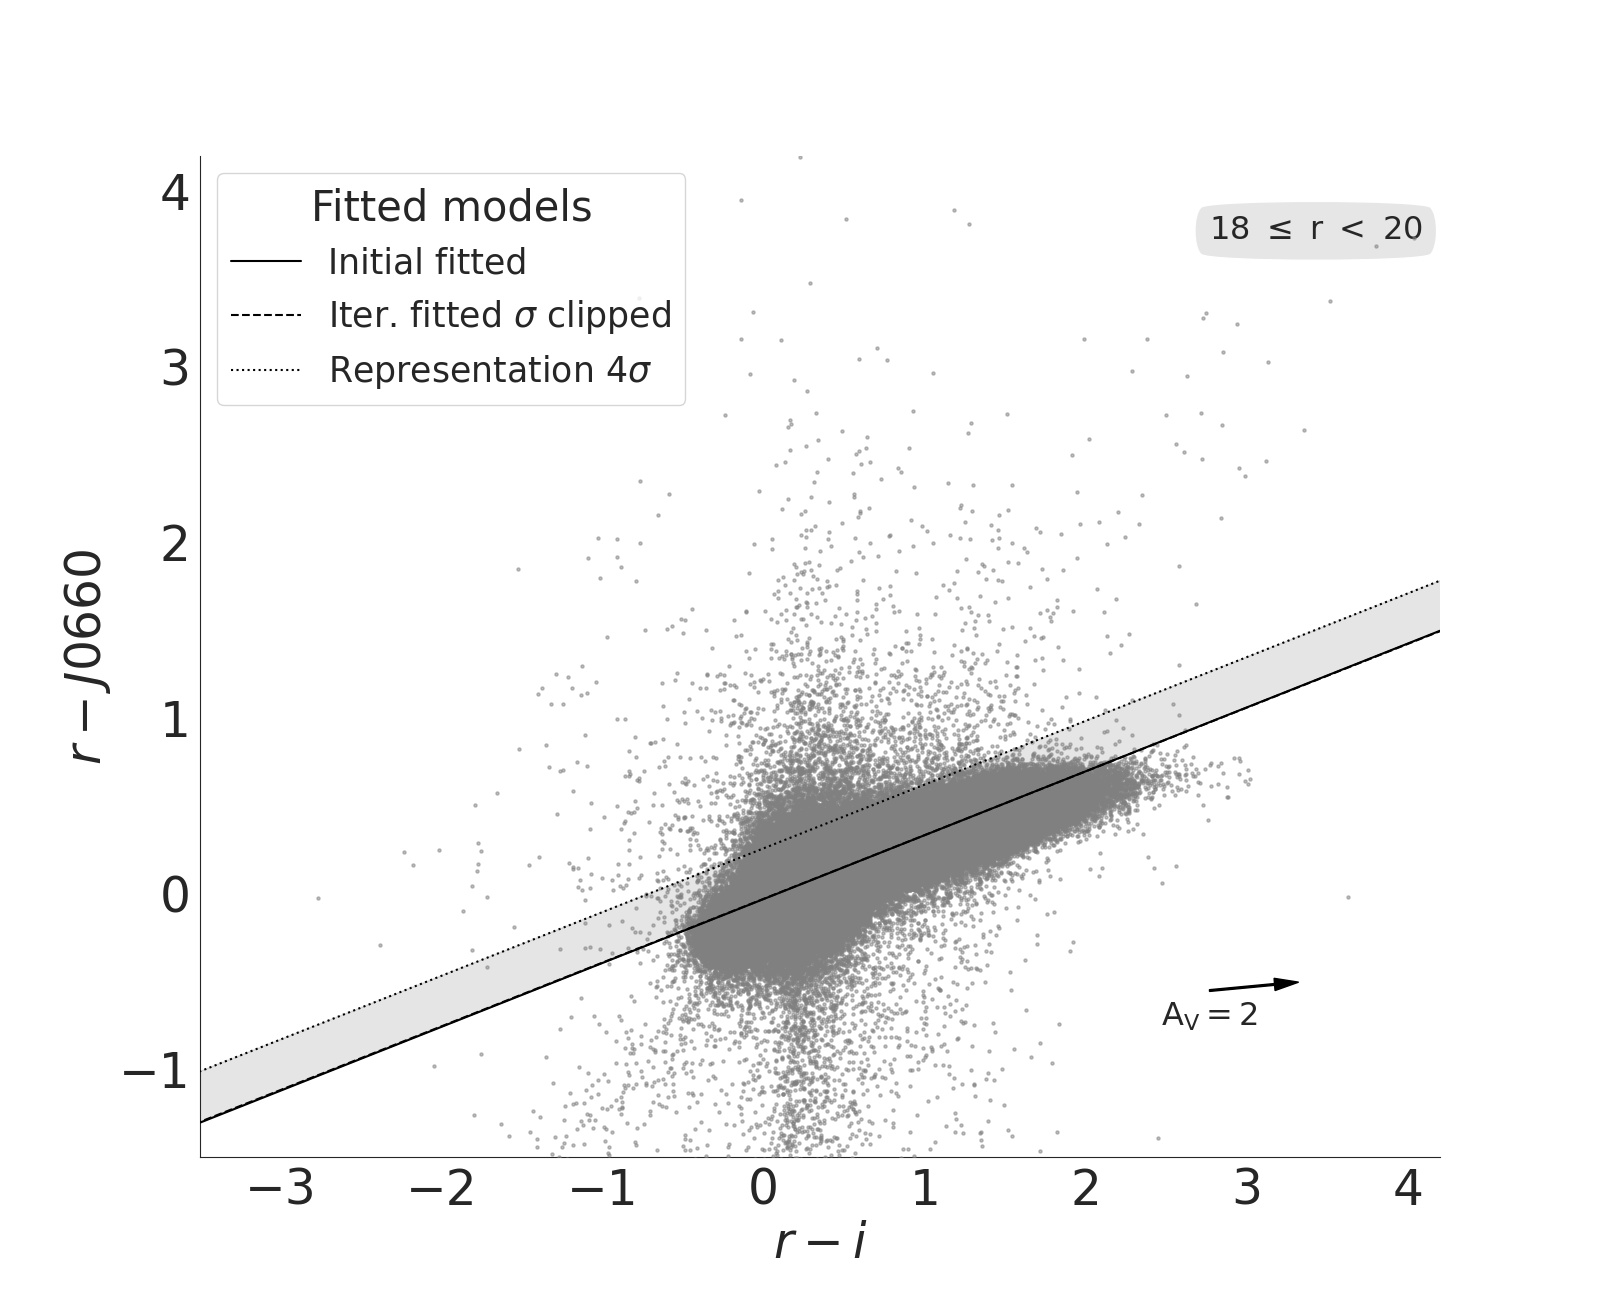
\includegraphics[trim=10 0 65 20, clip]{Figs/diagram-DR3-errorFlag0-3f-18r20}
    & 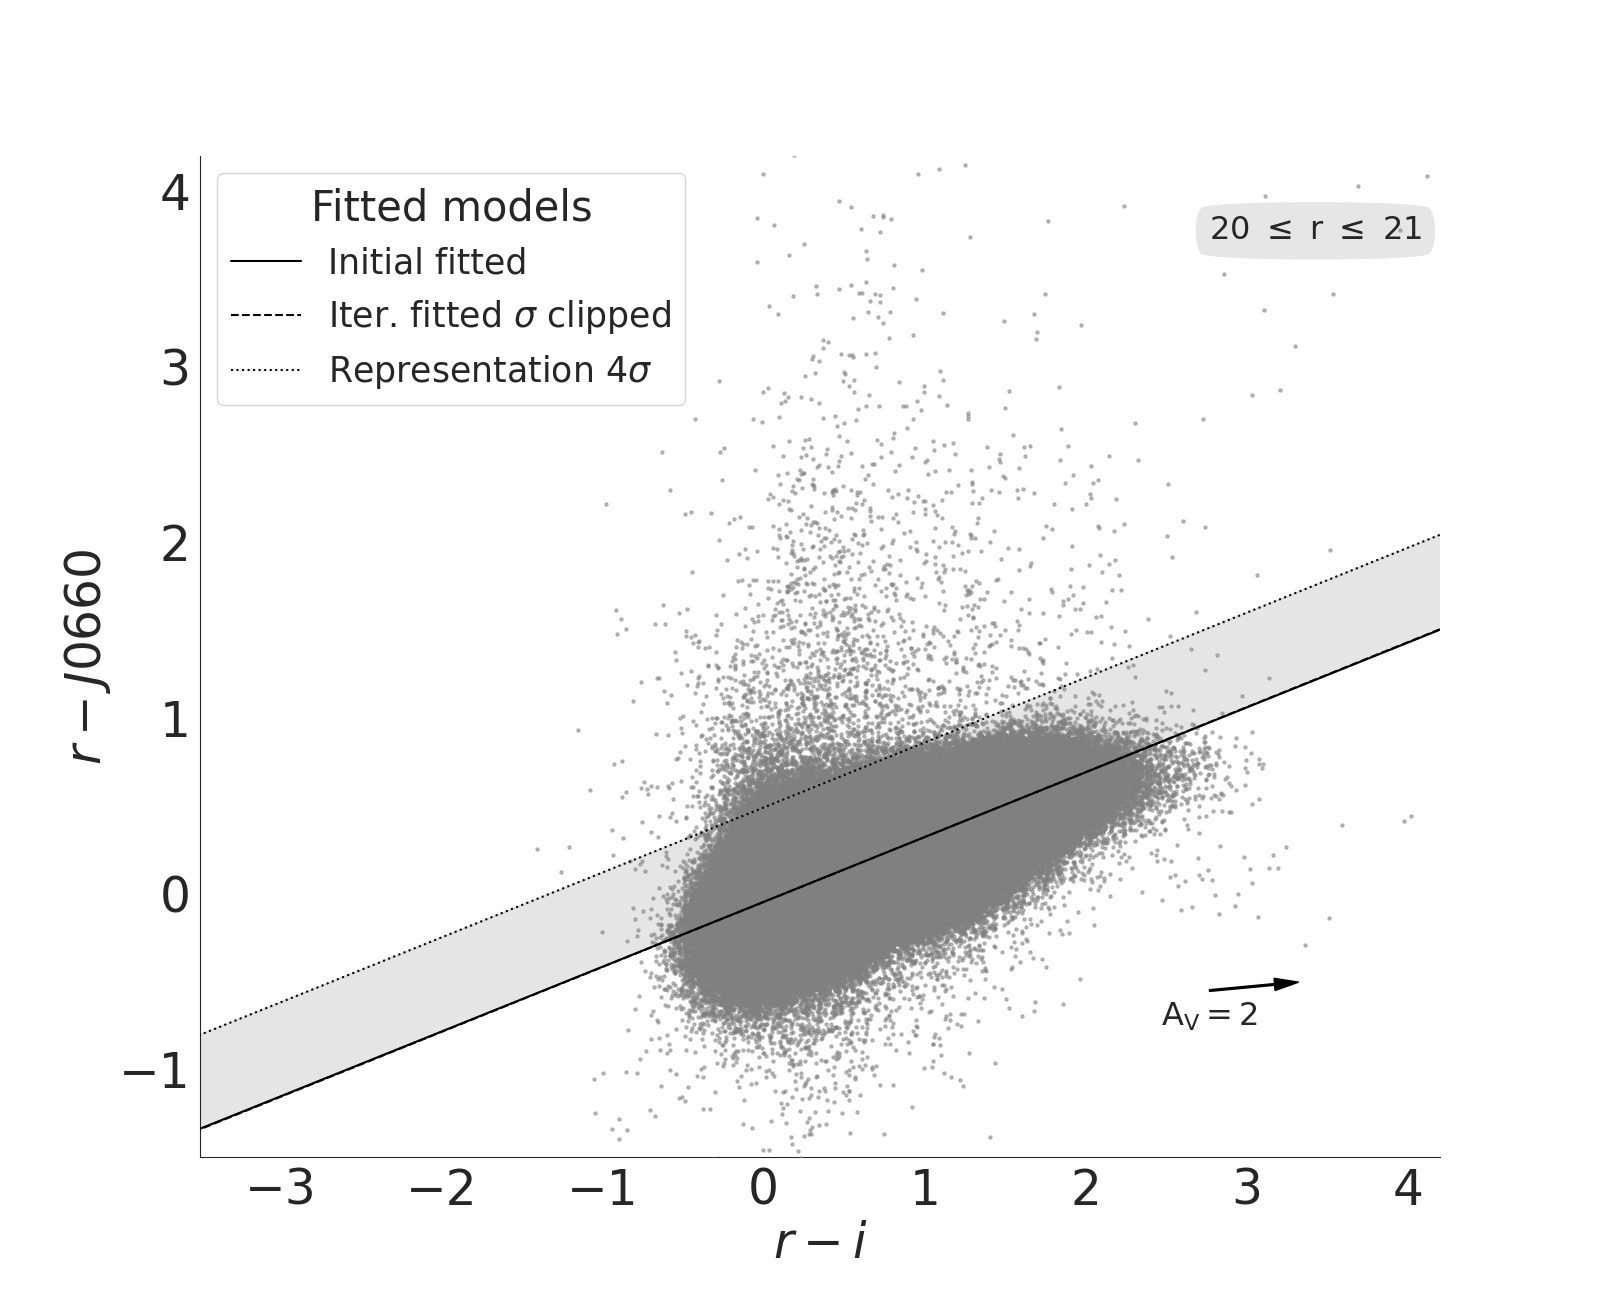
\includegraphics[trim=10 0 65 20, clip]{Figs/diagram-DR3-errorFlag0-3f-20r21}\\
  \end{tabular}
  \caption{An illustration of the selection criteria used to identify strong emission-line objects via colour-colour plots. The data shown here are all from the
S-PLUS DR3. The data are split up into four magnitude bins, as shown in the four panels. Objects with H{$\alpha$} excess should be located near the top of the colour-colour plots. The thin red lines illustrate the original least-squares fit to all the data (grey points). The thin blue lines represent the final fits to the upper locus of points obtained by applying an iterative
σ -clipping technique to the initial fit. The actual cuts used to select H{$\alpha$} emitters are shown by the thick dashed lines. If the cut was based on the initial (final)
fit, it is shown in red (blue). Objects selected as Hα emitters must be located above the cut and are shown as large triangles. Note that the cut lines shown here
are only approximate, as the actual selection criterion also considers the errors on each individual data point. This explains, for example, why an object in the bottom right-hand panel is not selected despite clearly lying above the cut line.}
  \label{fig:criteria-color-plot}
\end{figure*}

In Figure~\ref{fig:criteria-color-plot} is illustrate the selection process.  The black line represent the fit  

\subsection{Maths}
\label{sec:maths} % used for referring to this section from elsewhere


\begin{equation}

    x=\frac{-b\pm\sqrt{b^2-4ac}}{2a}.
	\label{eq:quadratic}
\end{equation}


\subsection{Figures and tables}

\section{Results}
\label{sec:results}

\begin{figure*}
	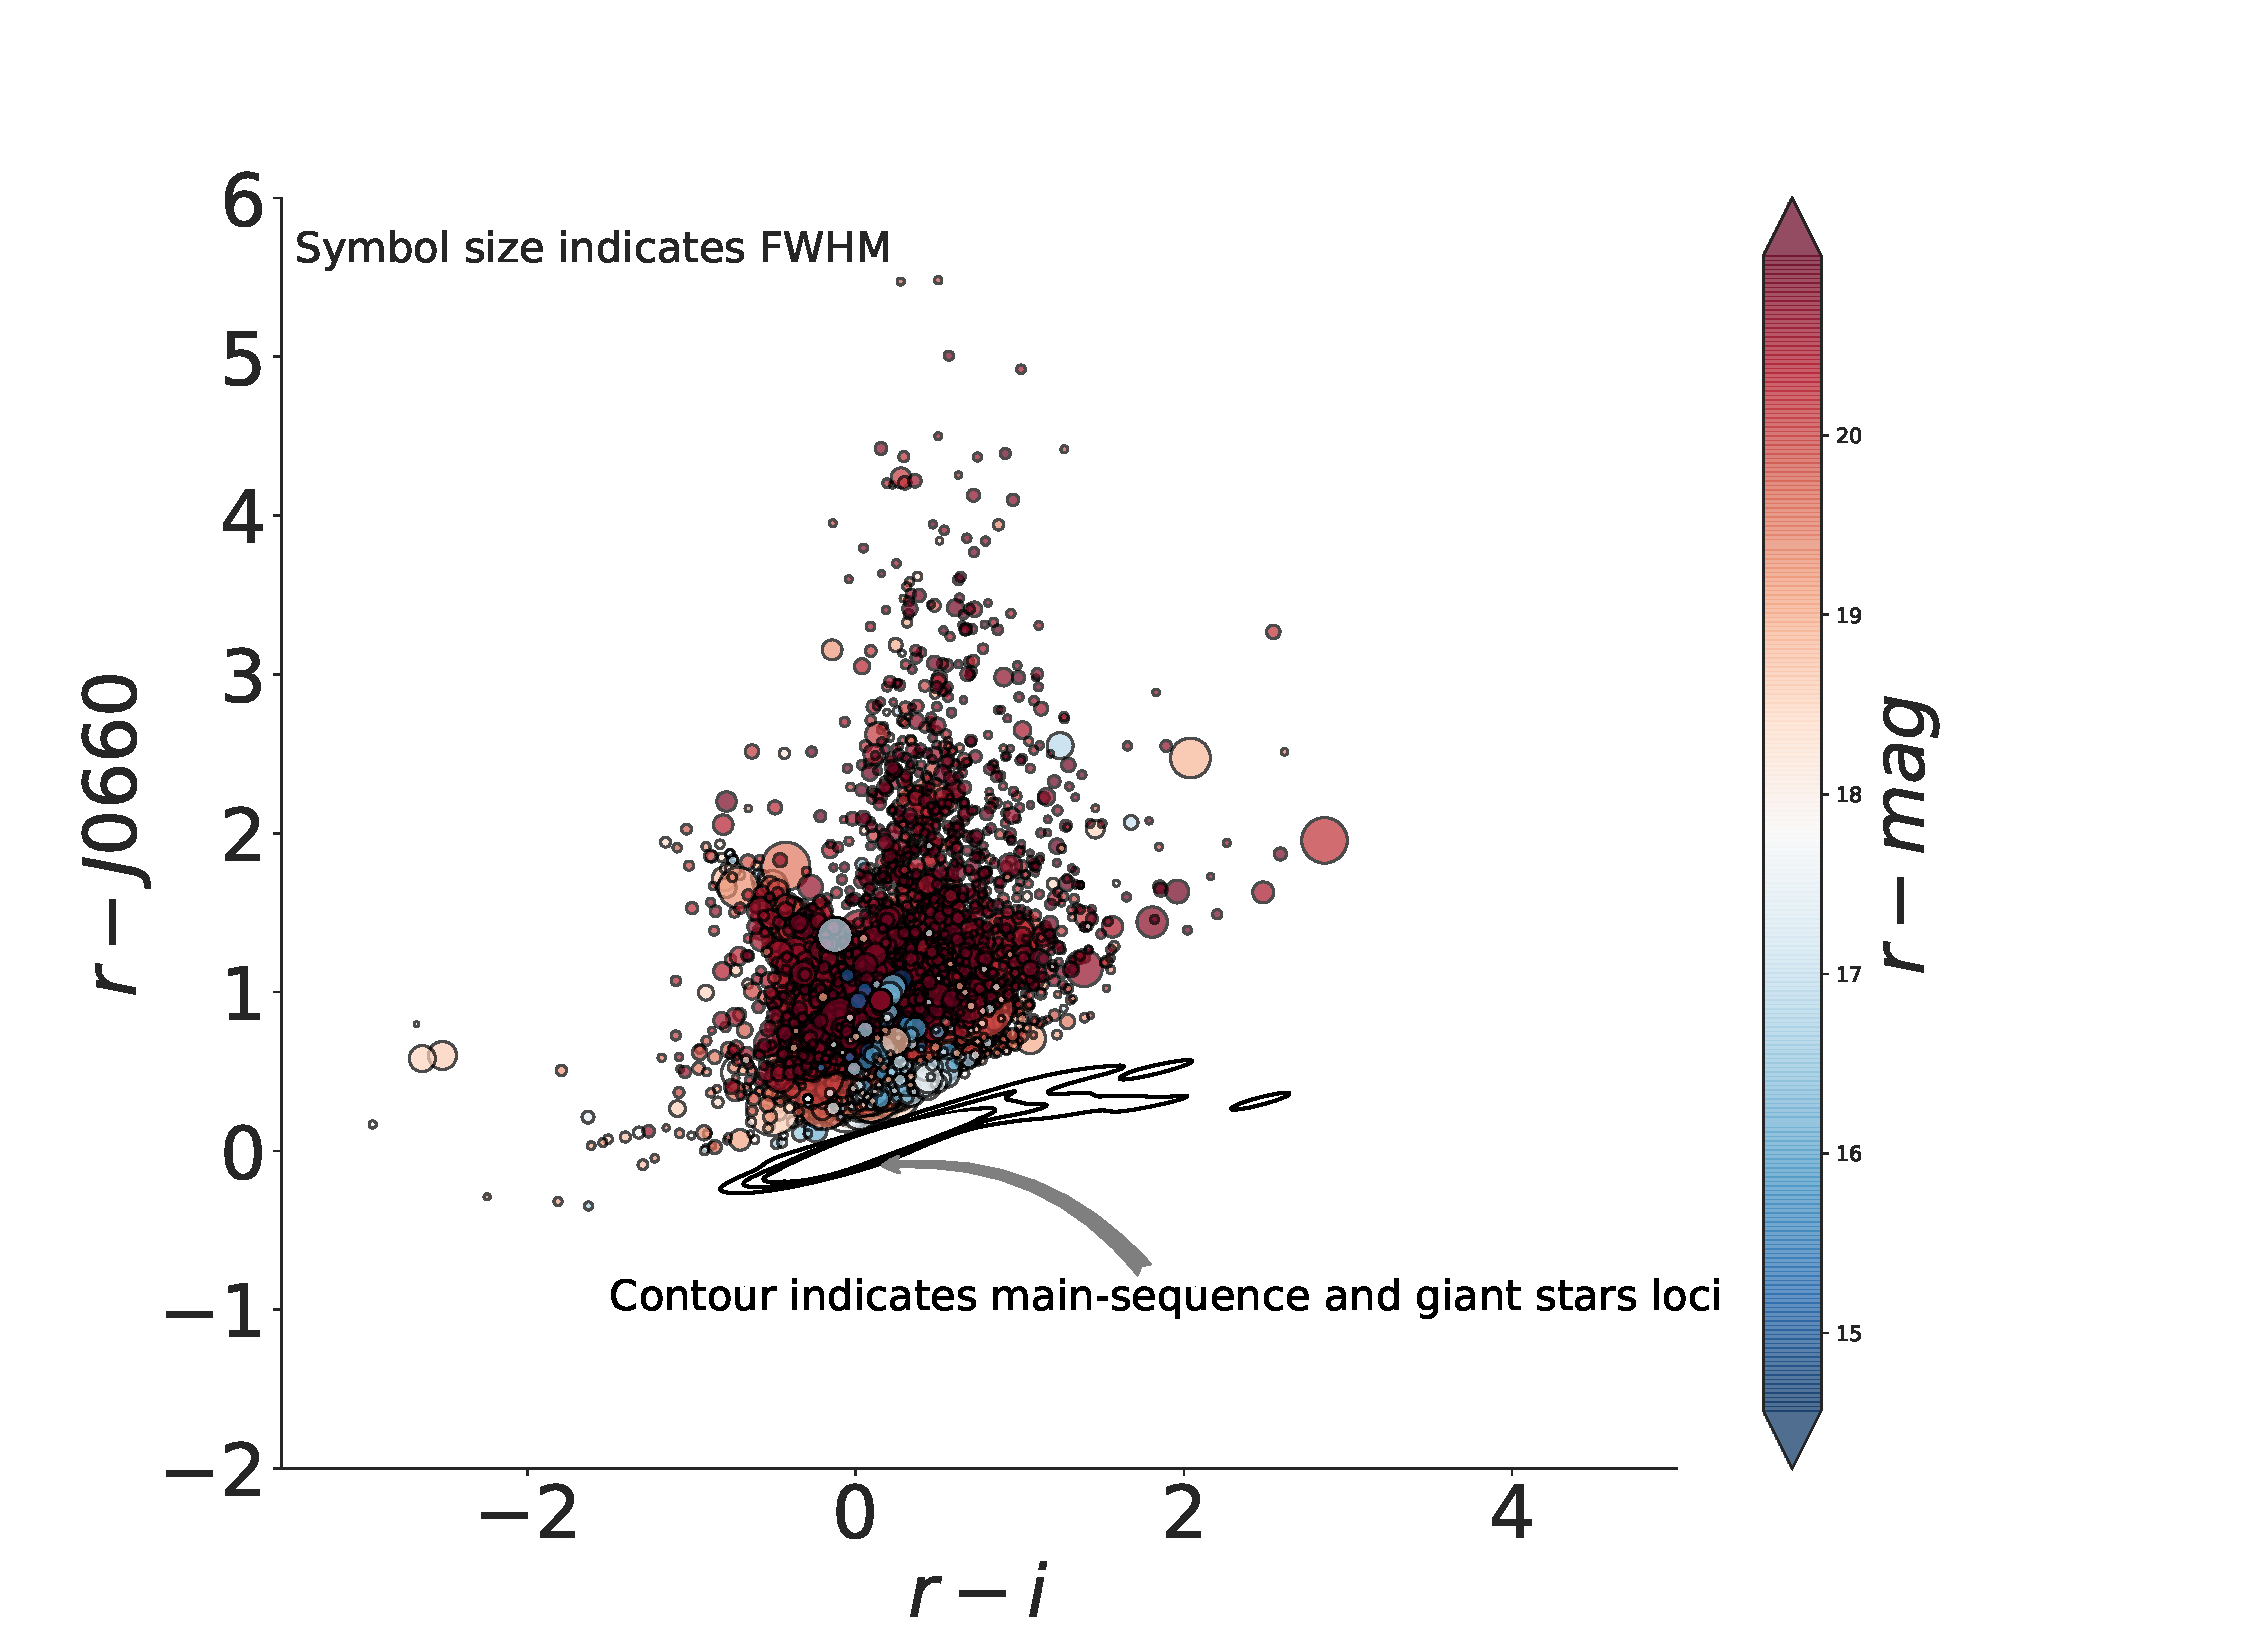
\includegraphics[width=0.9\linewidth]{Figs/final-emitters.pdf}
    \caption{Colour-colour diagram with all the emission line objects selected from S-PLUS DR3. Size of the symbols represent the measured FWHM assuming a Gaussian core (for more detail see \citealt{Fernandes:2021}). Colored bar is the magnitude values in the r-band. The contours represent the synthetic main-sequence and giant stars loci from the library of stellar spectral energy distributions of \citet{Pickles:1998}.}
    \label{fig:emission}
\end{figure*}

\begin{figure*}
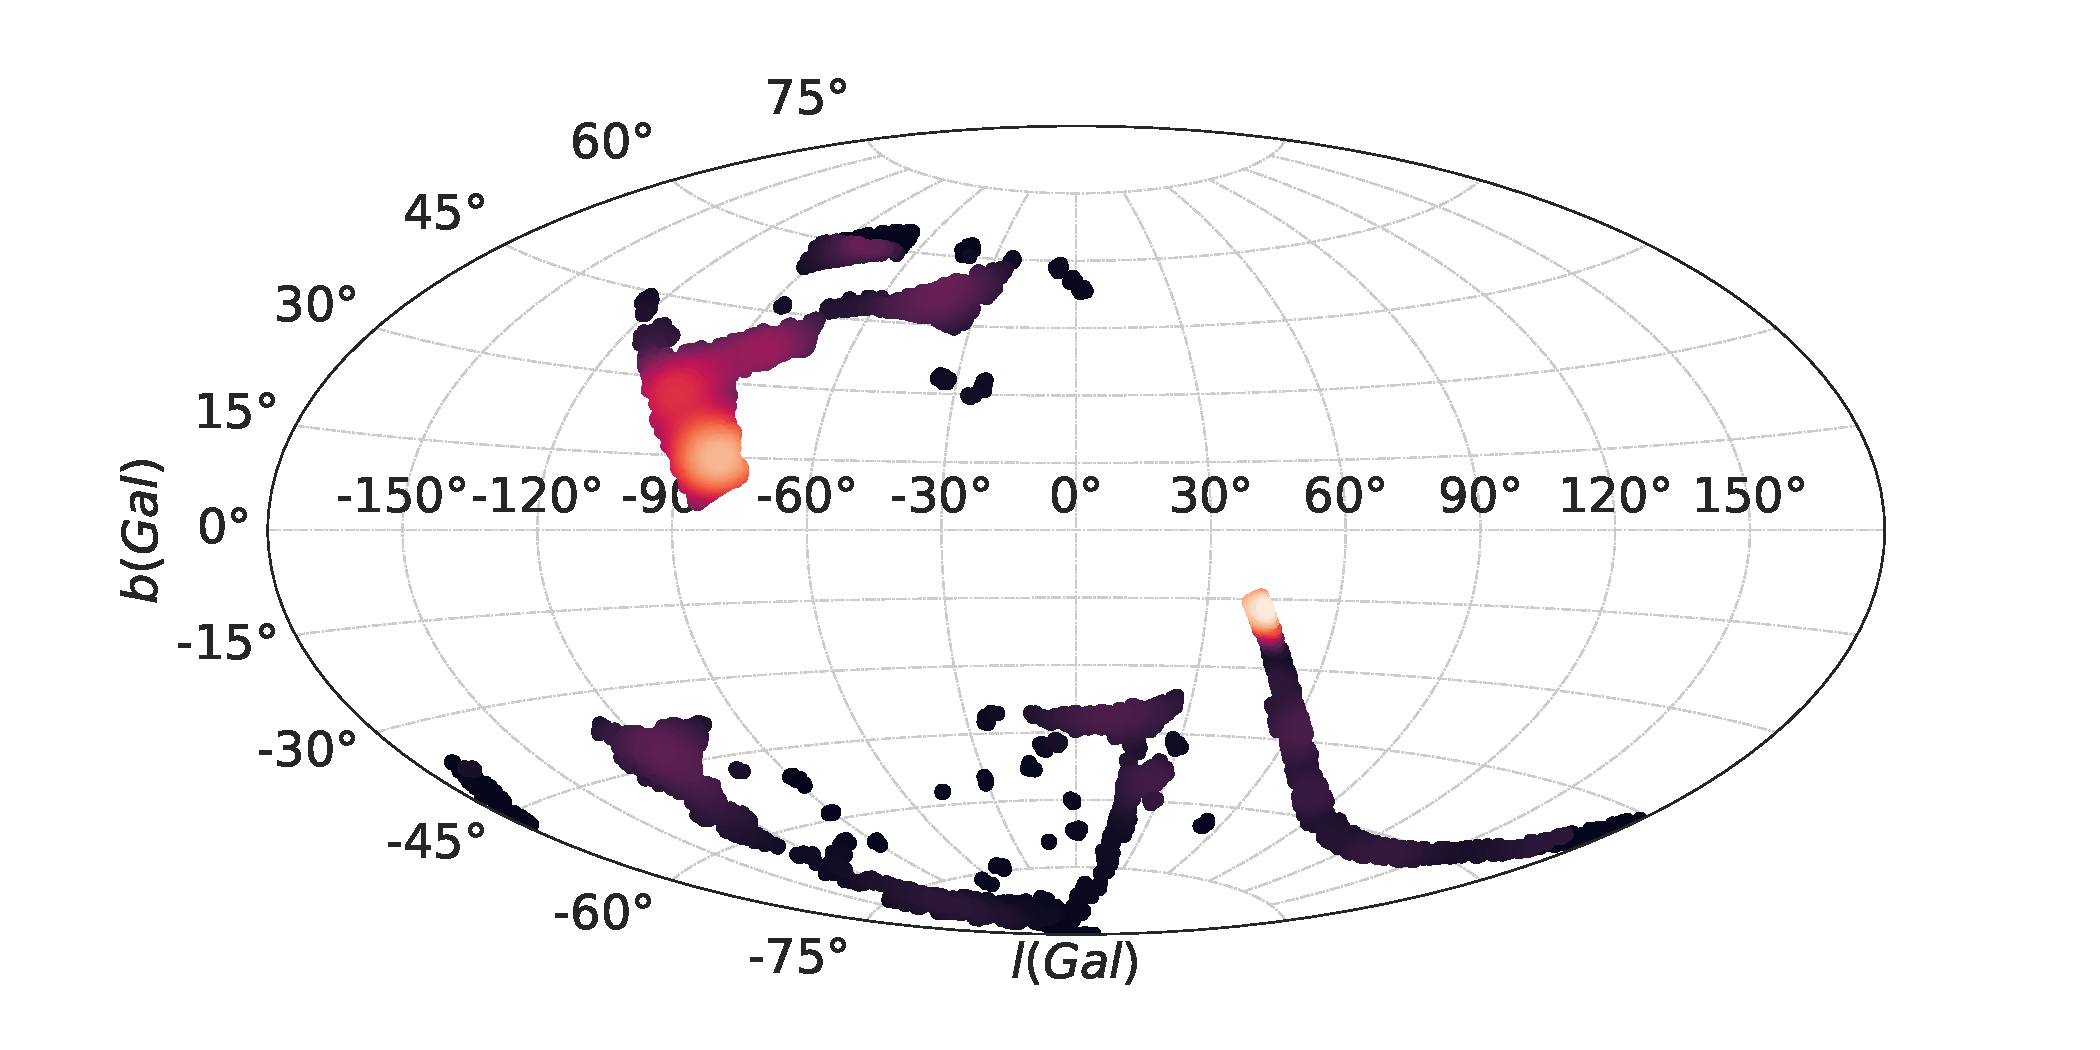
\includegraphics[width=0.9\linewidth]{Figs/halpha-emitters-galactic-aitoff.pdf}
\centering
\llap{\shortstack{%
        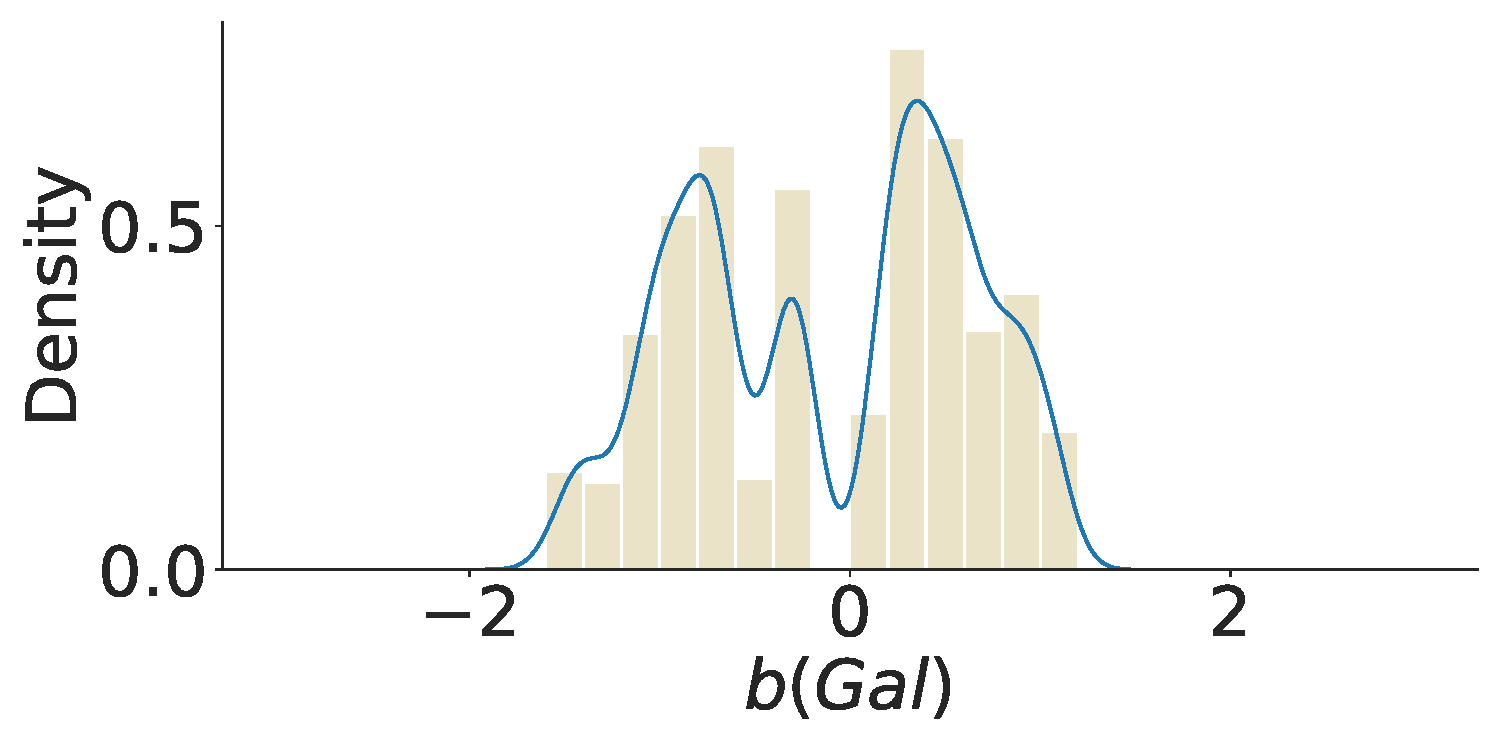
\includegraphics[width=0.25\linewidth, trim=10 10 -40 0]{Figs/distribution-bgalactic.pdf}\\
        \rule{0ex}{1.8in}%
      }
  \rule{1.0in}{0ex}}
\caption{This is my embedded figure}
\end{figure*}


\begin{figure*}
  \begin{tabular}{l l l}
  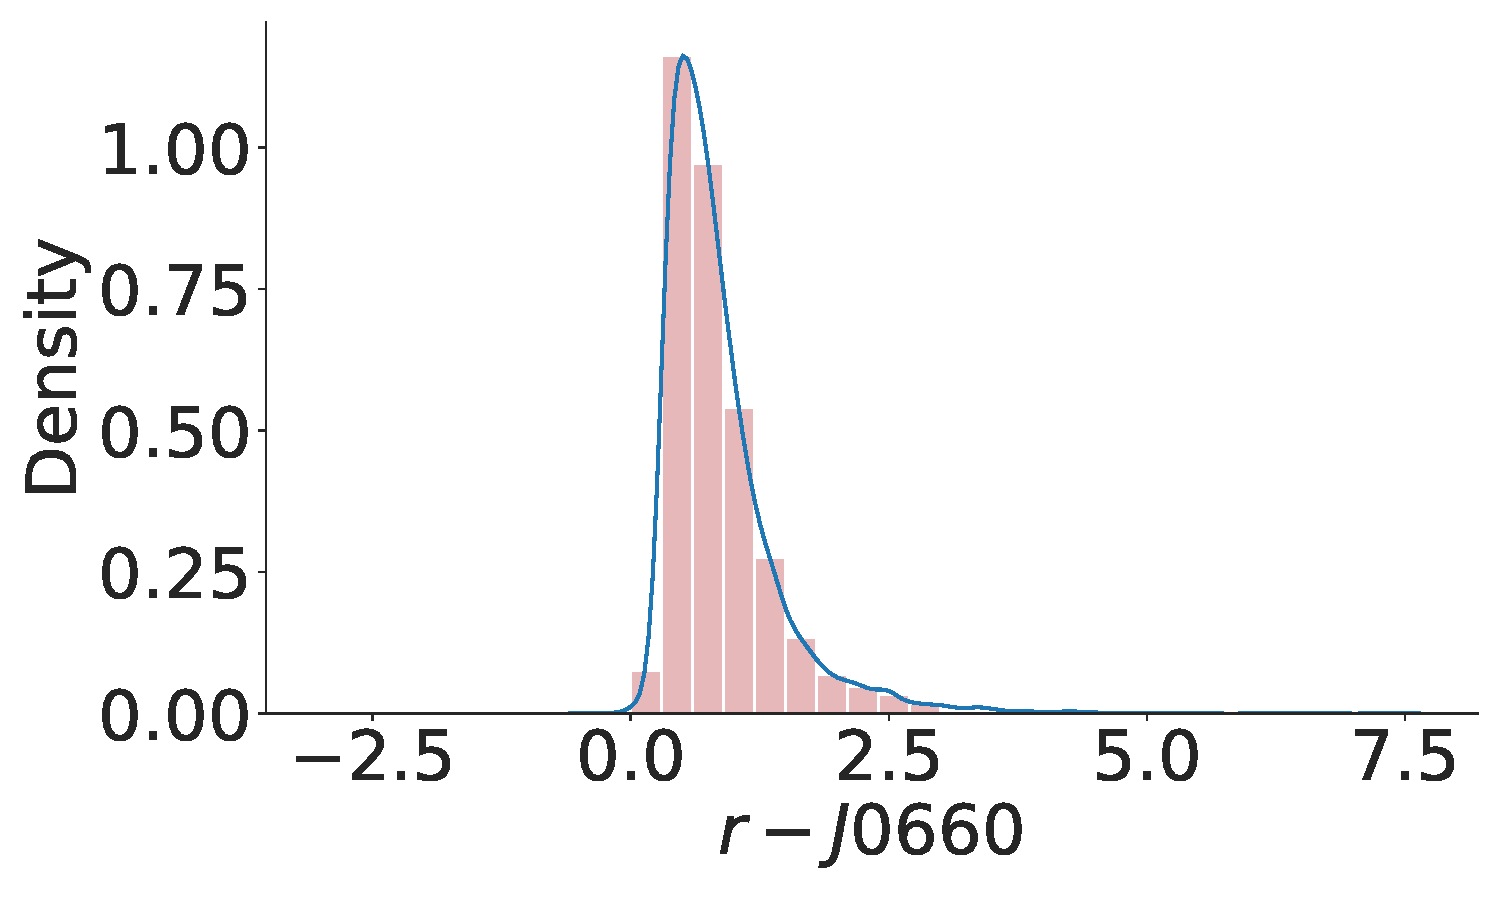
\includegraphics[width=0.7\columnwidth]{Figs/distribution-Halpha.pdf} 
    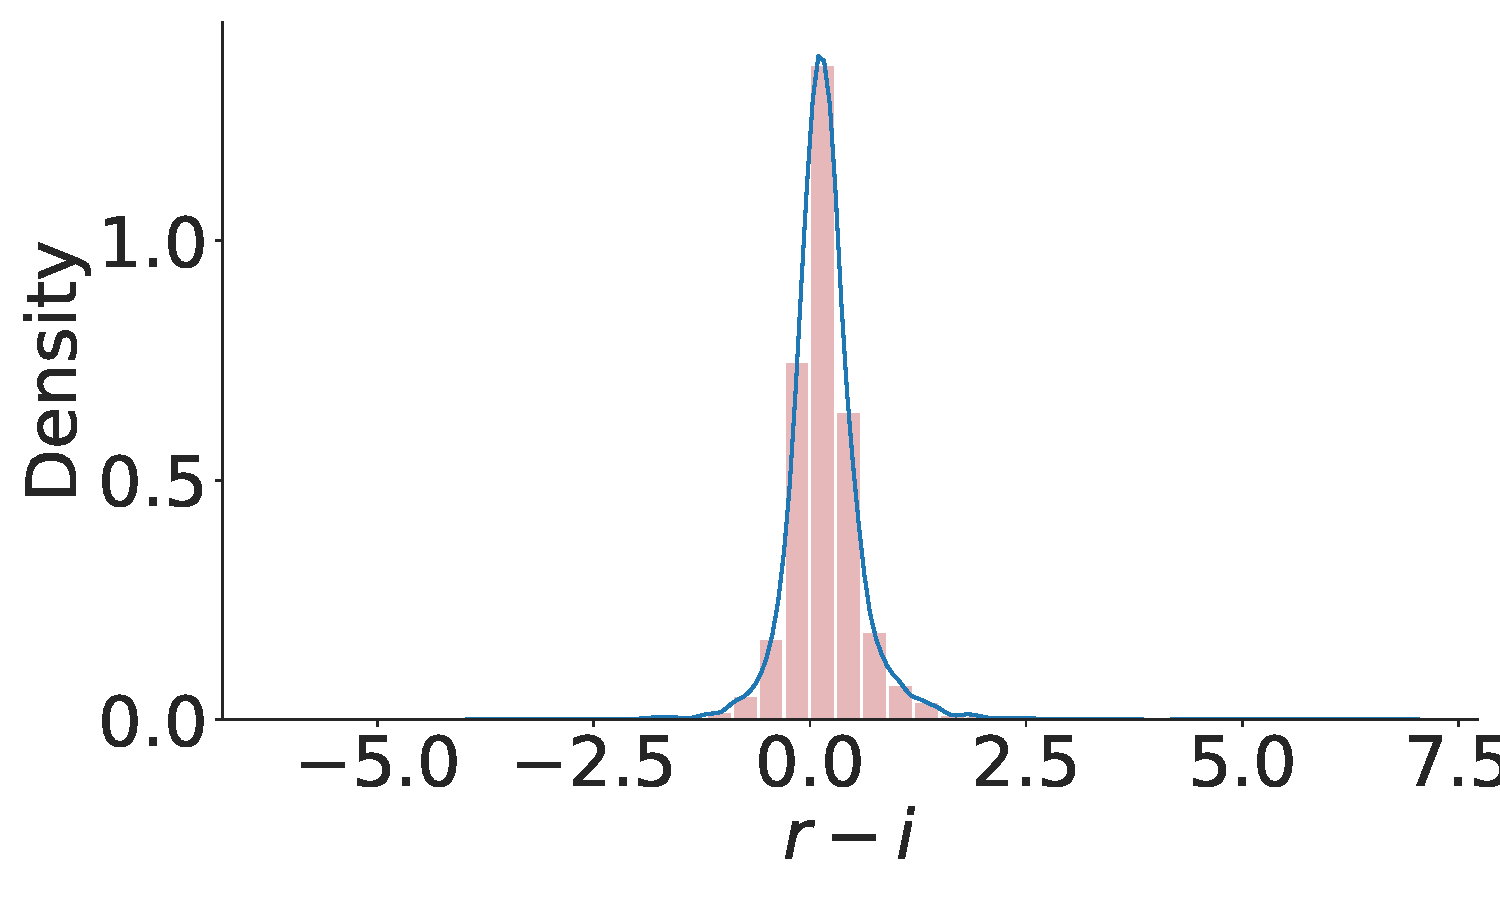
\includegraphics[width=0.7\columnwidth]{Figs/distribution-ri.pdf}
    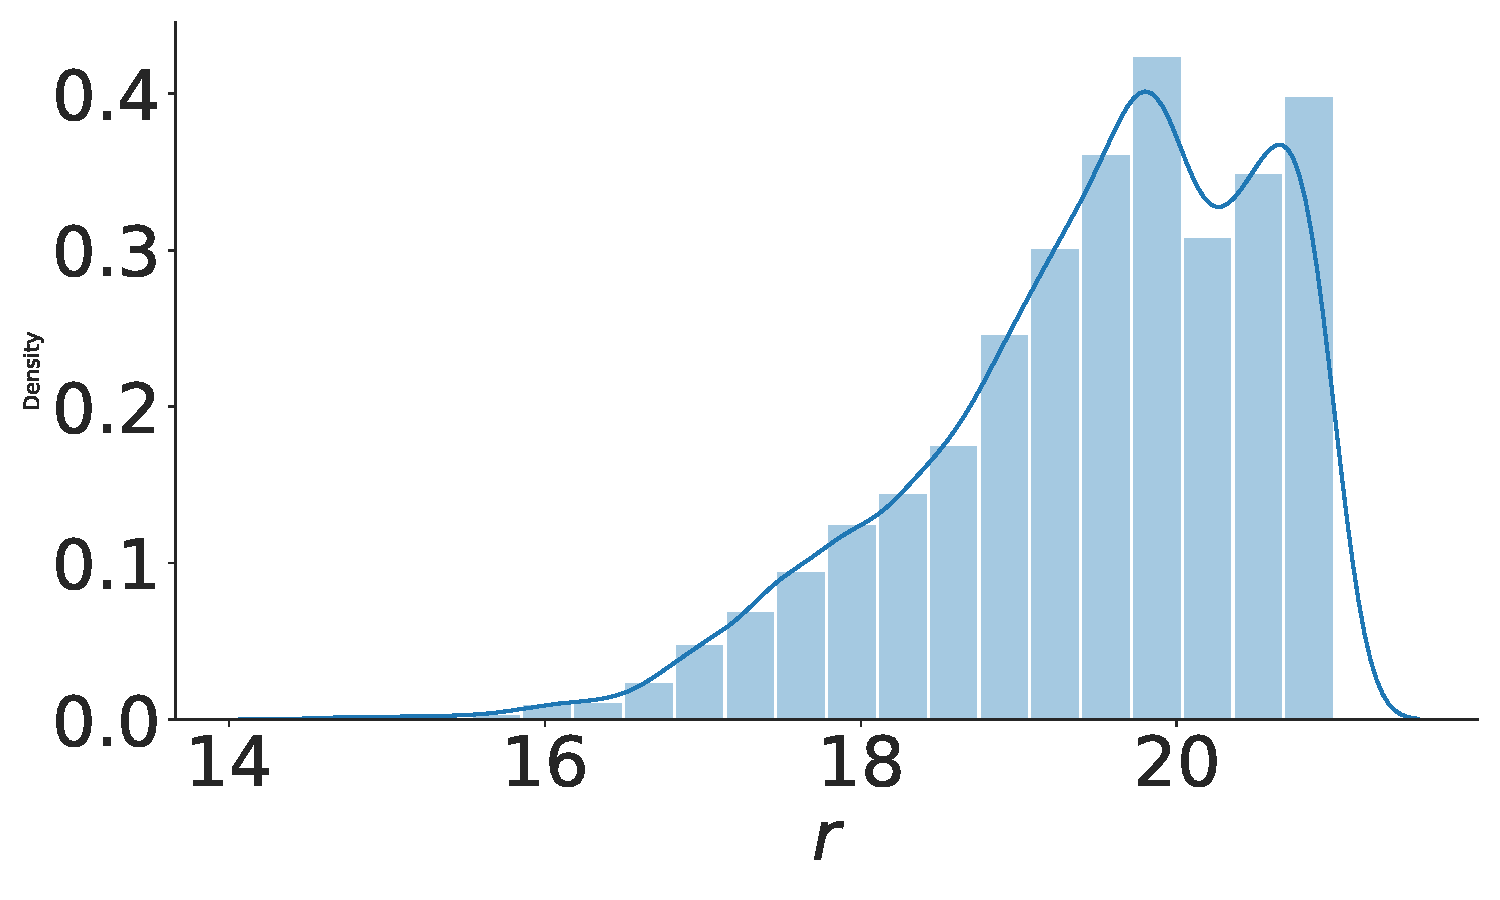
\includegraphics[width=0.7\columnwidth]{Figs/distribution_r.pdf}
  \end{tabular}
    \caption{Emission lines selected...}
    \label{fig:diagram-distri}
\end{figure*}

\begin{figure}
	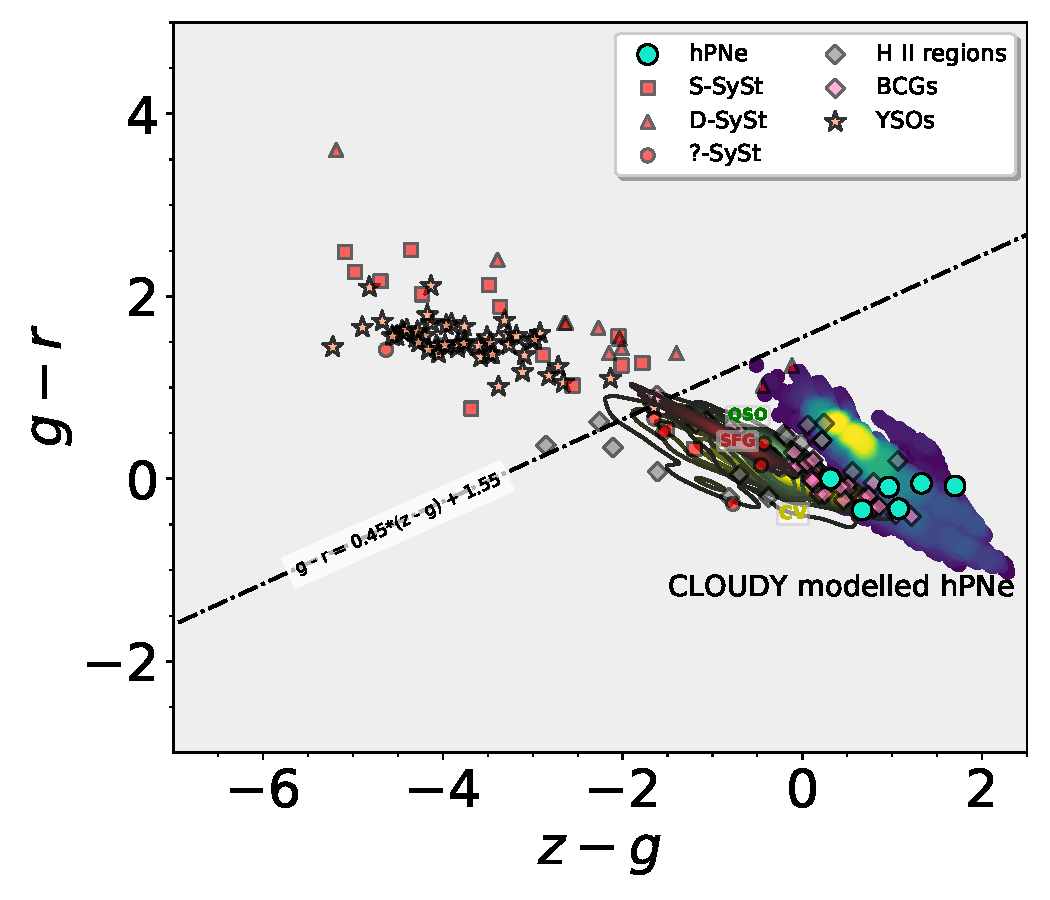
\includegraphics[width=0.9\linewidth]{Figs/Fig-SPLUS-gr-zg.pdf}
    \caption{Classifying...}
    \label{fig:synthetic}
\end{figure}

\begin{figure}
	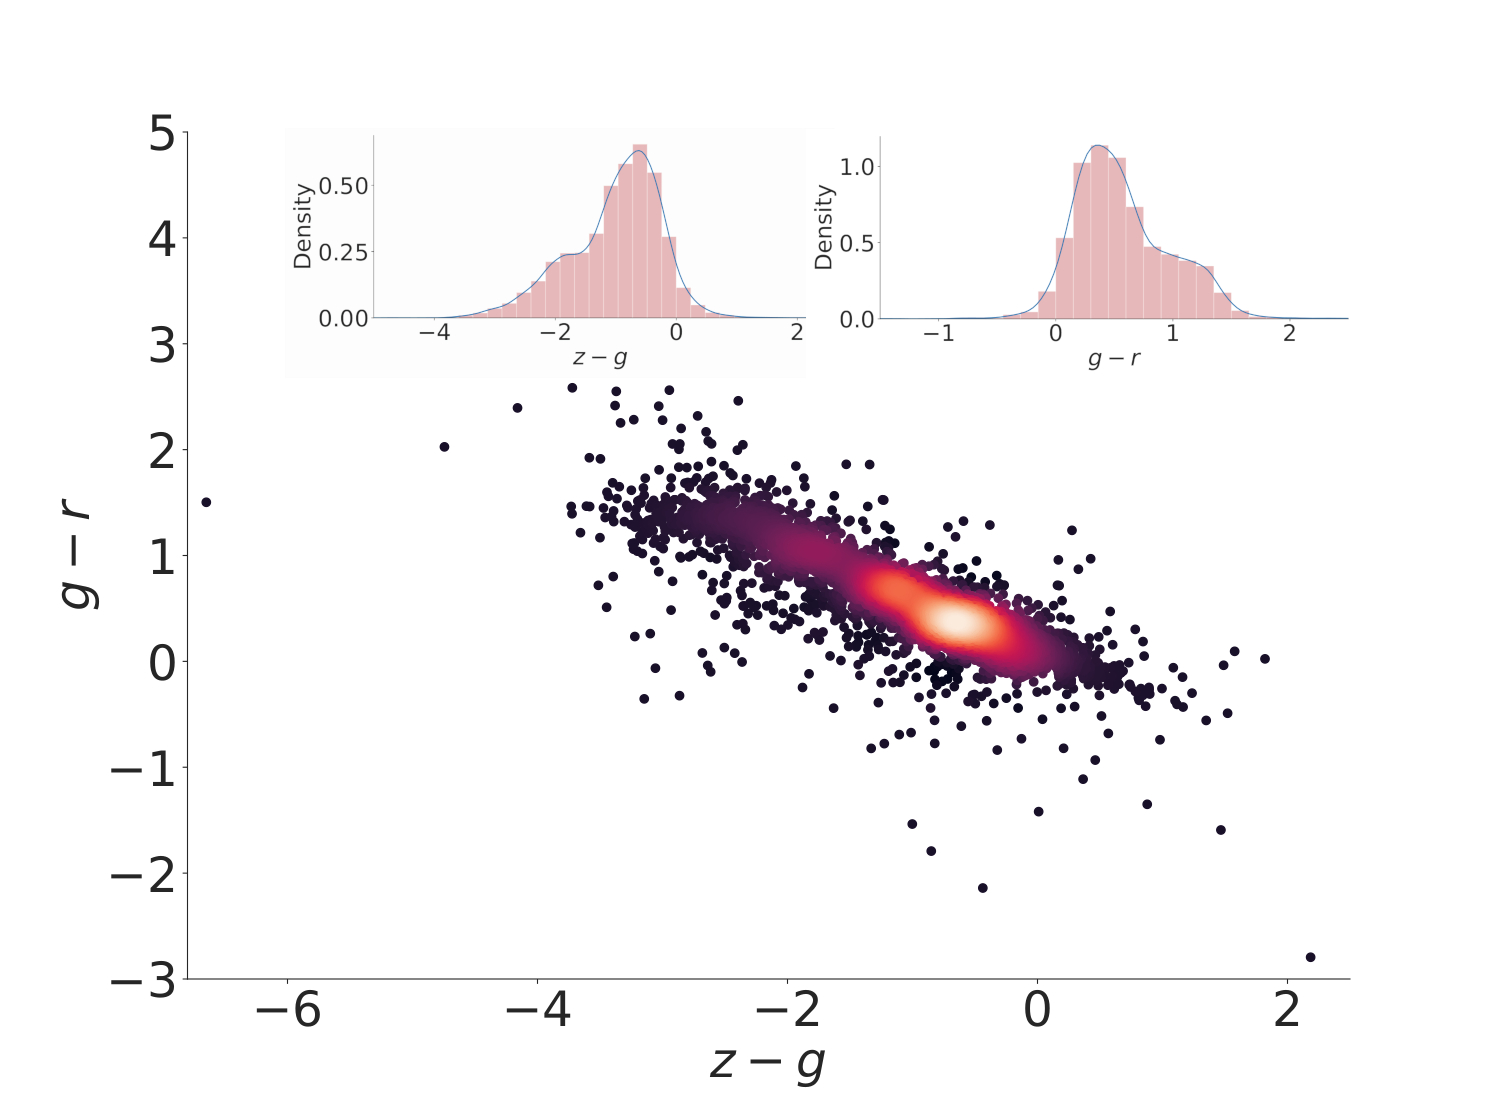
\includegraphics[width=0.9\linewidth]{Figs/red-blue-colorObjects-gr-edit.jpg}
    \caption{Classifying...}
    \label{fig:new-color}
\end{figure}


\begin{figure}
	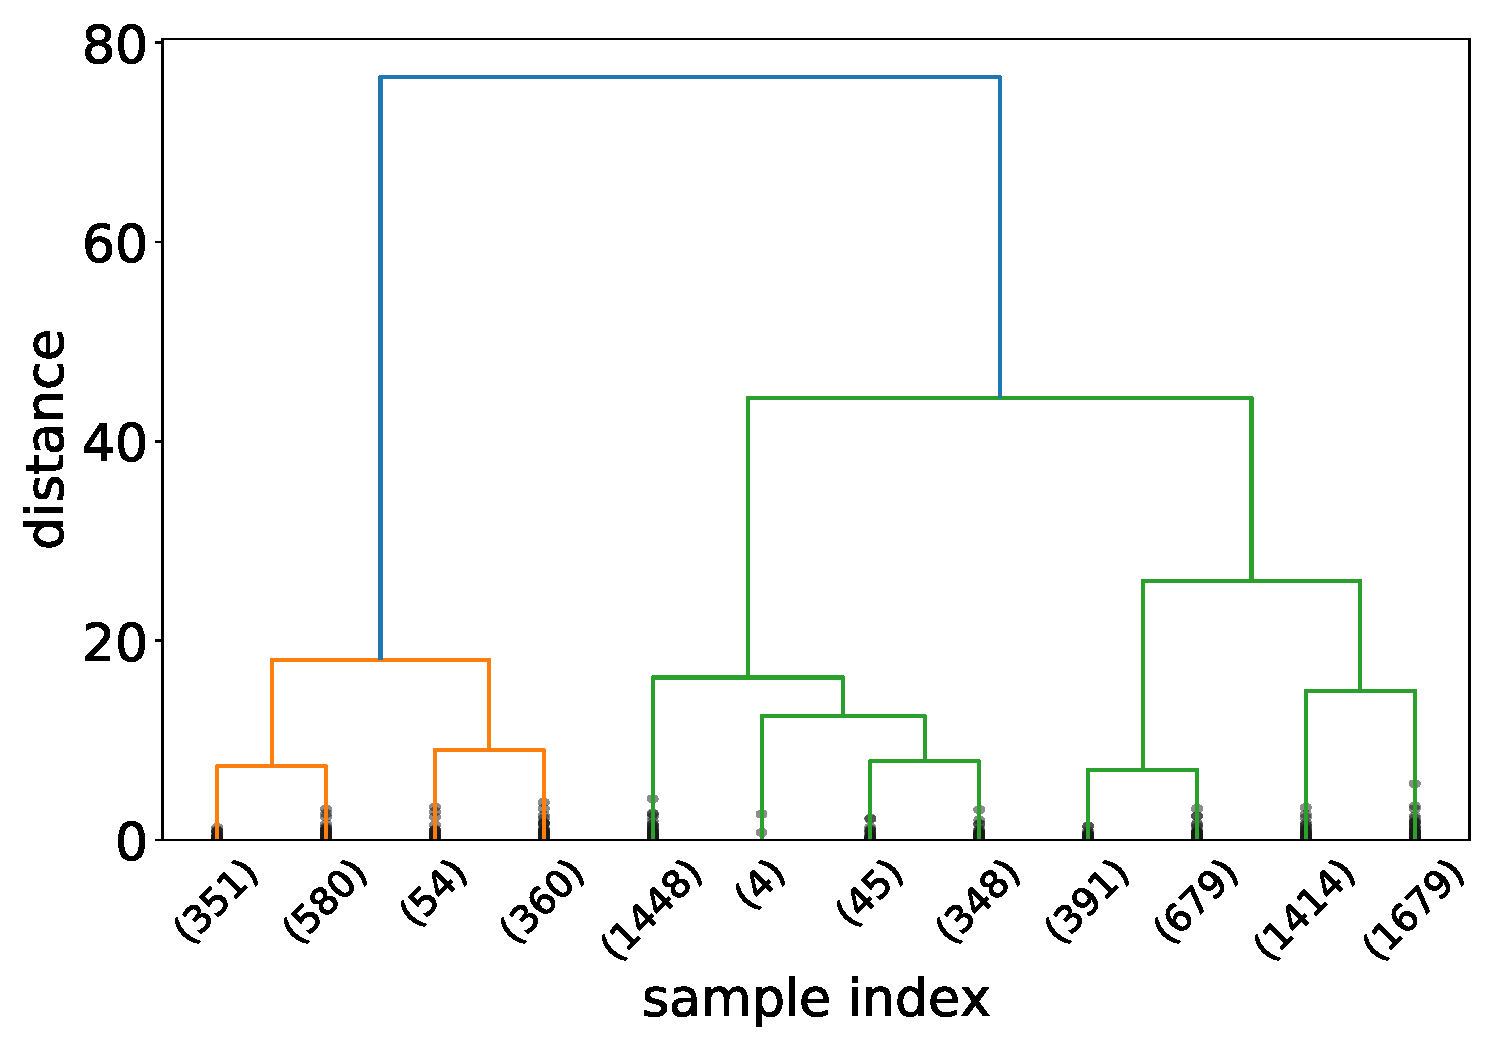
\includegraphics[width=0.9\linewidth]{Figs/Customer-Dendrograms.pdf}
    \caption{Costomer dendrogram...}
    \label{fig:dendrogram}
\end{figure}

\begin{figure}
	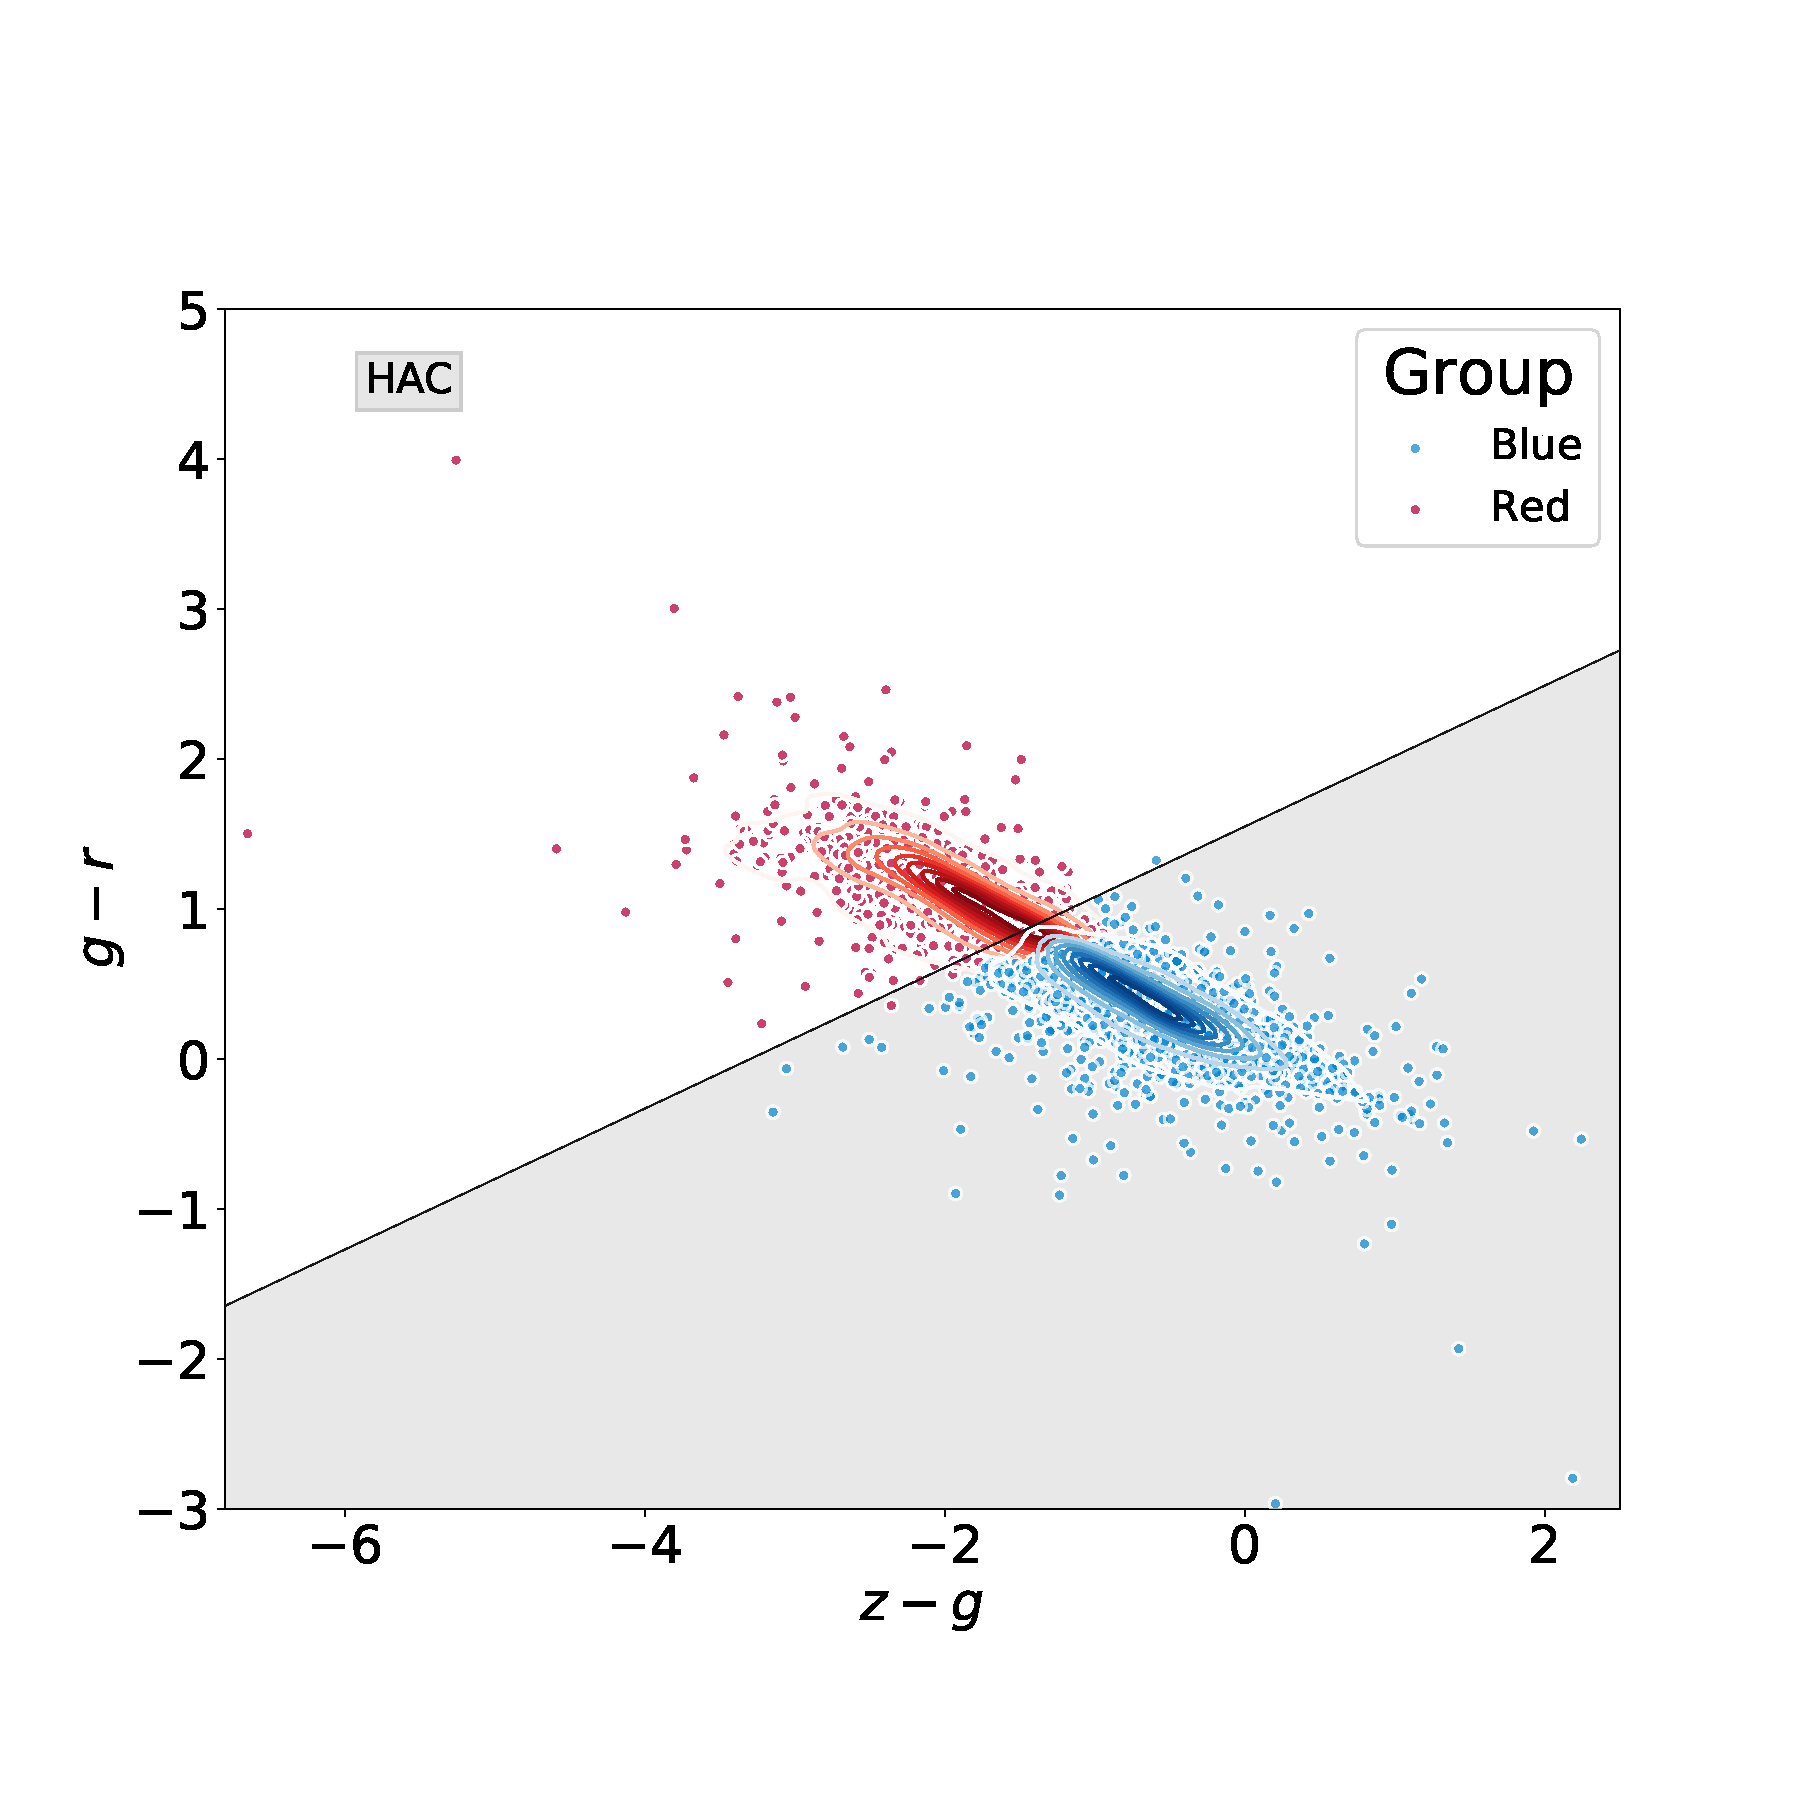
\includegraphics[width=0.9\linewidth]{Figs/blued-red-hierarchical.pdf}
    \caption{Costomer dendrogram...}
    \label{fig:hierar}
\end{figure}

\begin{figure*}
\centering
\begin{tabular}{l l}
  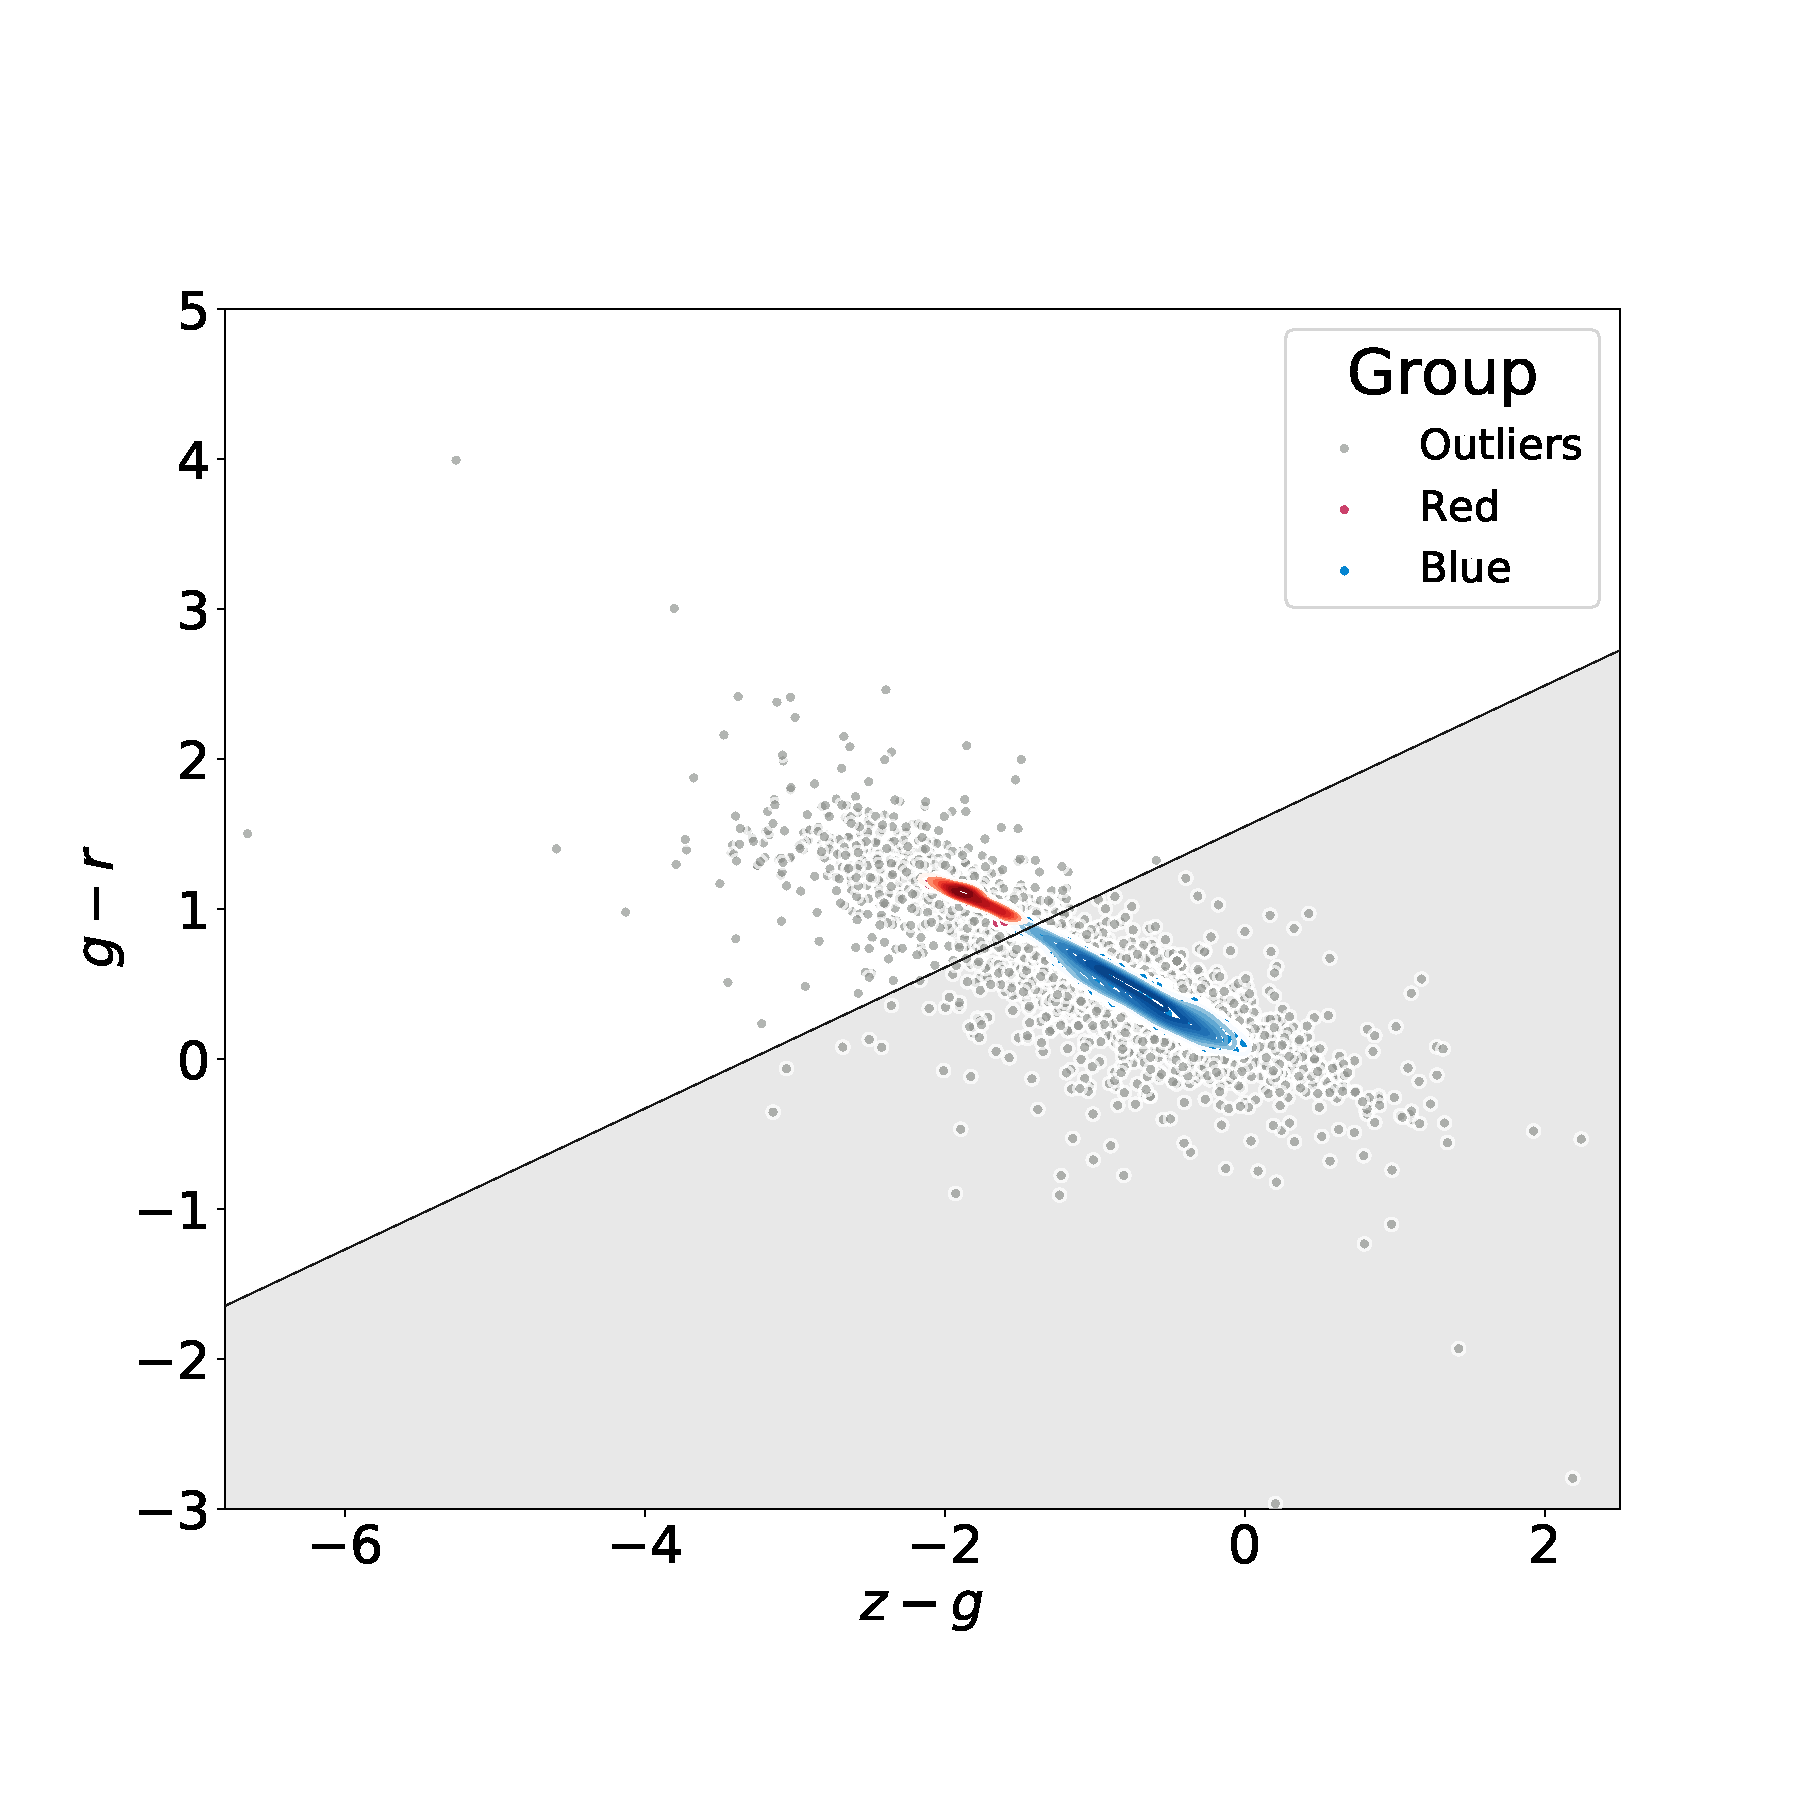
\includegraphics[width=0.5\linewidth, trim=10 10 5 8, clip]{Figs/blued-red-hdbscan.pdf}
   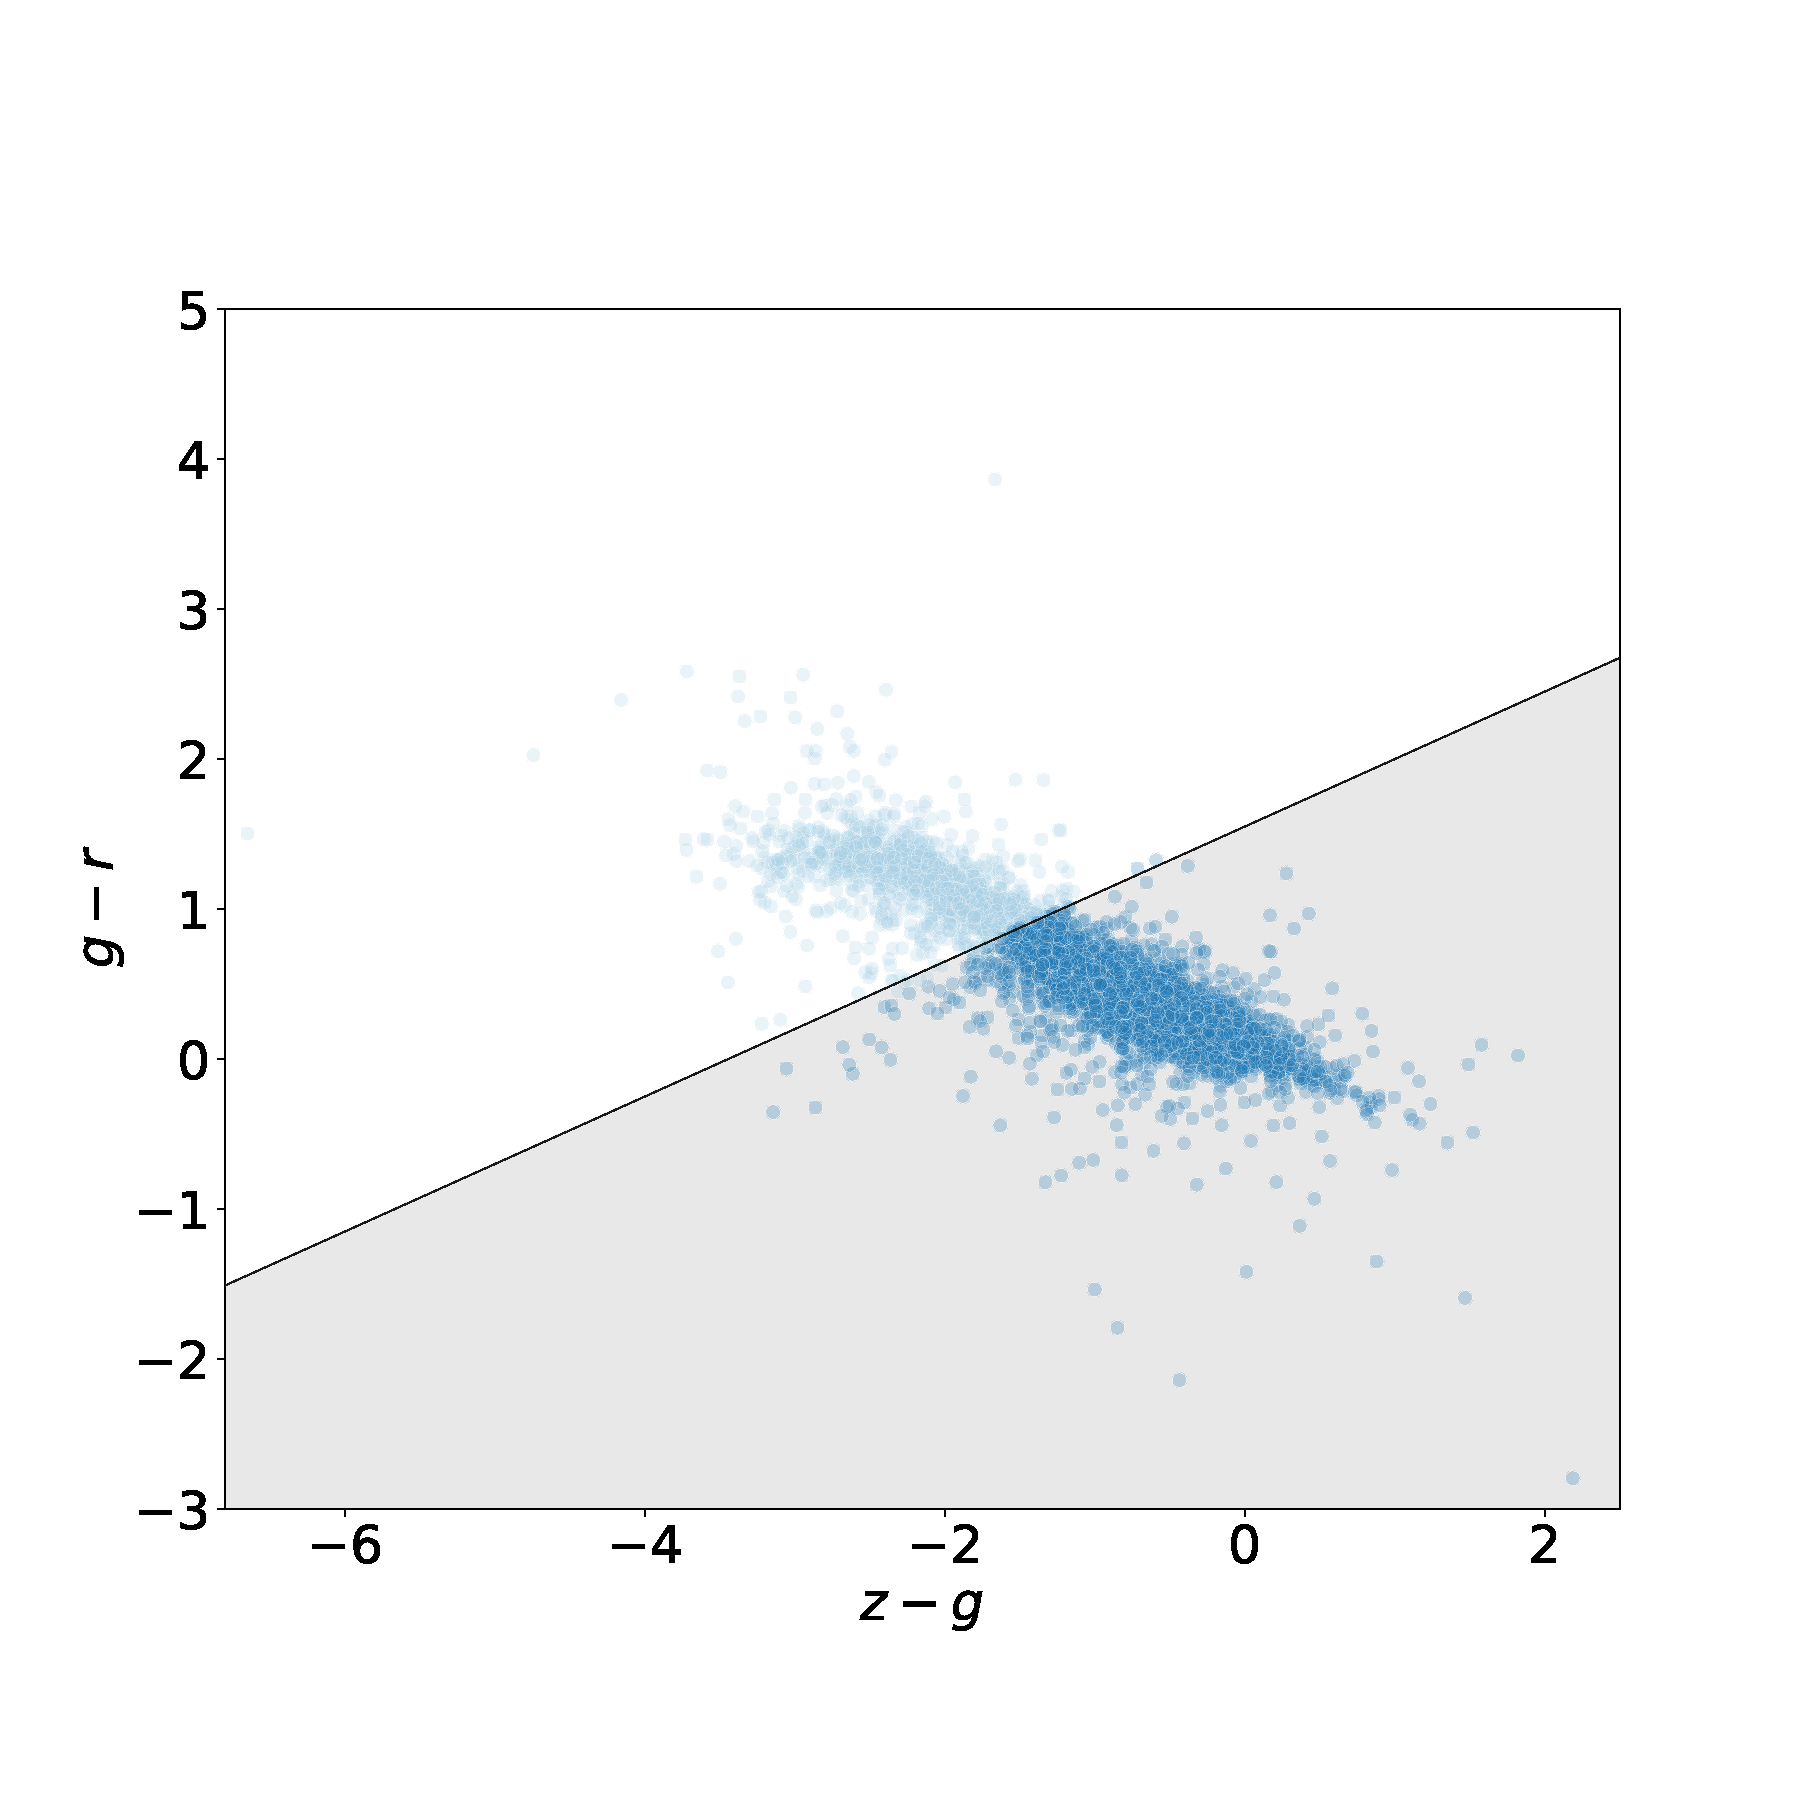
\includegraphics[width=0.5\linewidth, trim=10 10 5 8. clip]{Figs/blued-red-hdbscan-soft.pdf}
  \end{tabular}  
  \caption{New color-color diagram to separate the blue objects from the red ones.}
\label{fig:hdbscan}
\end{figure*}


\begin{figure*}
  \setlength\tabcolsep{0pt}
  \setkeys{Gin}{width=0.5\linewidth}
  \begin{tabular}{ll}
    (a) & (b) \\
    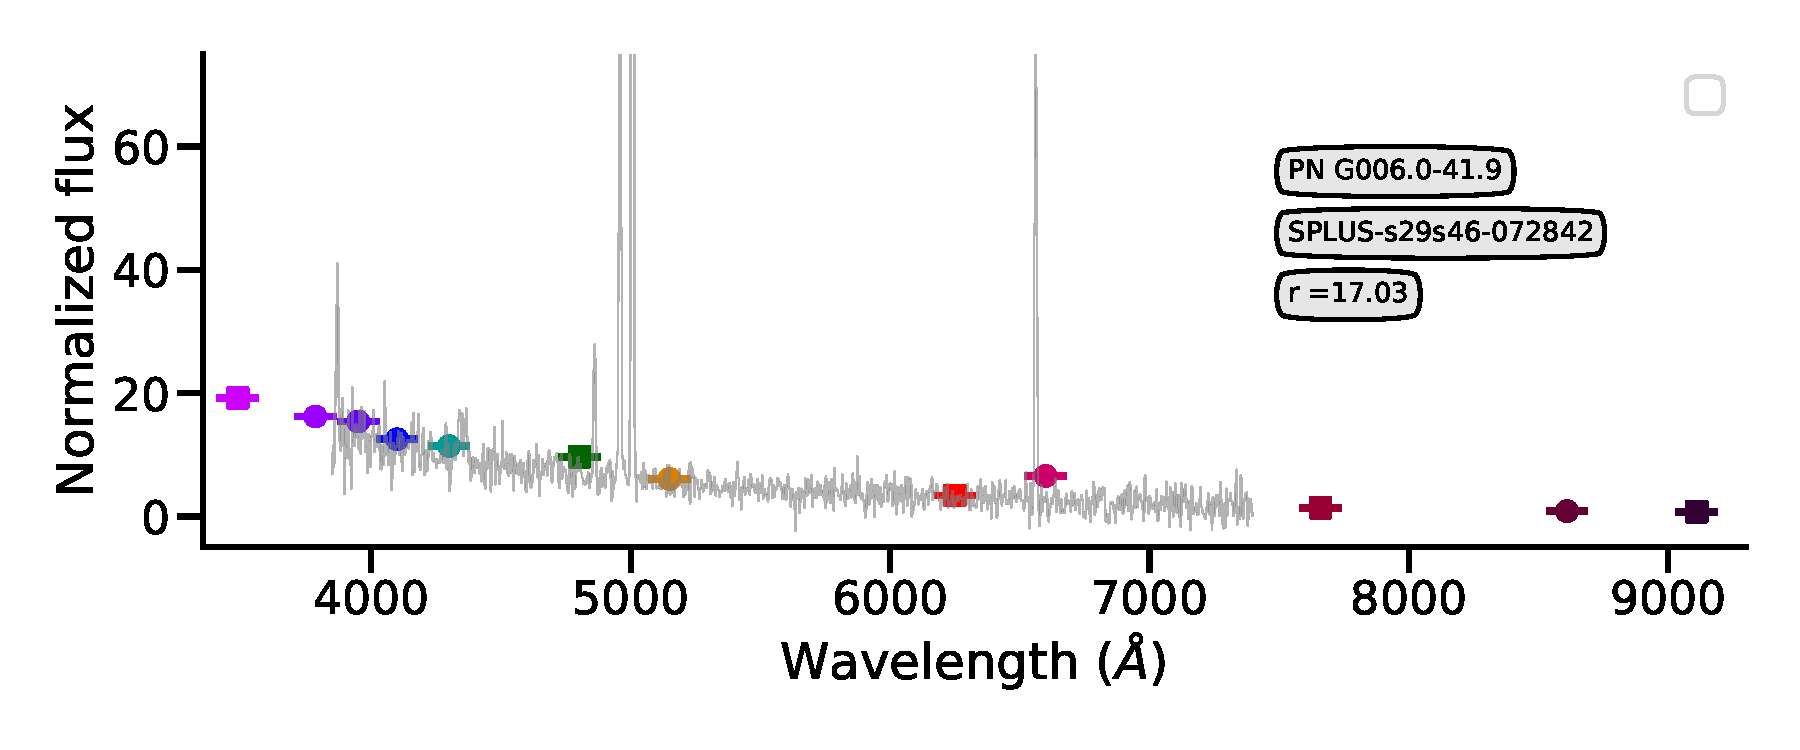
\includegraphics[trim=10 0 10 20, clip]{Figs/StenholmAcker_pn_g006_0-41_9_id176-SPLUS-s29s46-072842.pdf} & 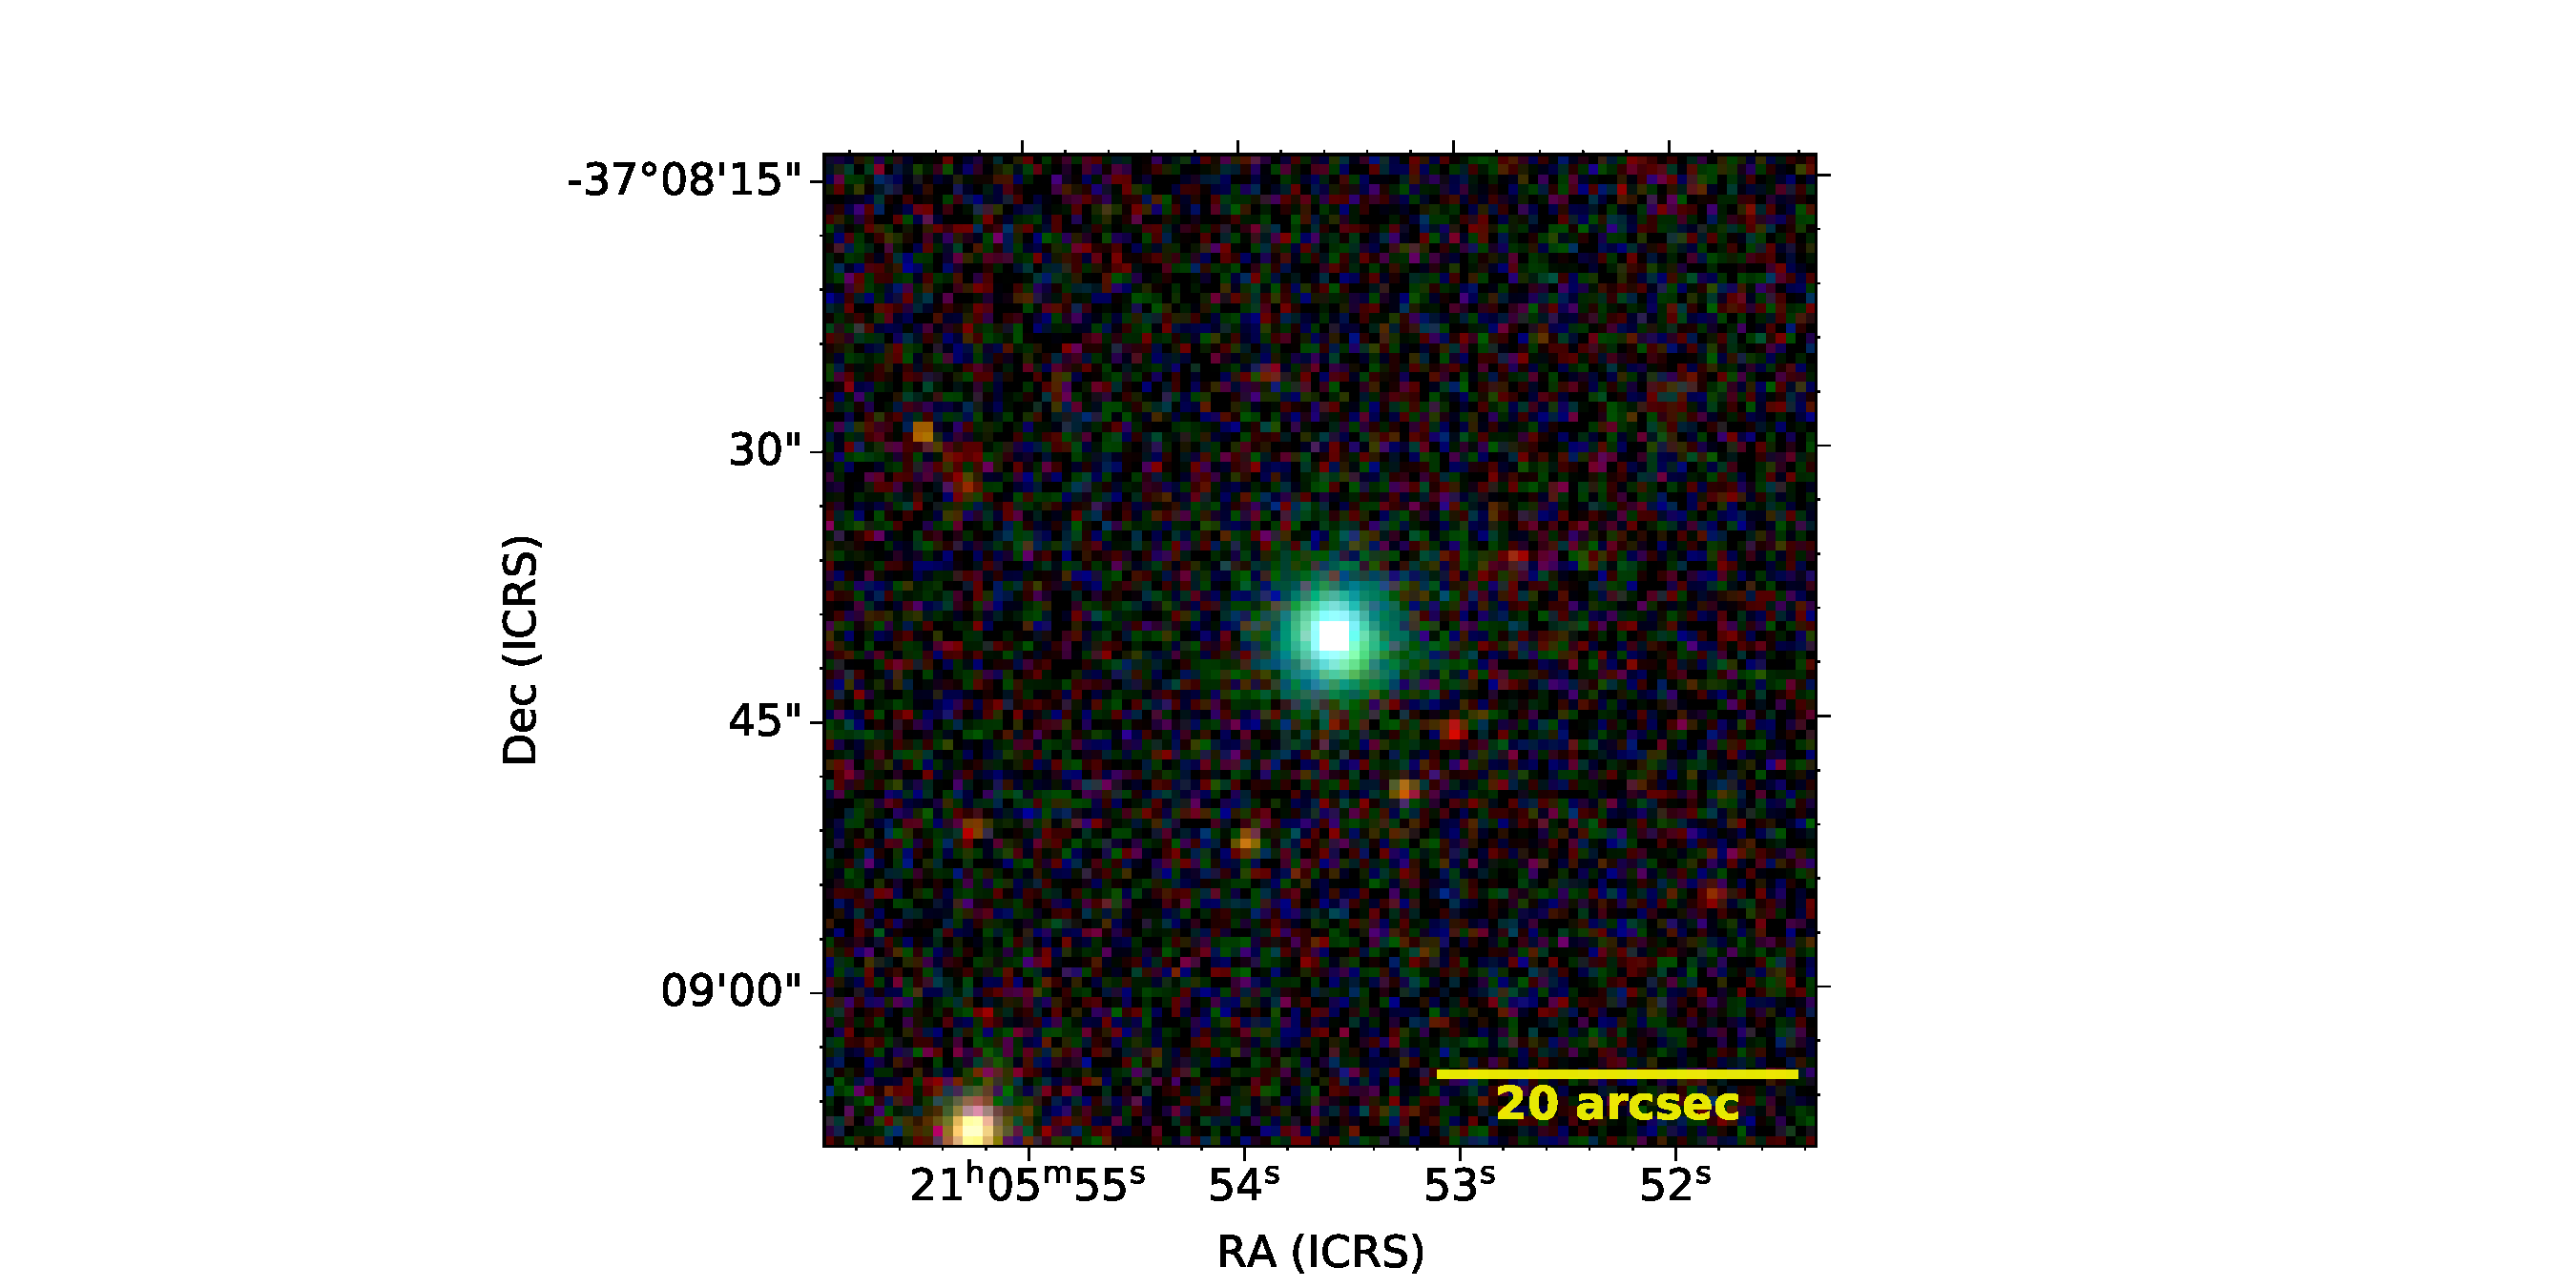
\includegraphics[width=0.4\linewidth, trim=10 0 10 20, clip]{Figs/PNG006_316-37_100_r.pdf} \\
     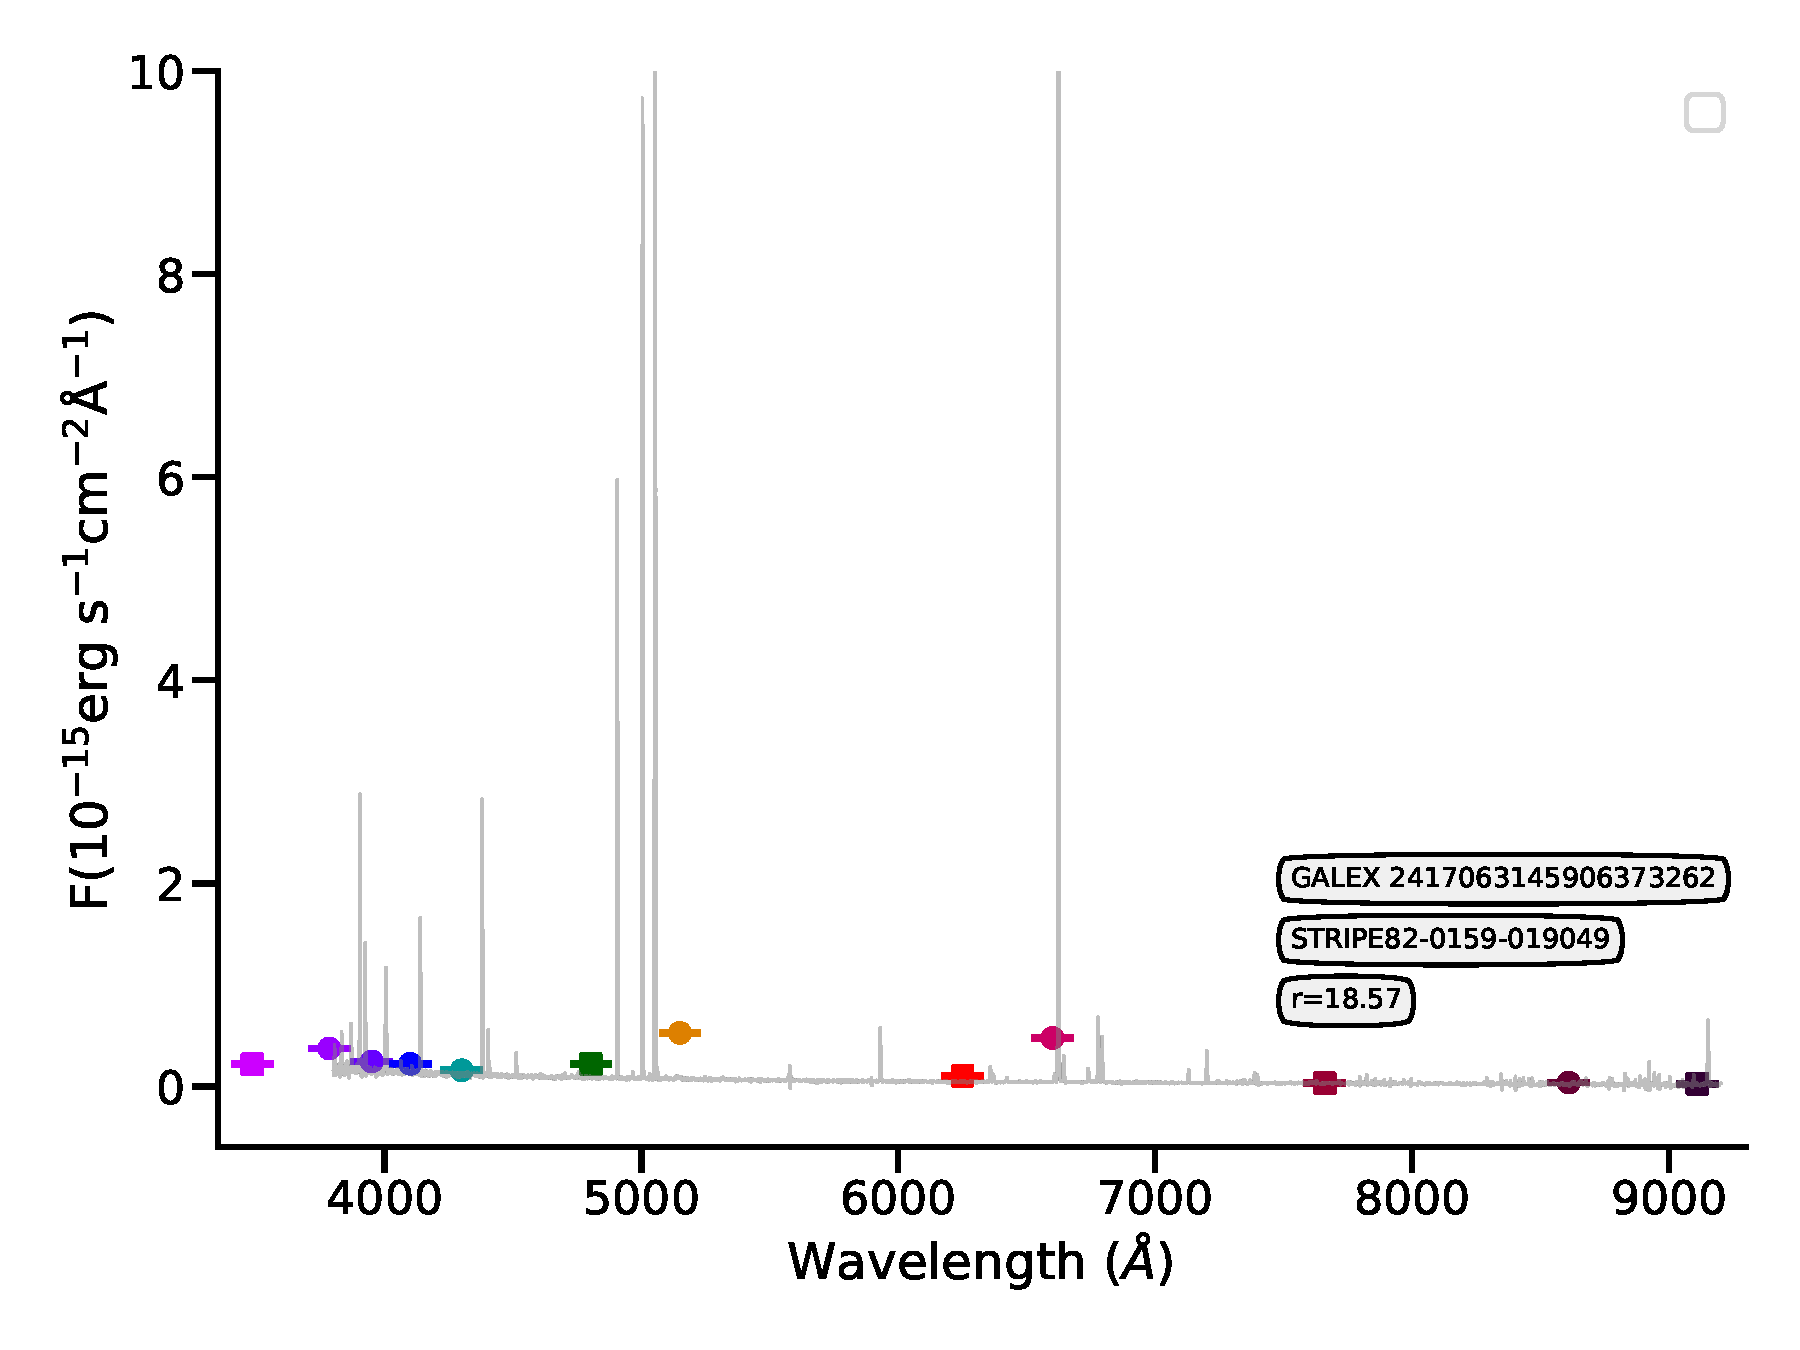
\includegraphics[trim=10 0 10 20, clip]{Figs/spec-0680-52200-0153-STRIPE82-0159-019049.pdf} & 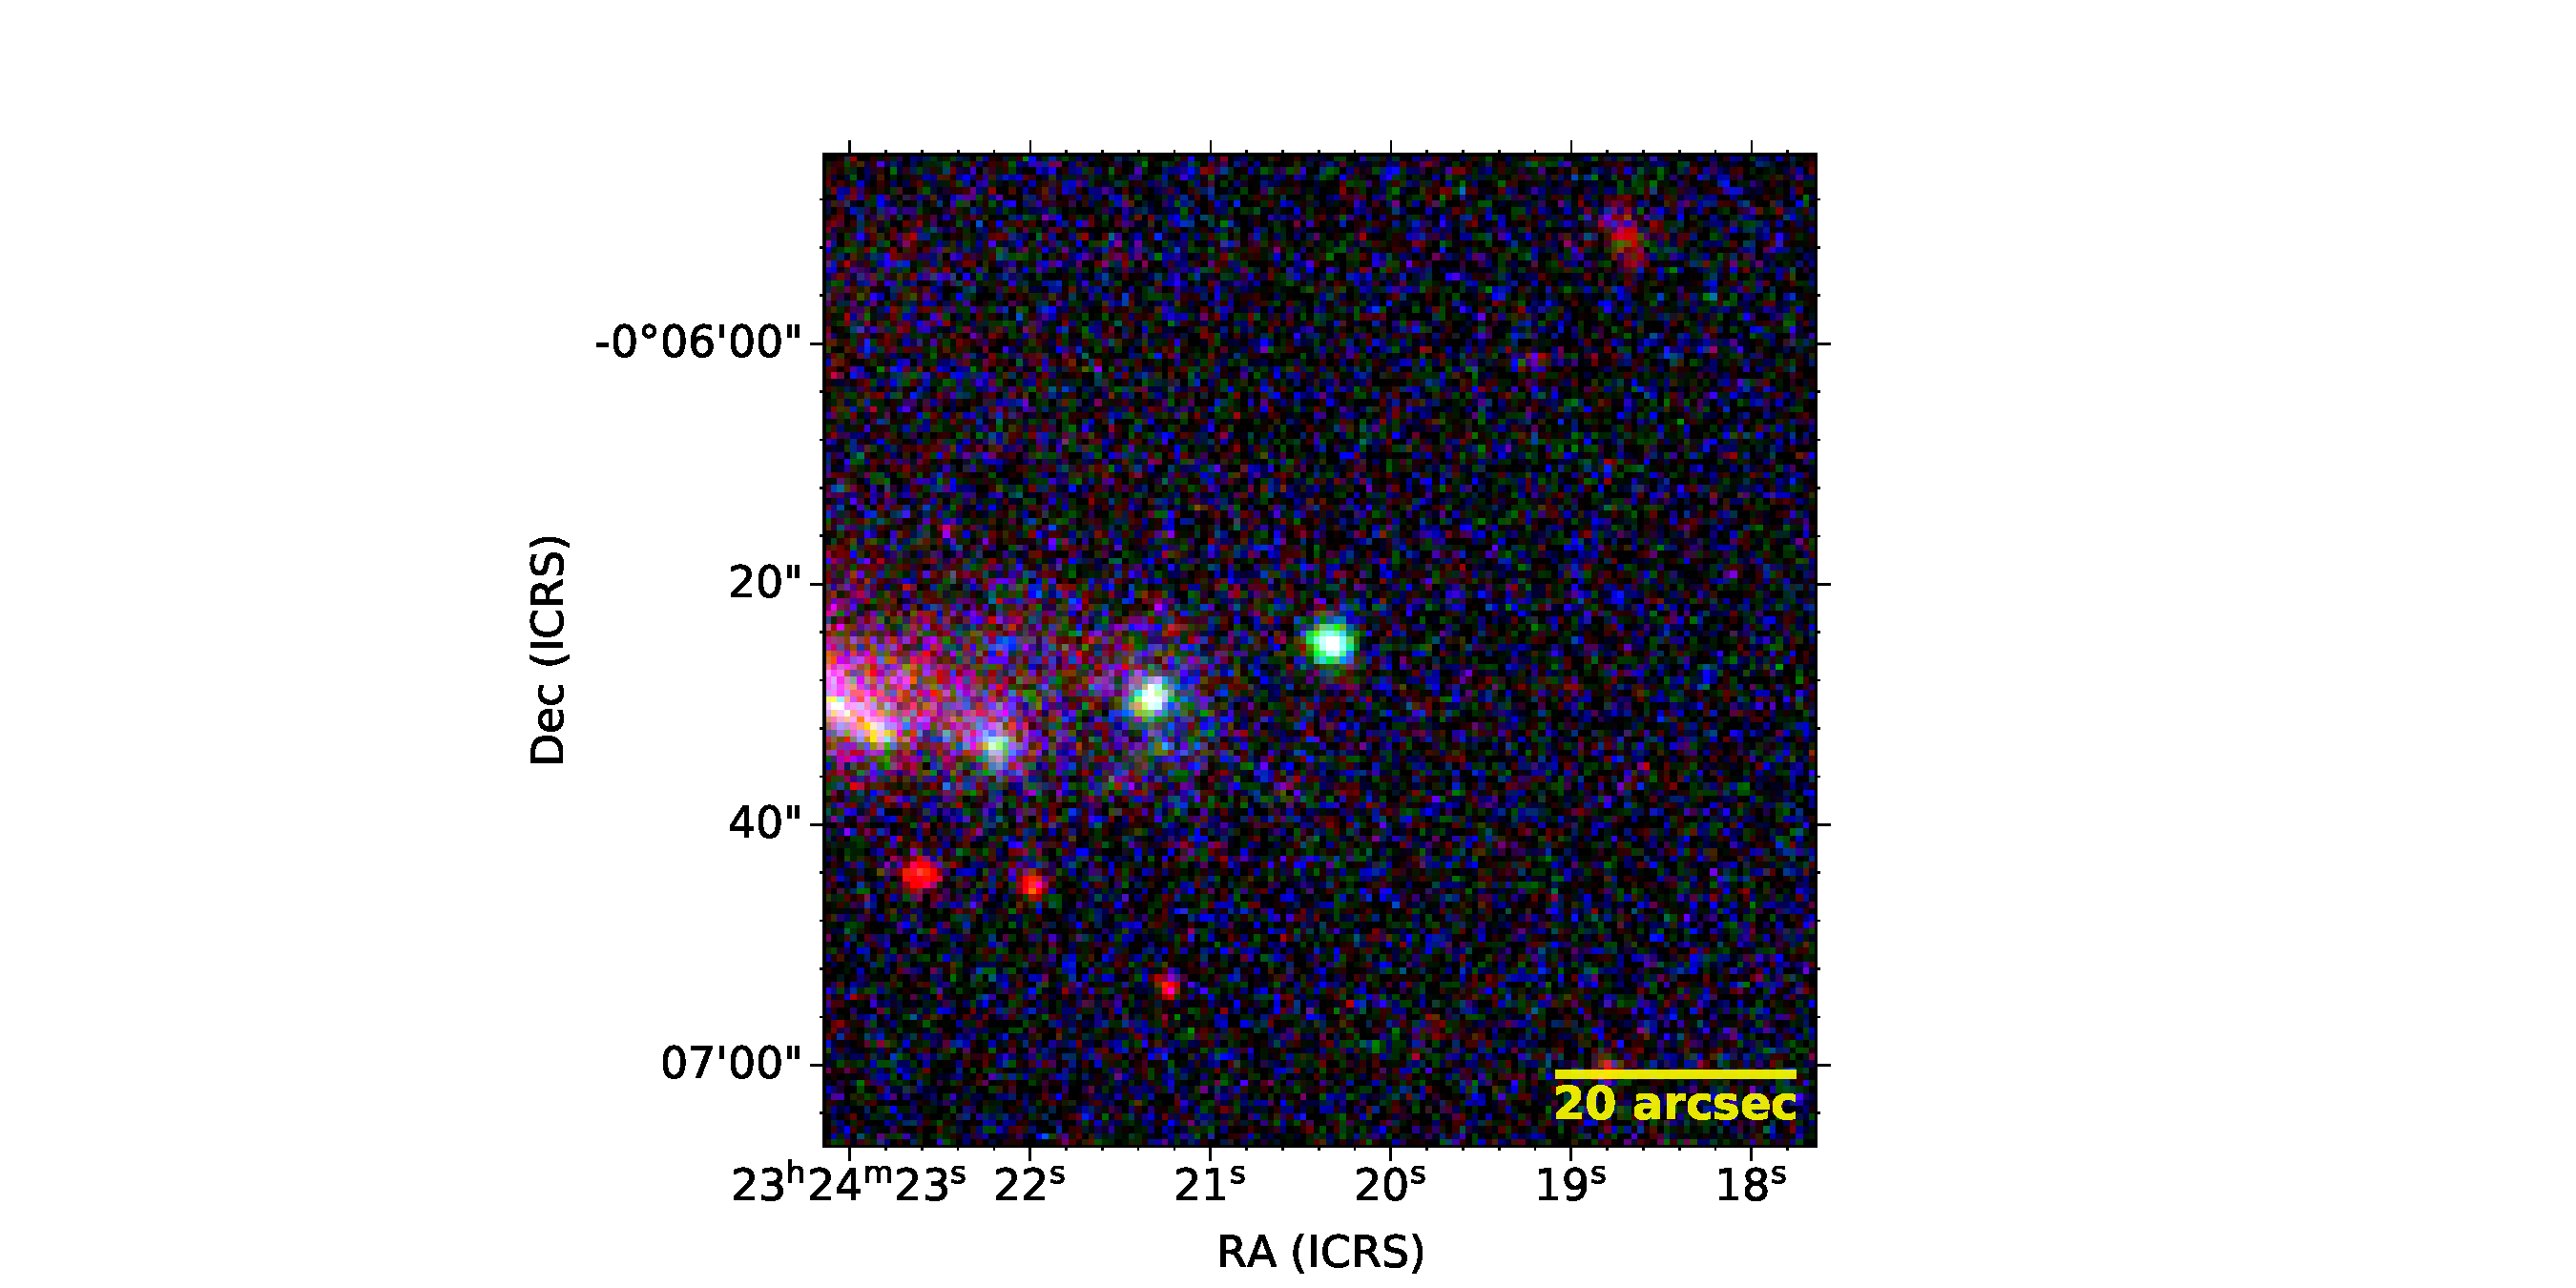
\includegraphics[width=0.4\linewidth, trim=10 0 10 20, clip]{Figs/GALEX24170_351-0_150_r.pdf} \\
    (c) & (d) \\
    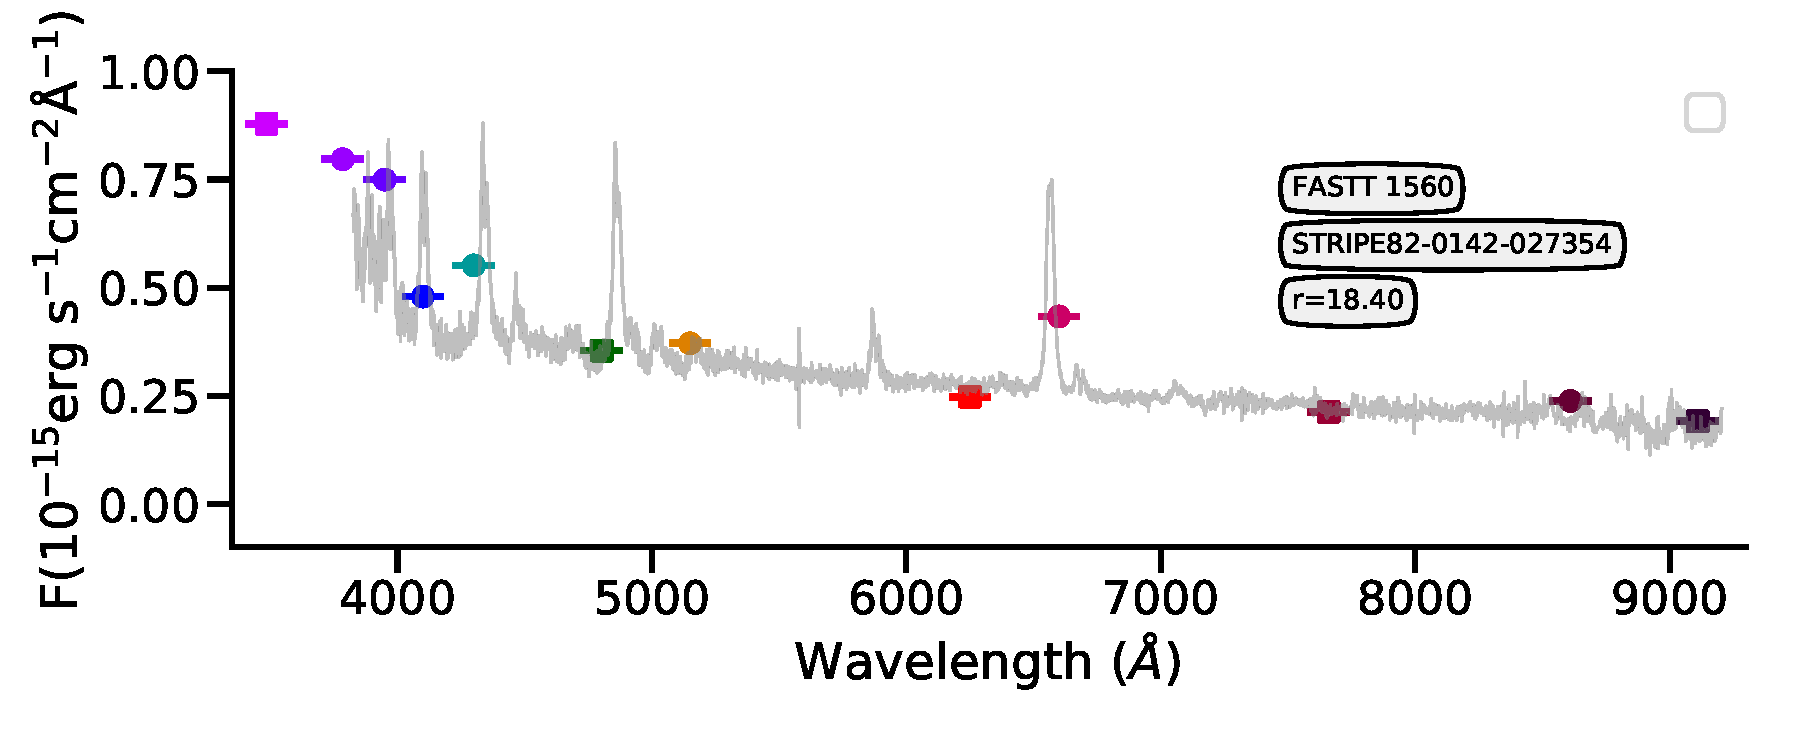
\includegraphics[trim=10 0 10 20, clip]{Figs/spec-0376-52143-0631-STRIPE82-0142-027354.pdf} & 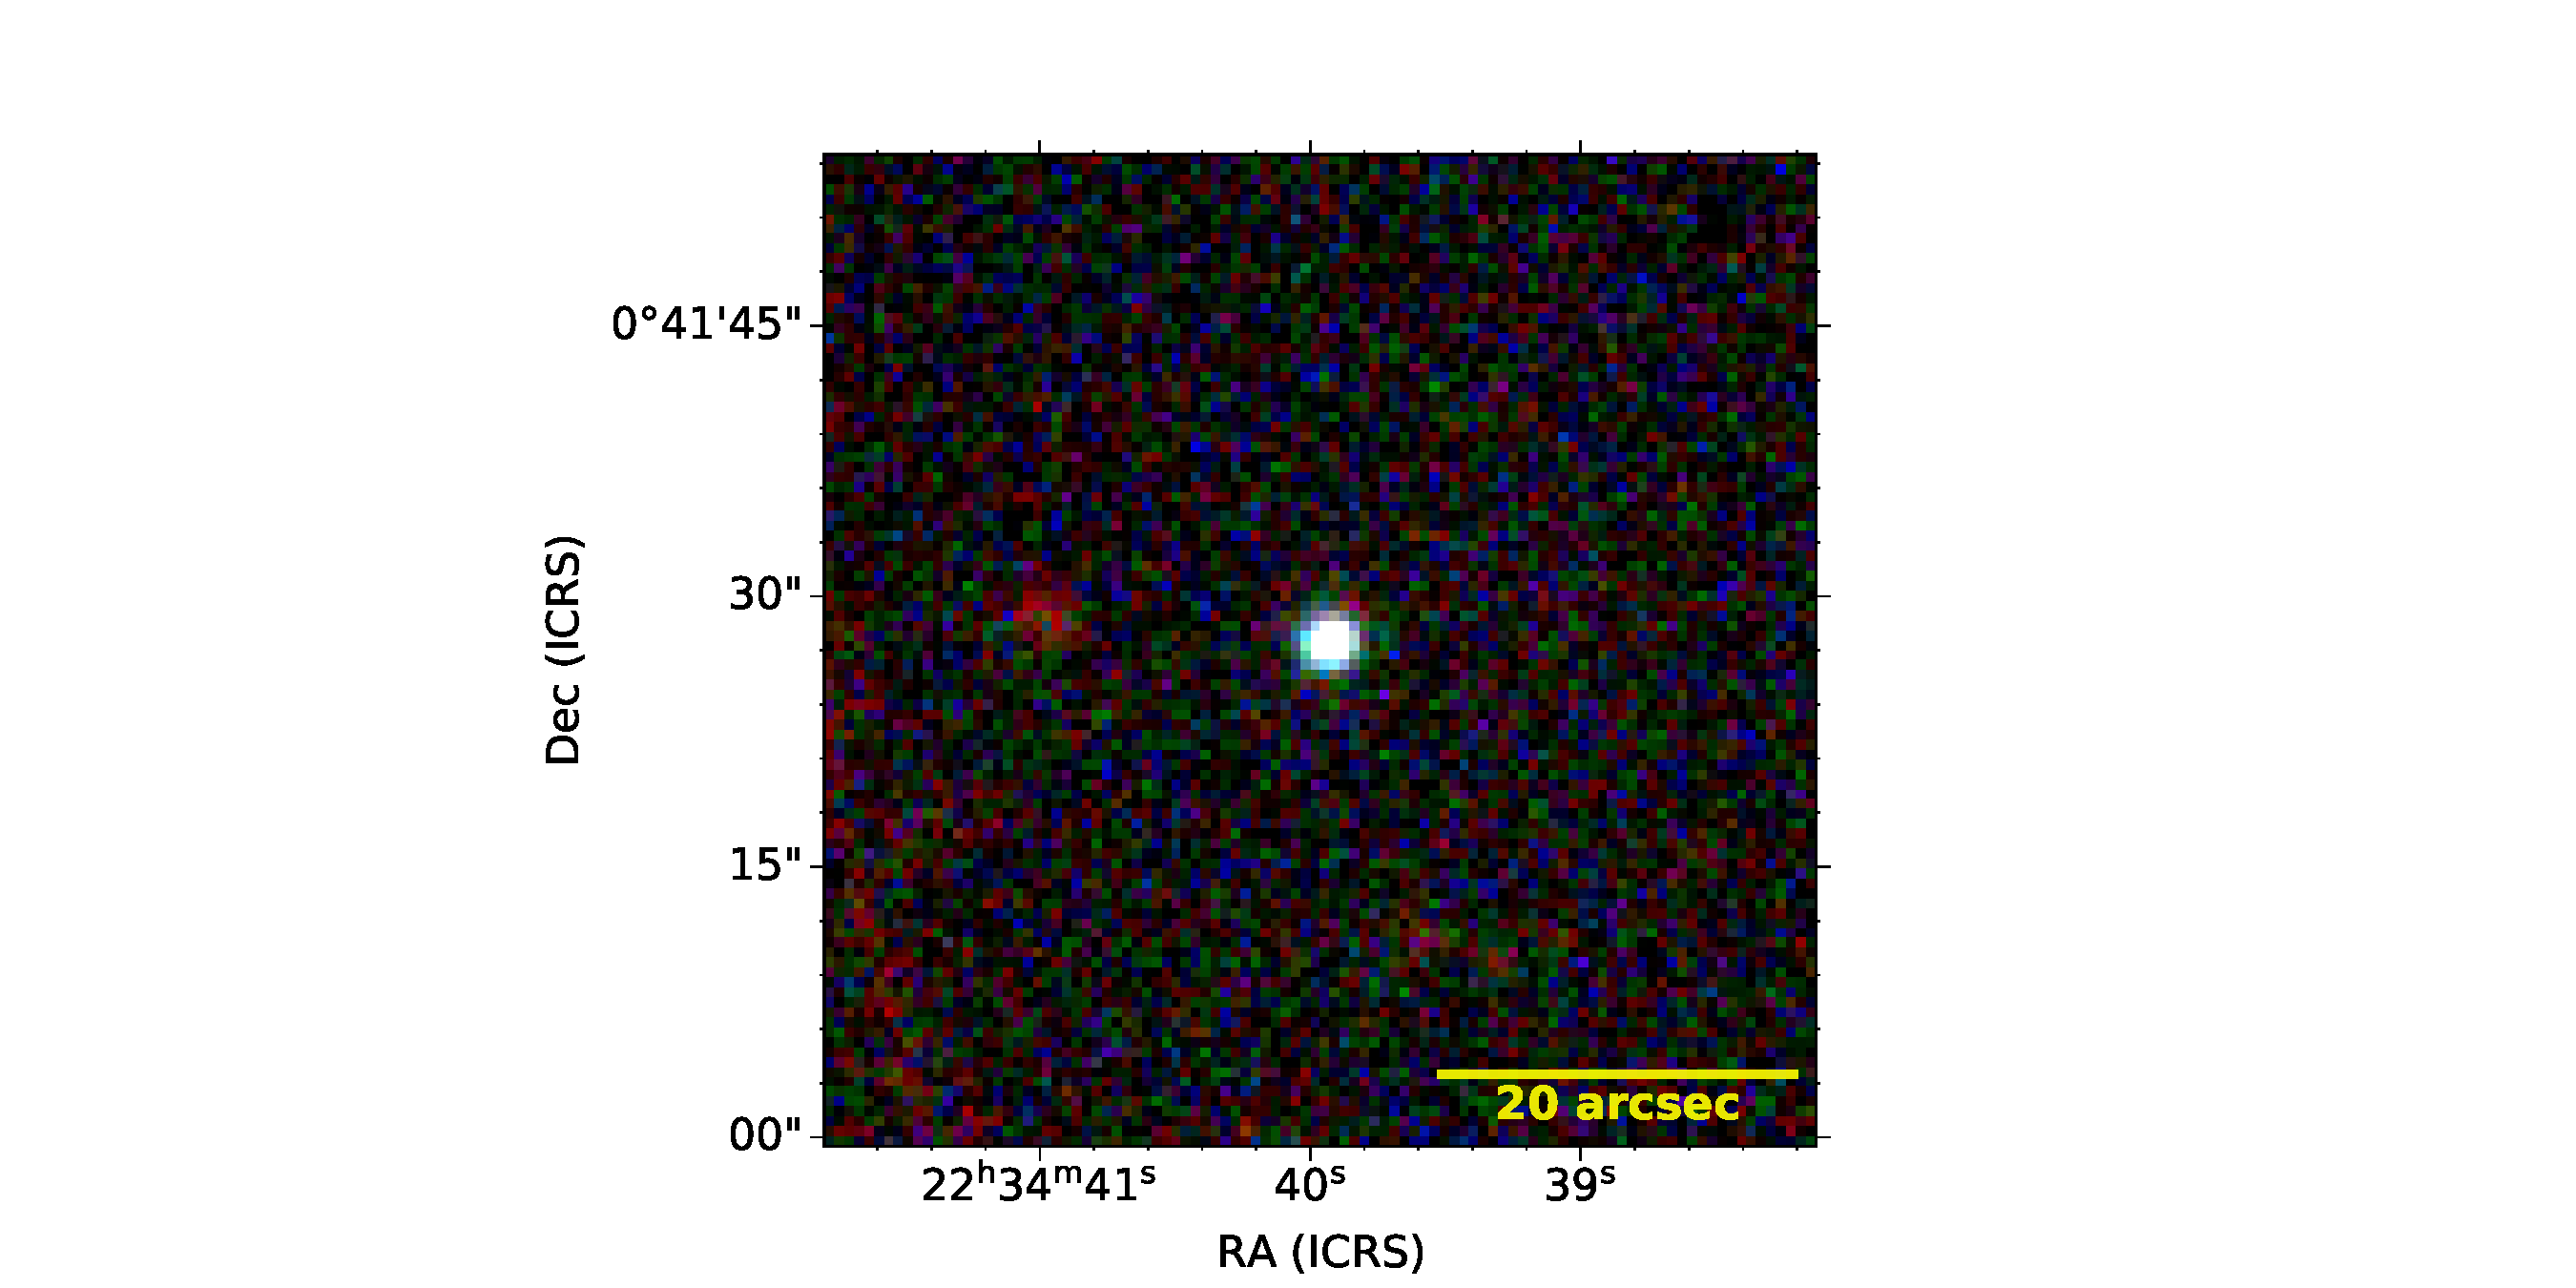
\includegraphics[width=0.4\linewidth, trim=10 0 10 20, clip]{Figs/FASTT1560_338-0_100_r.pdf} \\
     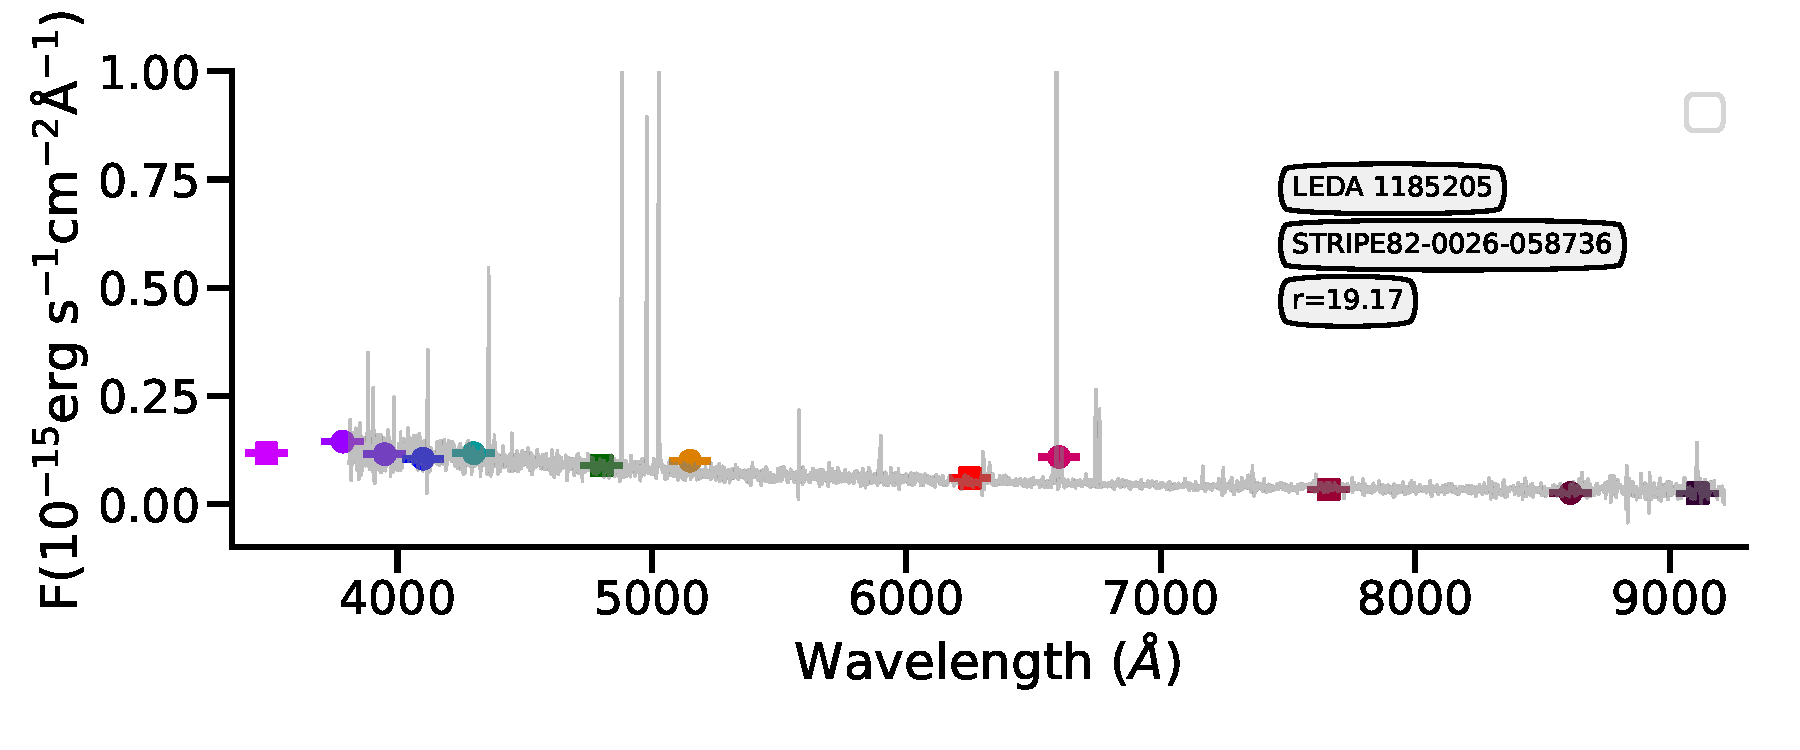
\includegraphics[trim=10 0 10 20, clip]{Figs/spec-0397-51794-0336-STRIPE82-0026-058736.pdf} & 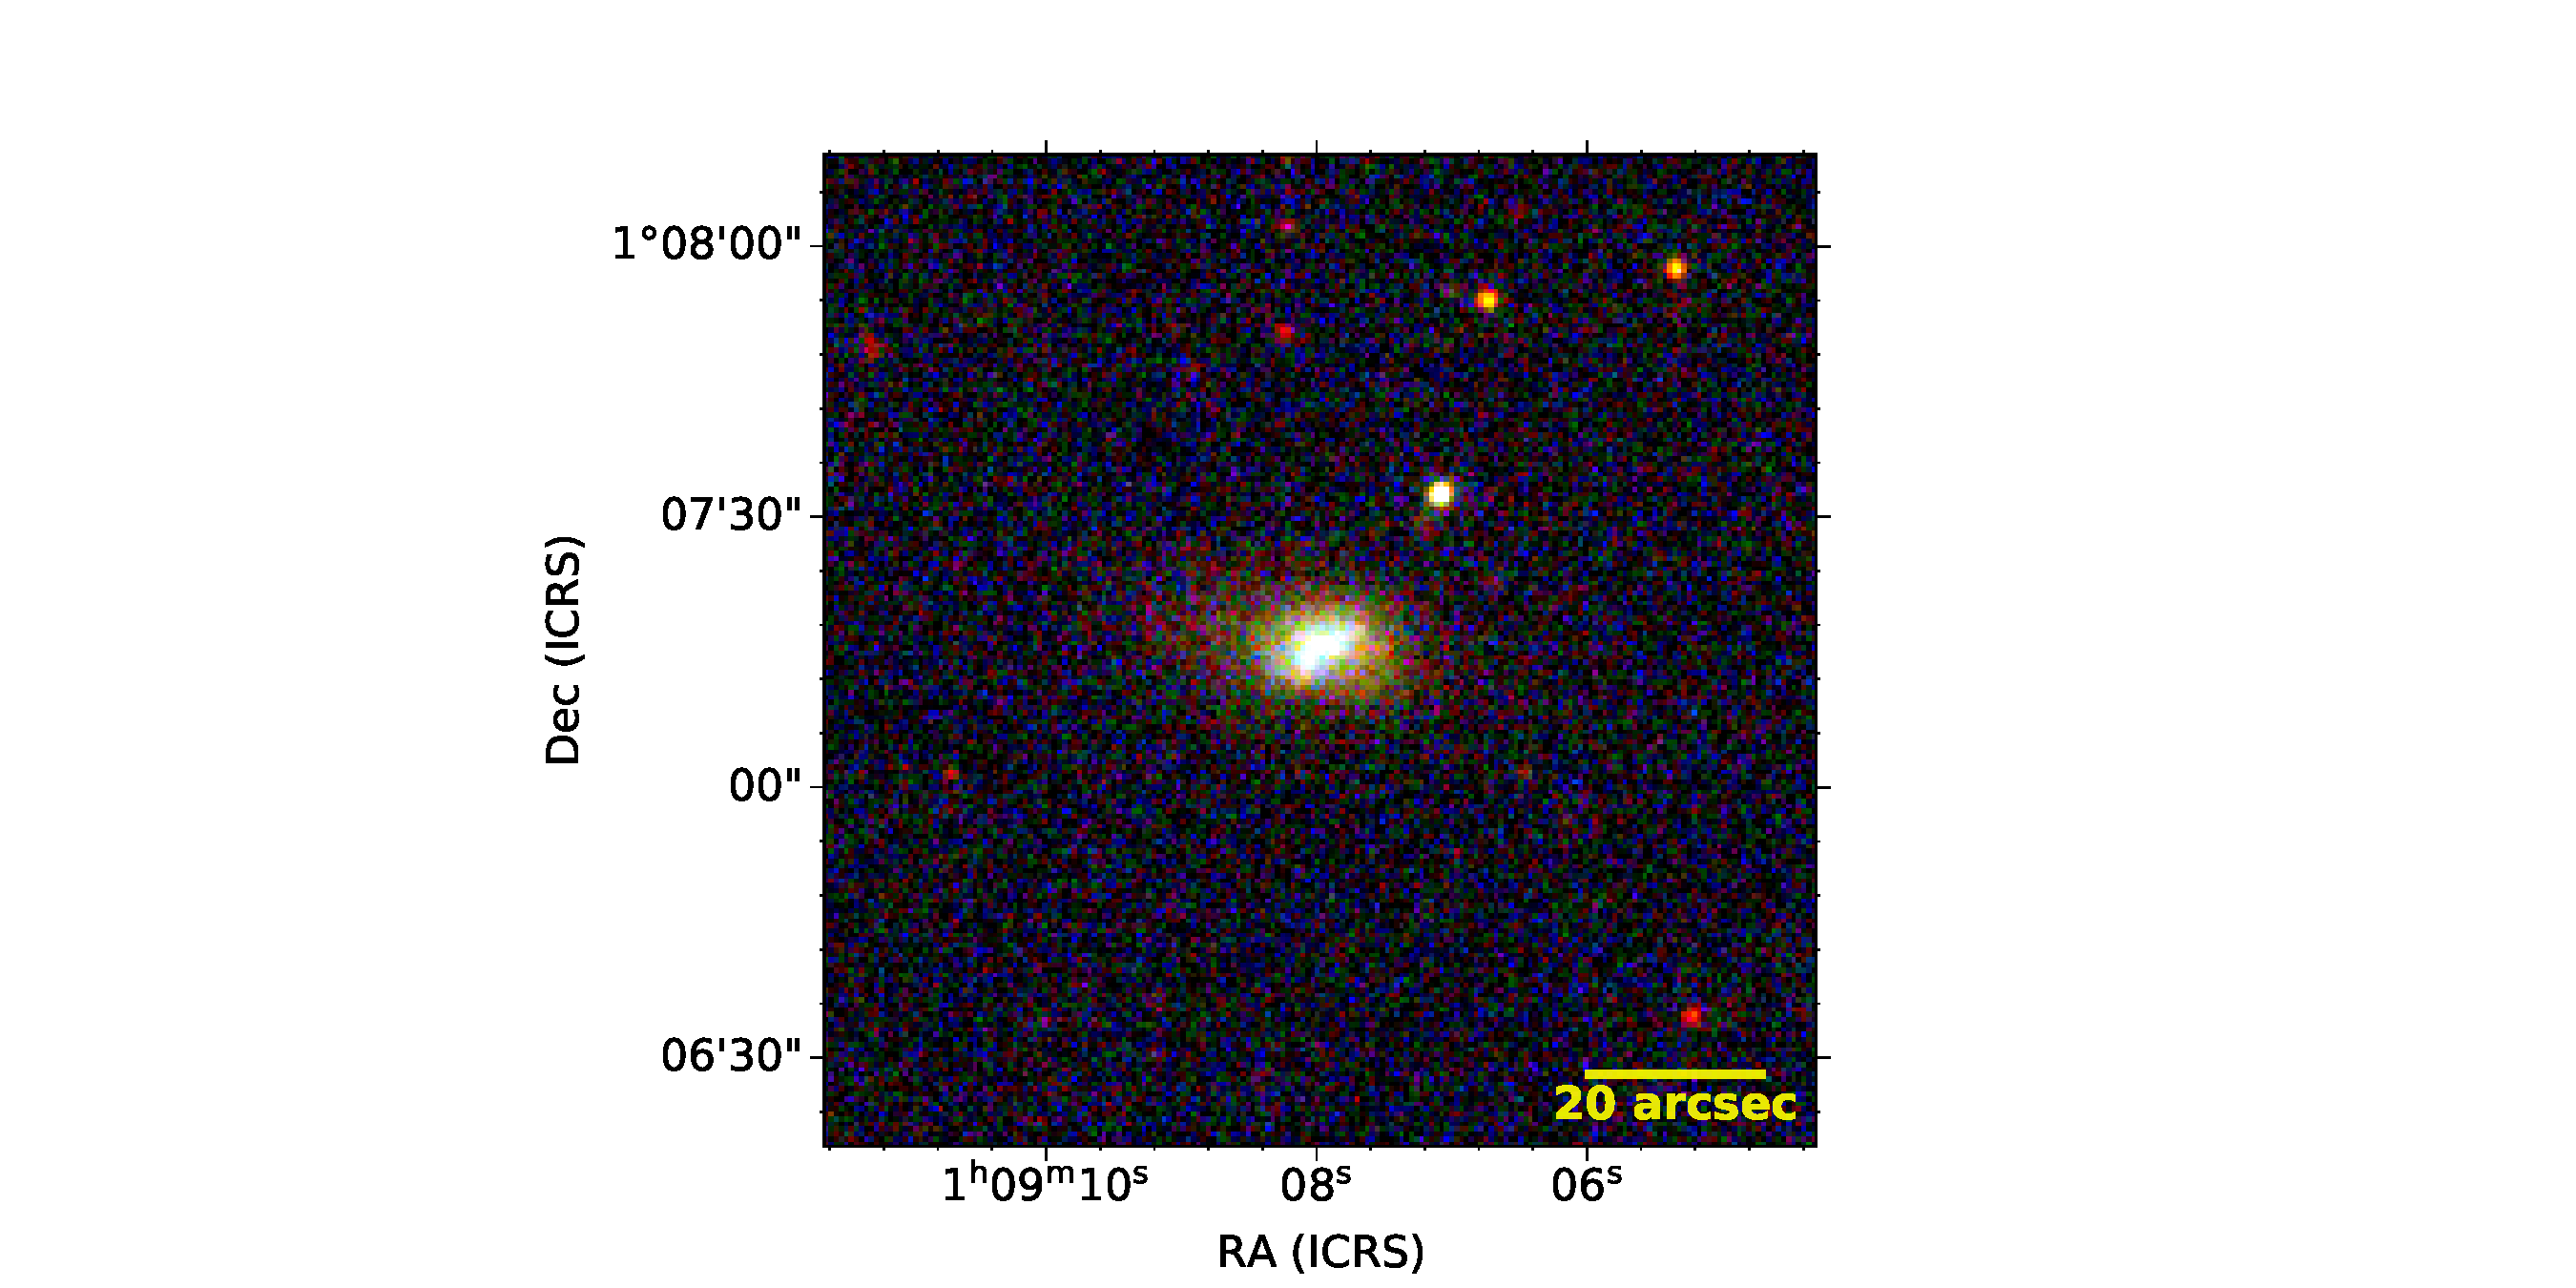
\includegraphics[width=0.4\linewidth, trim=10 0 10 20, clip]{Figs/LEDA1185205_17-1_200_r.pdf} \\
     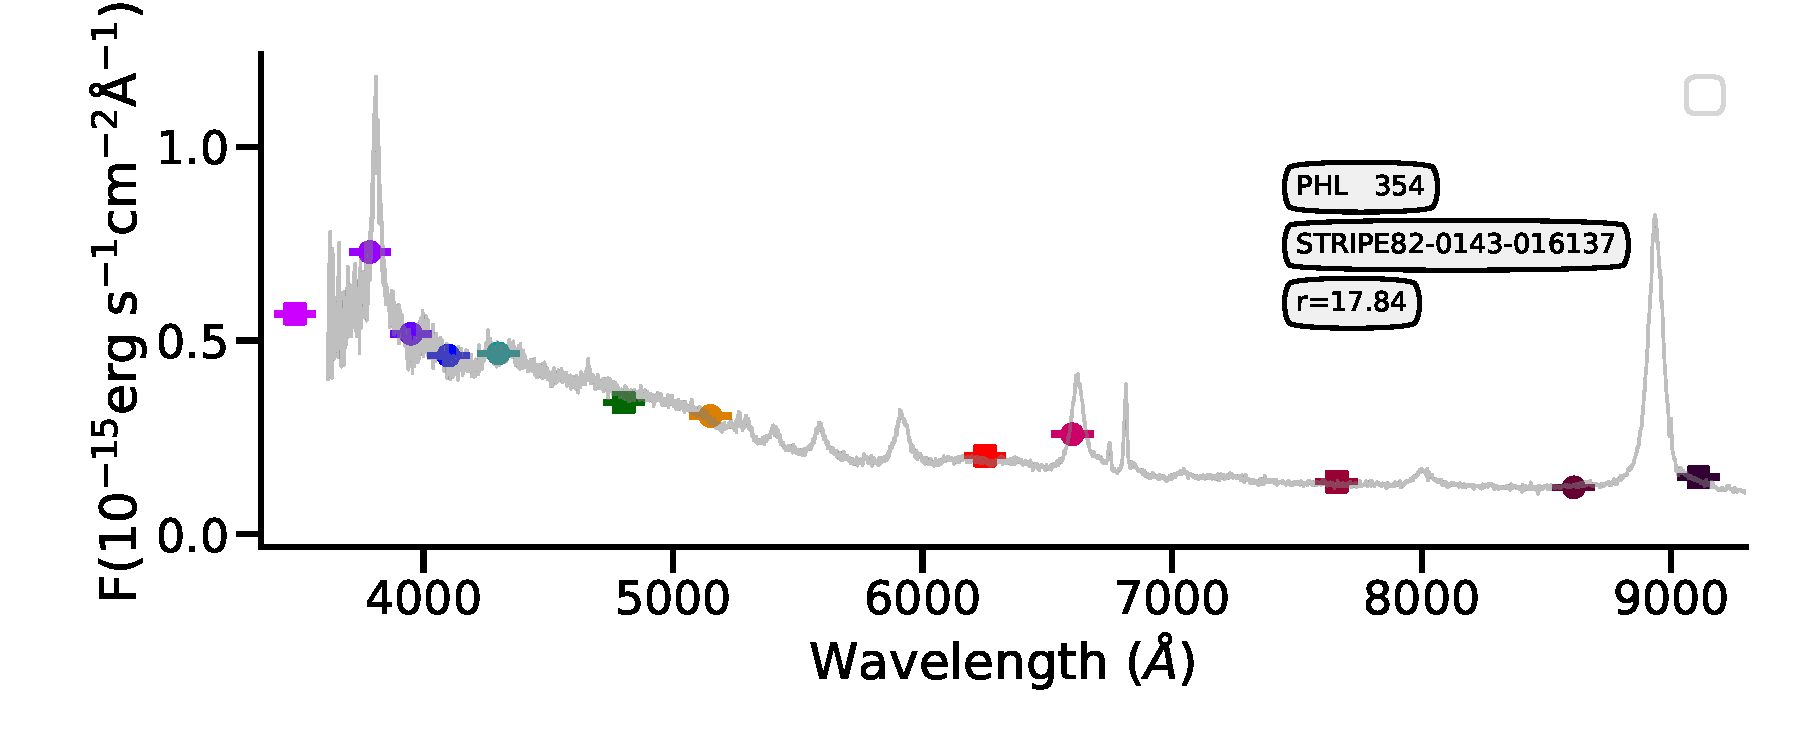
\includegraphics[trim=10 0 10 20, clip]{Figs/spec-9217-57934-0839-STRIPE82-0143-016137.pdf} & 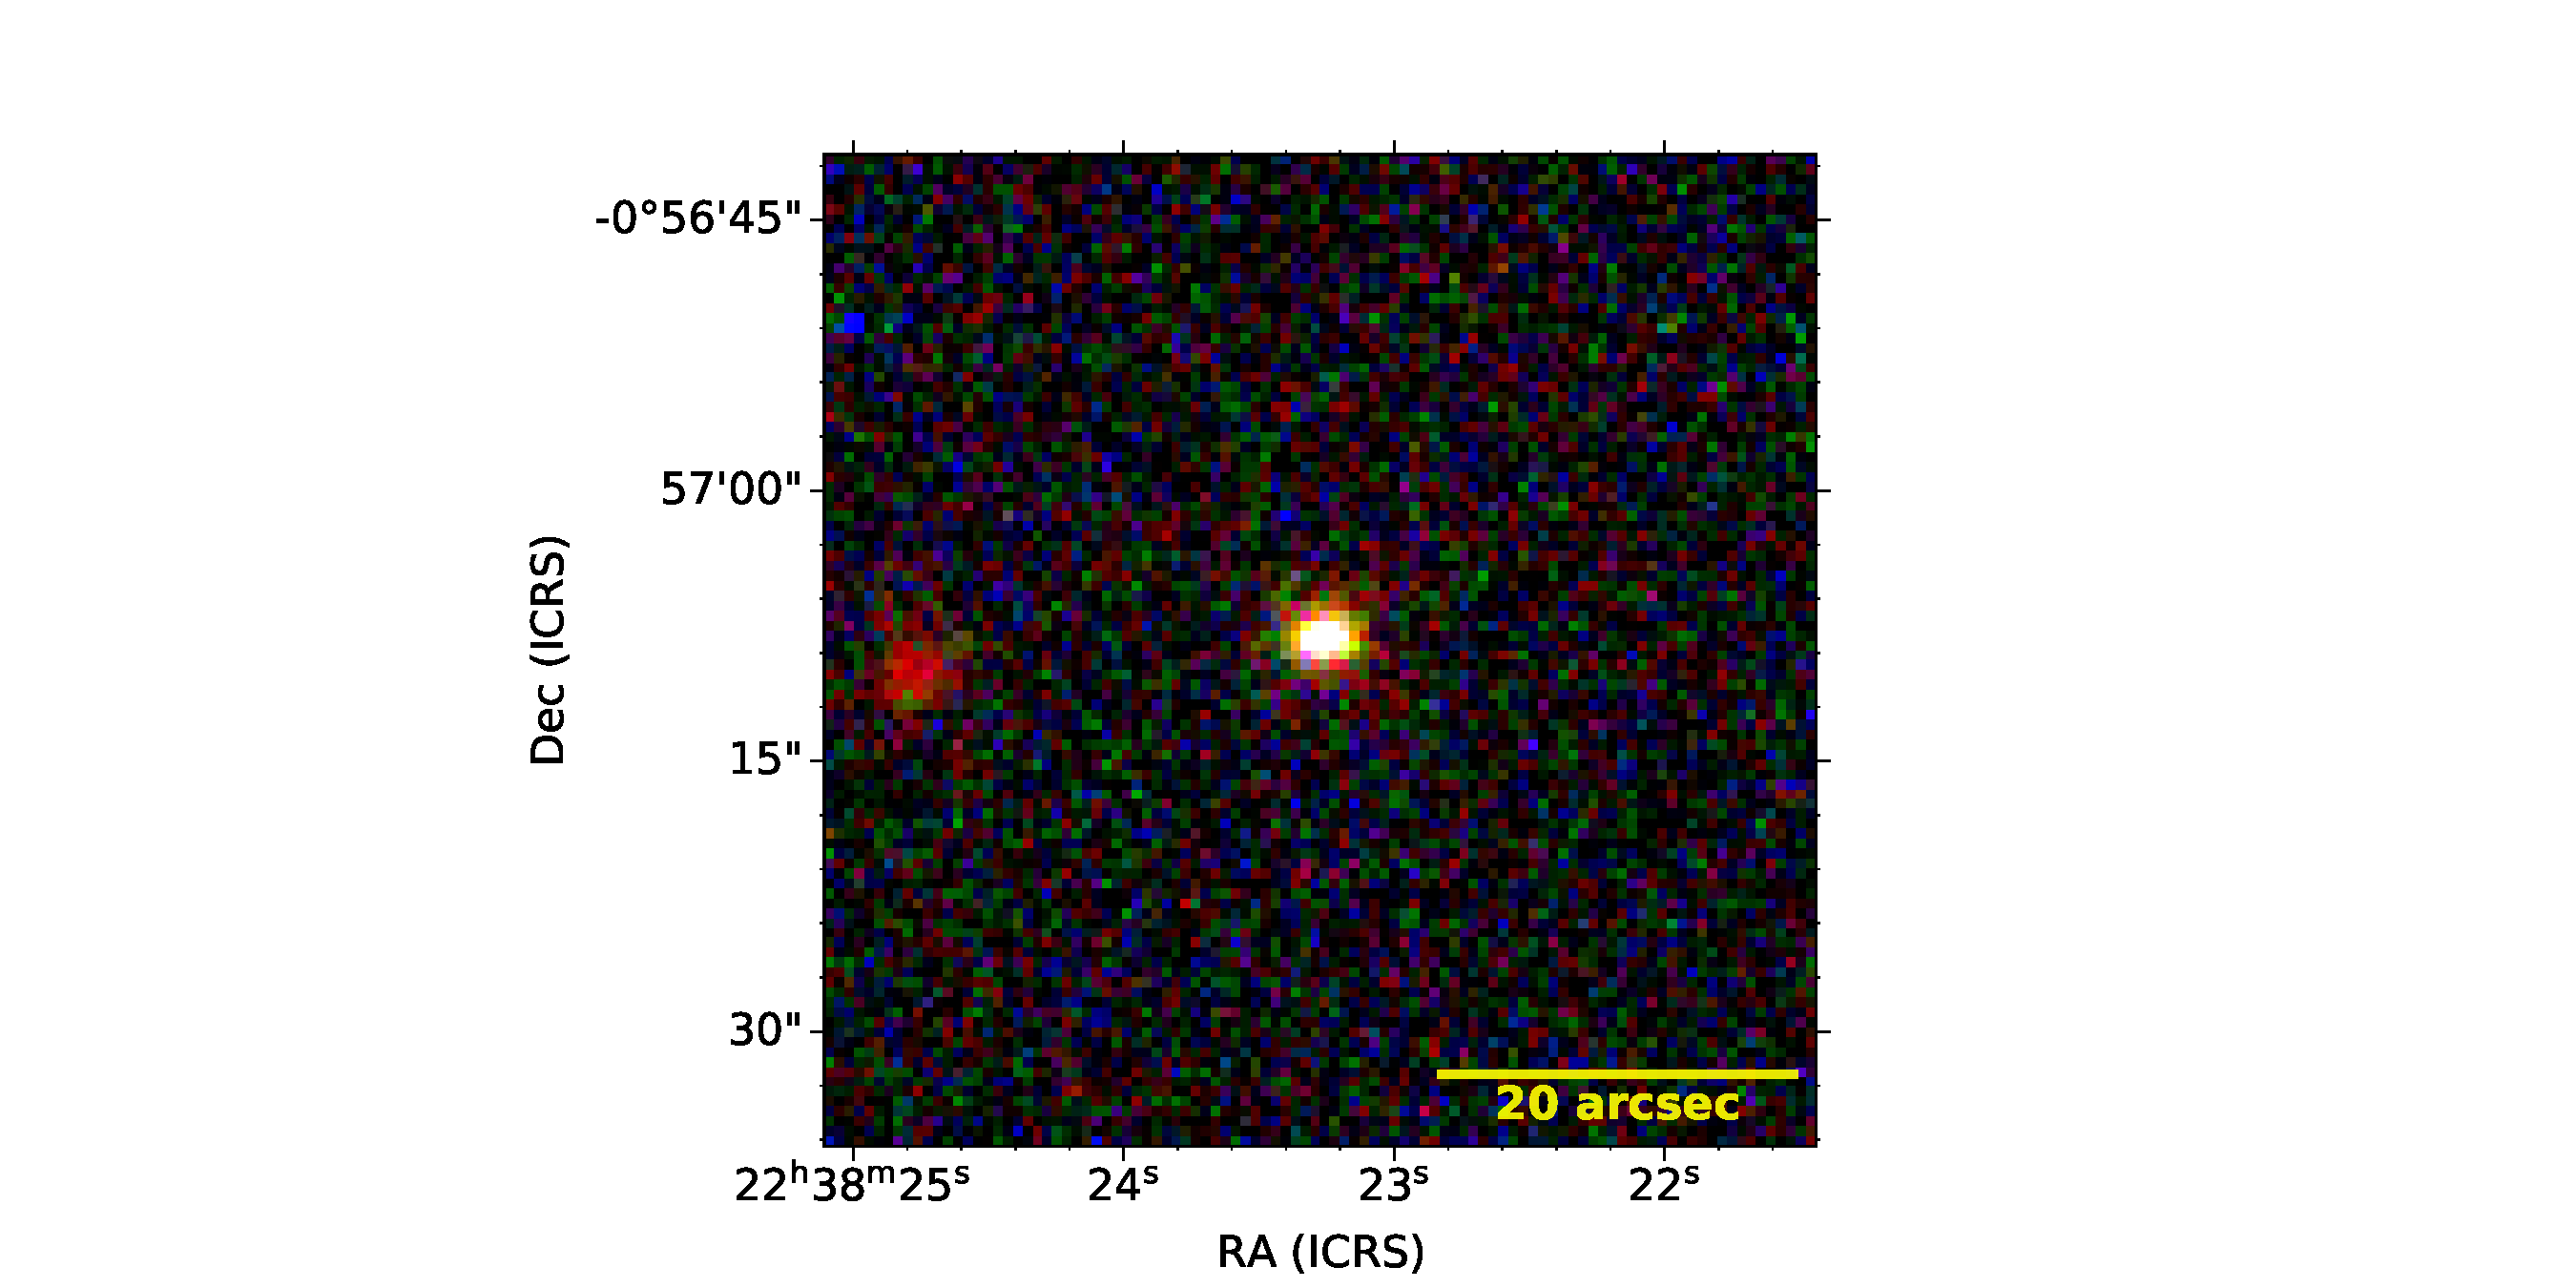
\includegraphics[width=0.4\linewidth, trim=10 0 10 20, clip]{Figs/PHL354_339-0_100_r.pdf} \\
  \end{tabular}
  \caption{Spectra of the known objects select with our algorithm }
  \label{fig:color-diagram}
\end{figure*}

\begin{figure*}
  \setlength\tabcolsep{0pt}
  \setkeys{Gin}{width=0.5\linewidth}
  \begin{tabular}{ll}
    (a) & (b) \\
    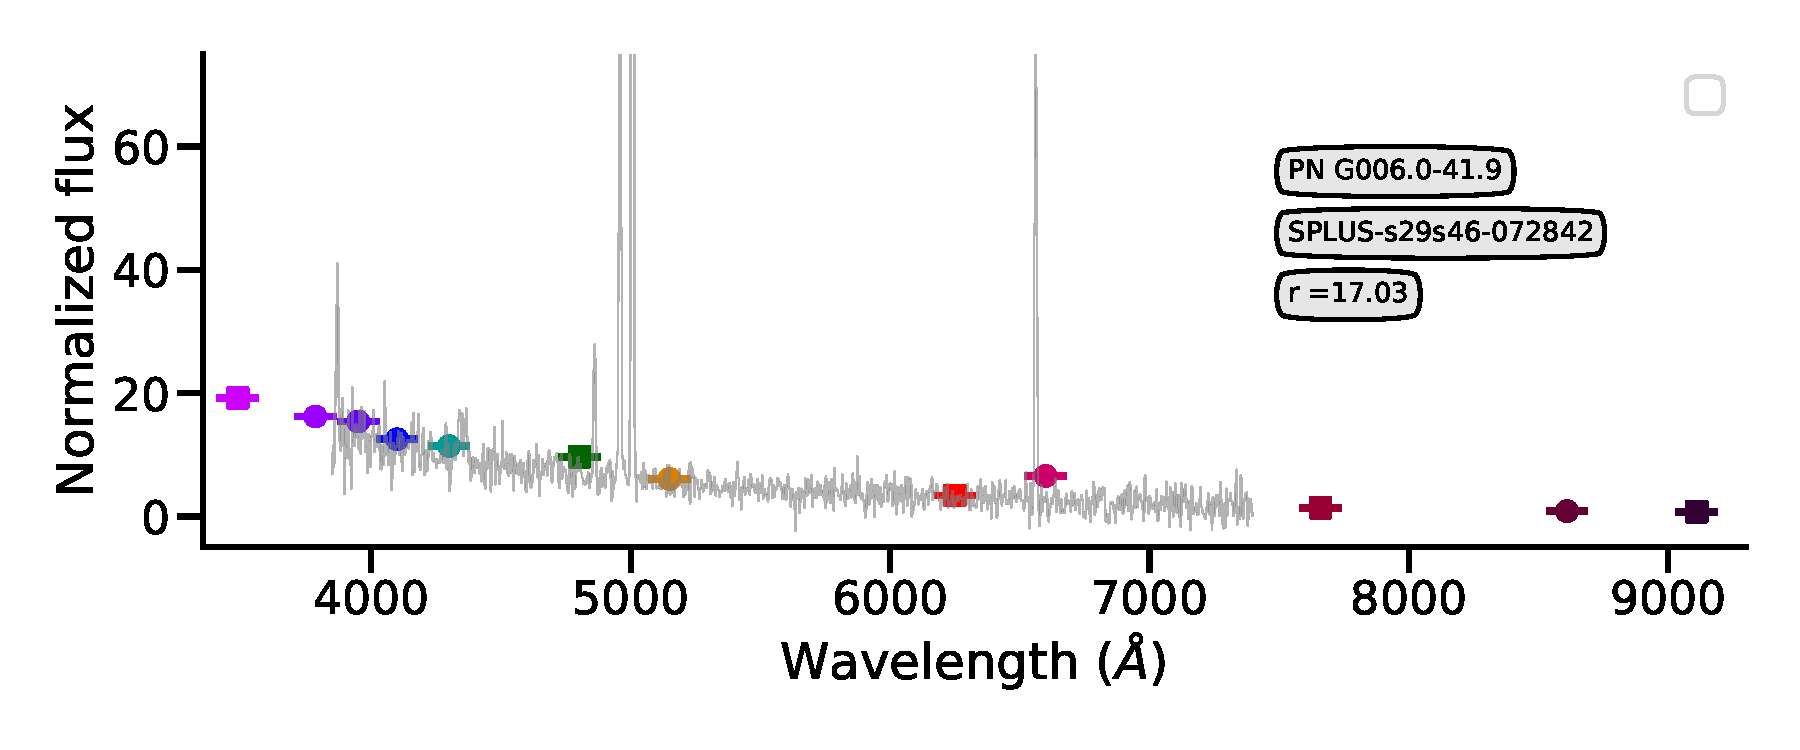
\includegraphics[trim=10 0 5 10, clip]{Figs/StenholmAcker_pn_g006_0-41_9_id176-SPLUS-s29s46-072842.pdf} & 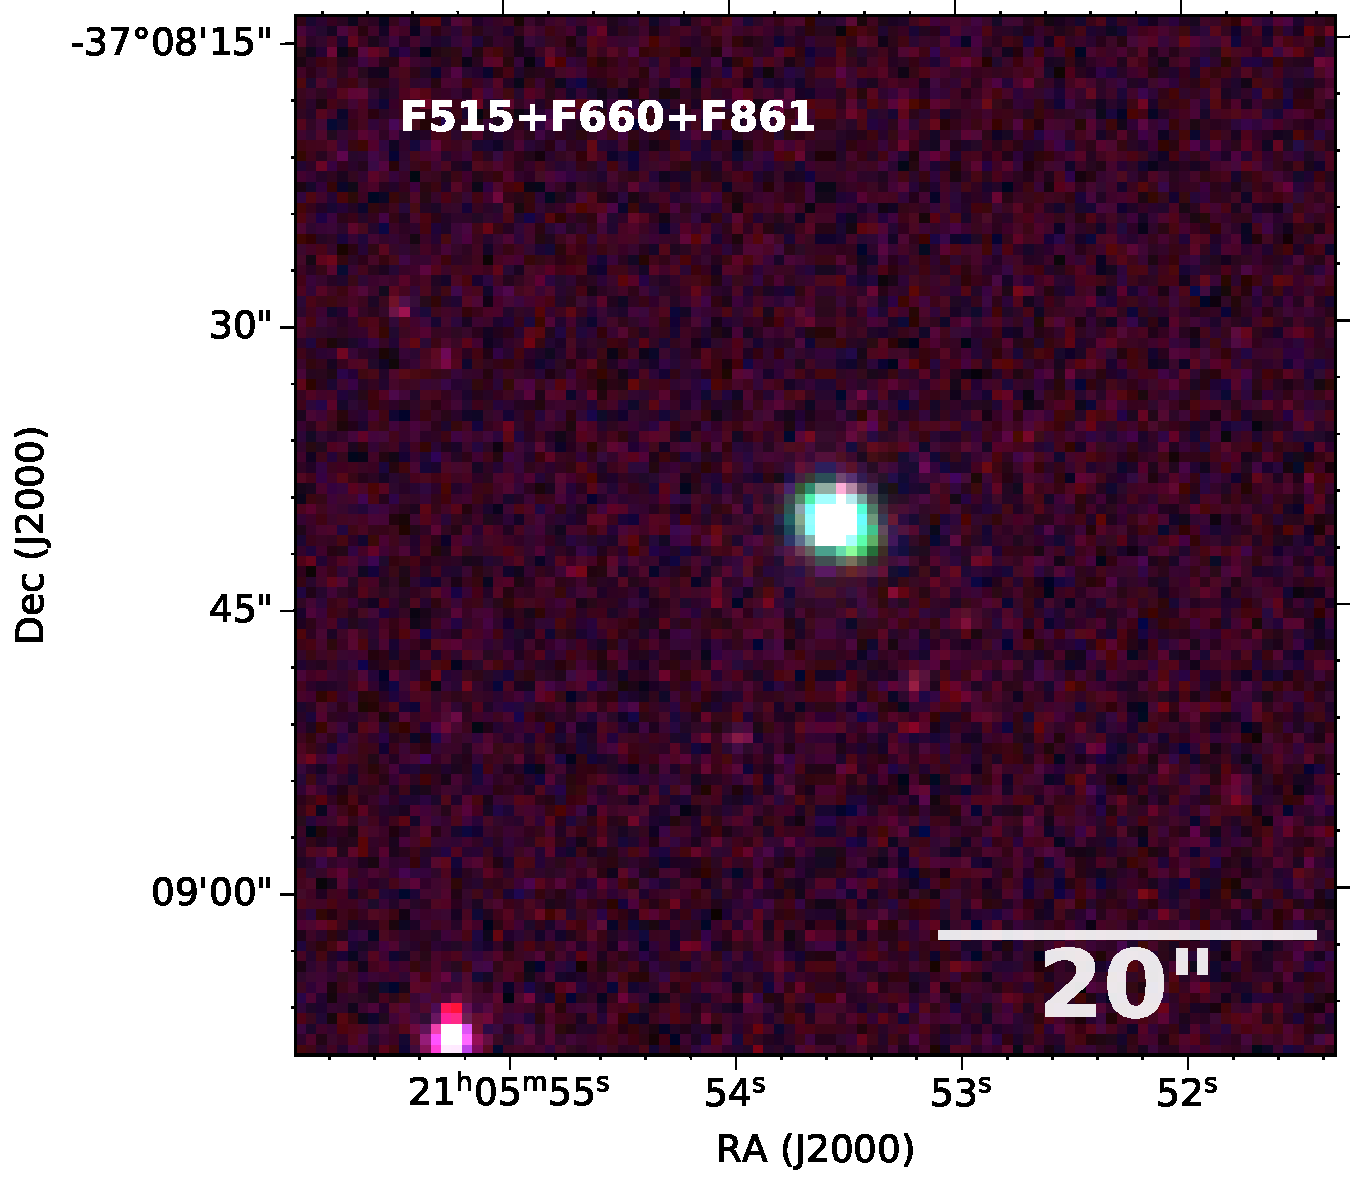
\includegraphics[width=0.2\linewidth, trim=10 0 5 5, clip]{Figs/PNG006_316--37_100_F660-RGB.pdf} \\
     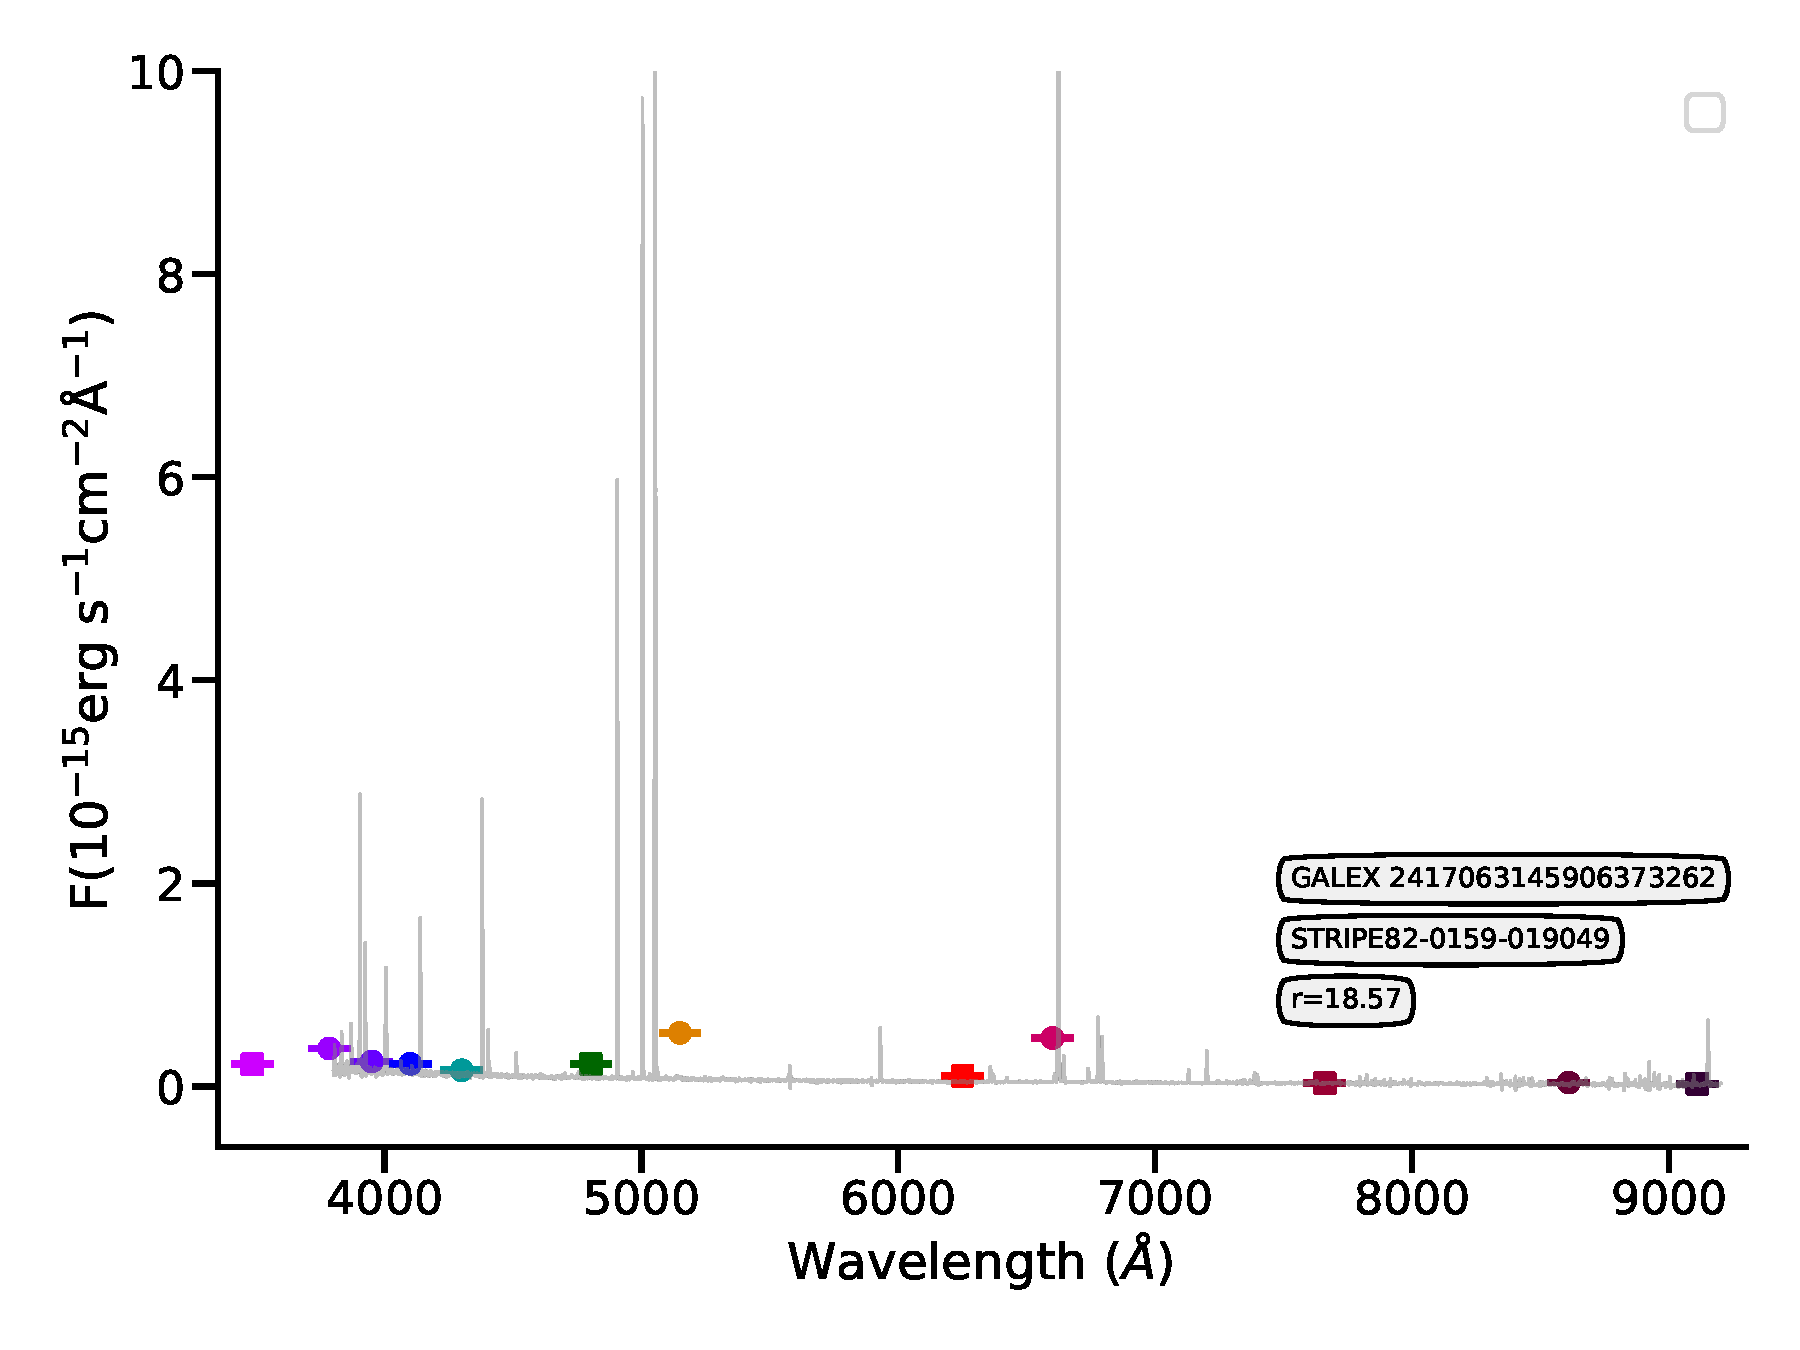
\includegraphics[trim=10 0 5 10, clip]{Figs/spec-0680-52200-0153-STRIPE82-0159-019049.pdf} & 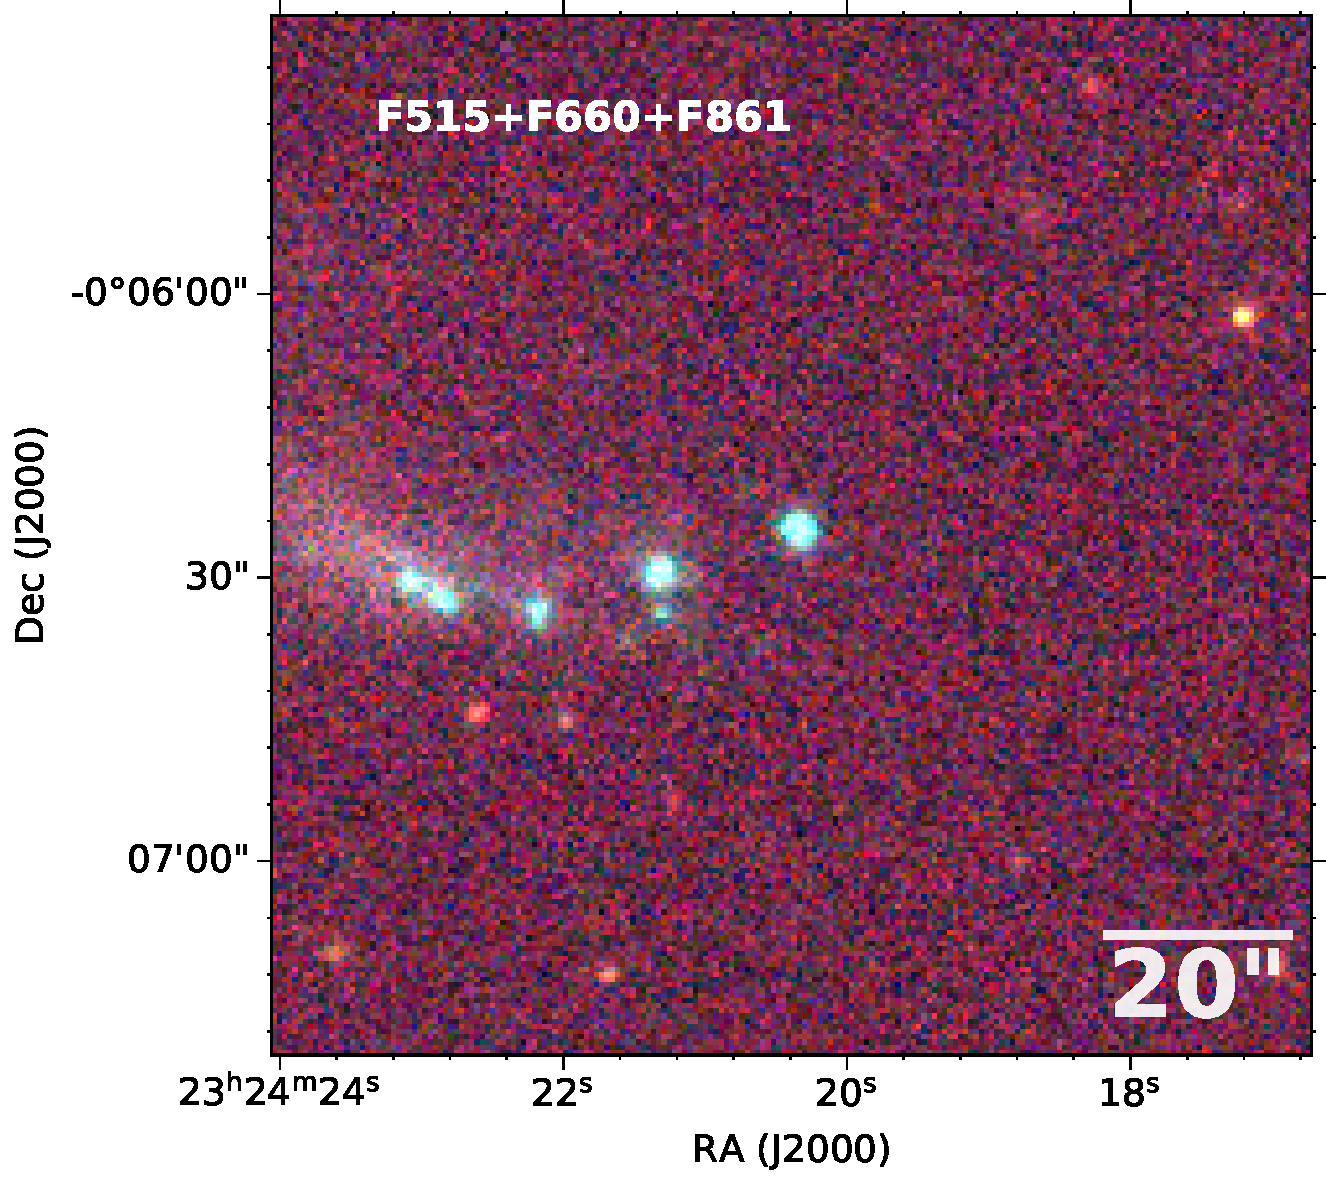
\includegraphics[width=0.2\linewidth, trim=10 0 5 5, clip]{Figs/GALEX24170_351-0_200_F660-RGB.pdf} \\
    (c) & (d) \\
    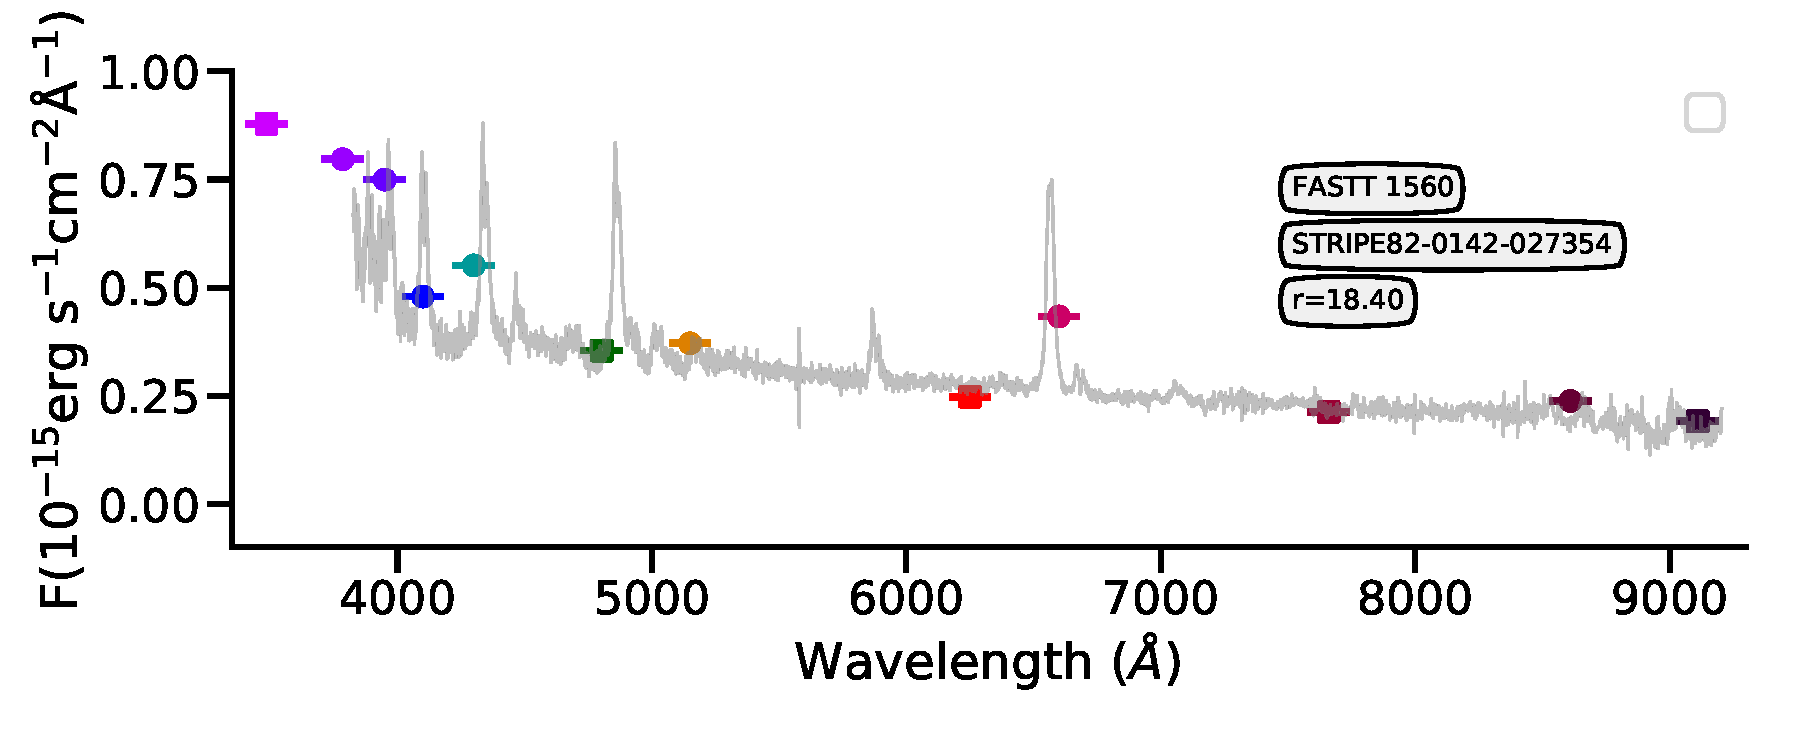
\includegraphics[trim=10 0 5 10, clip]{Figs/spec-0376-52143-0631-STRIPE82-0142-027354.pdf} & 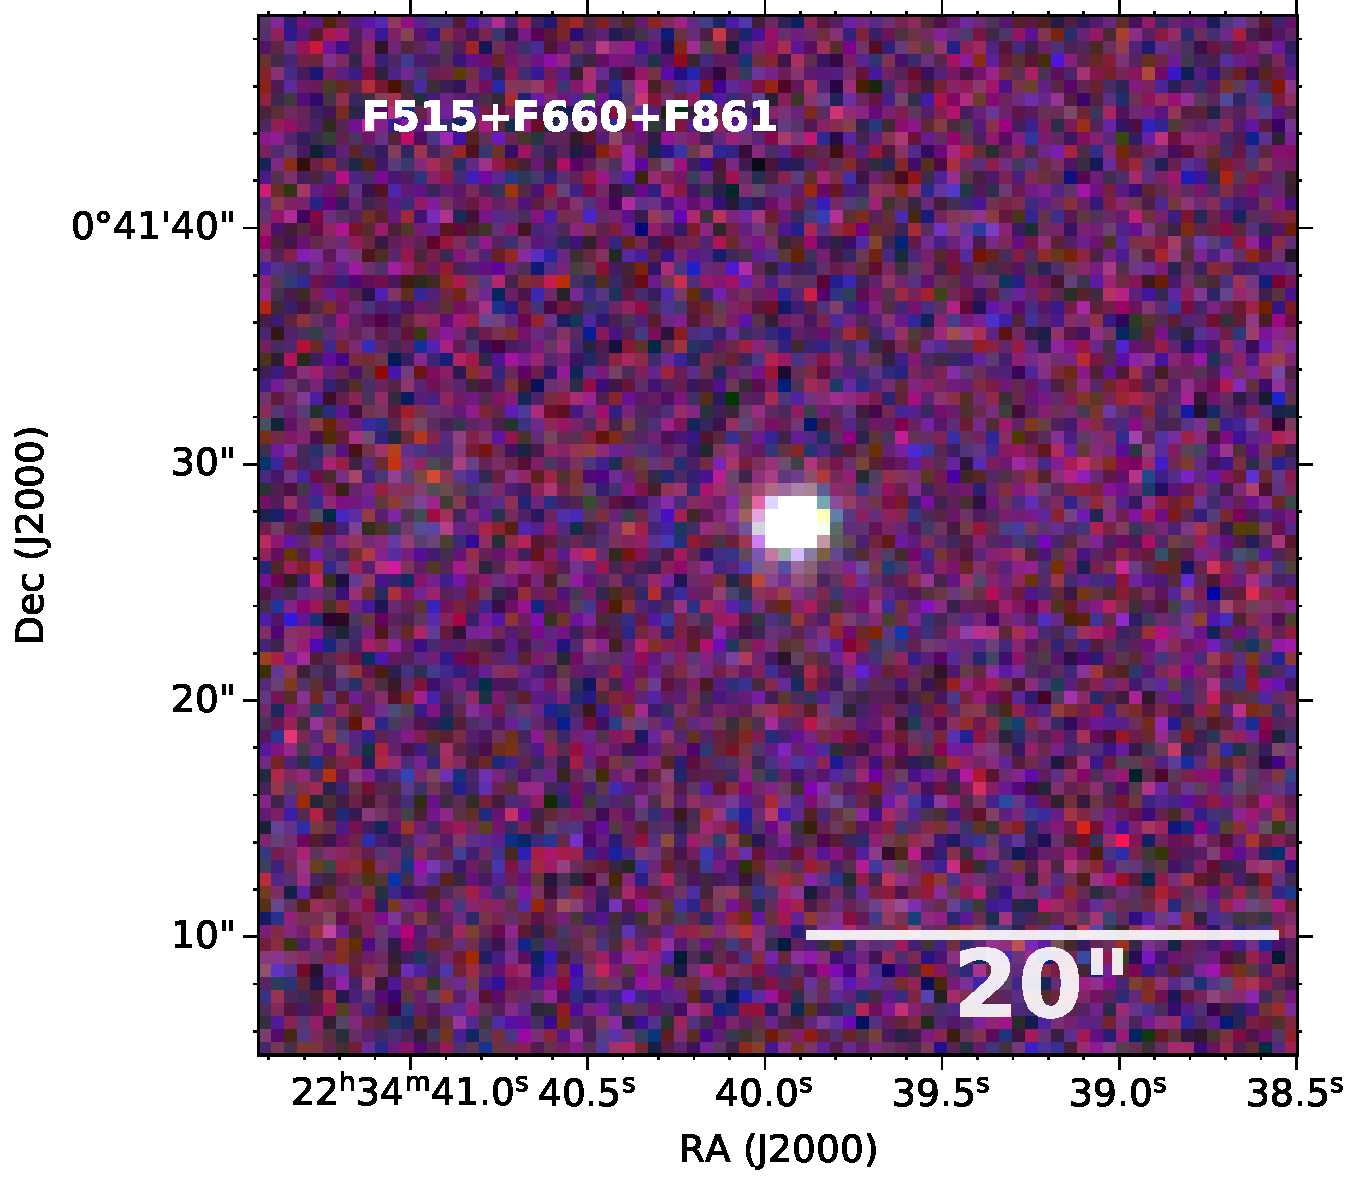
\includegraphics[width=0.2\linewidth, trim=10 0 5 5, clip]{Figs/FASTT1560_338-0_80_F660-RGB.pdf} \\
     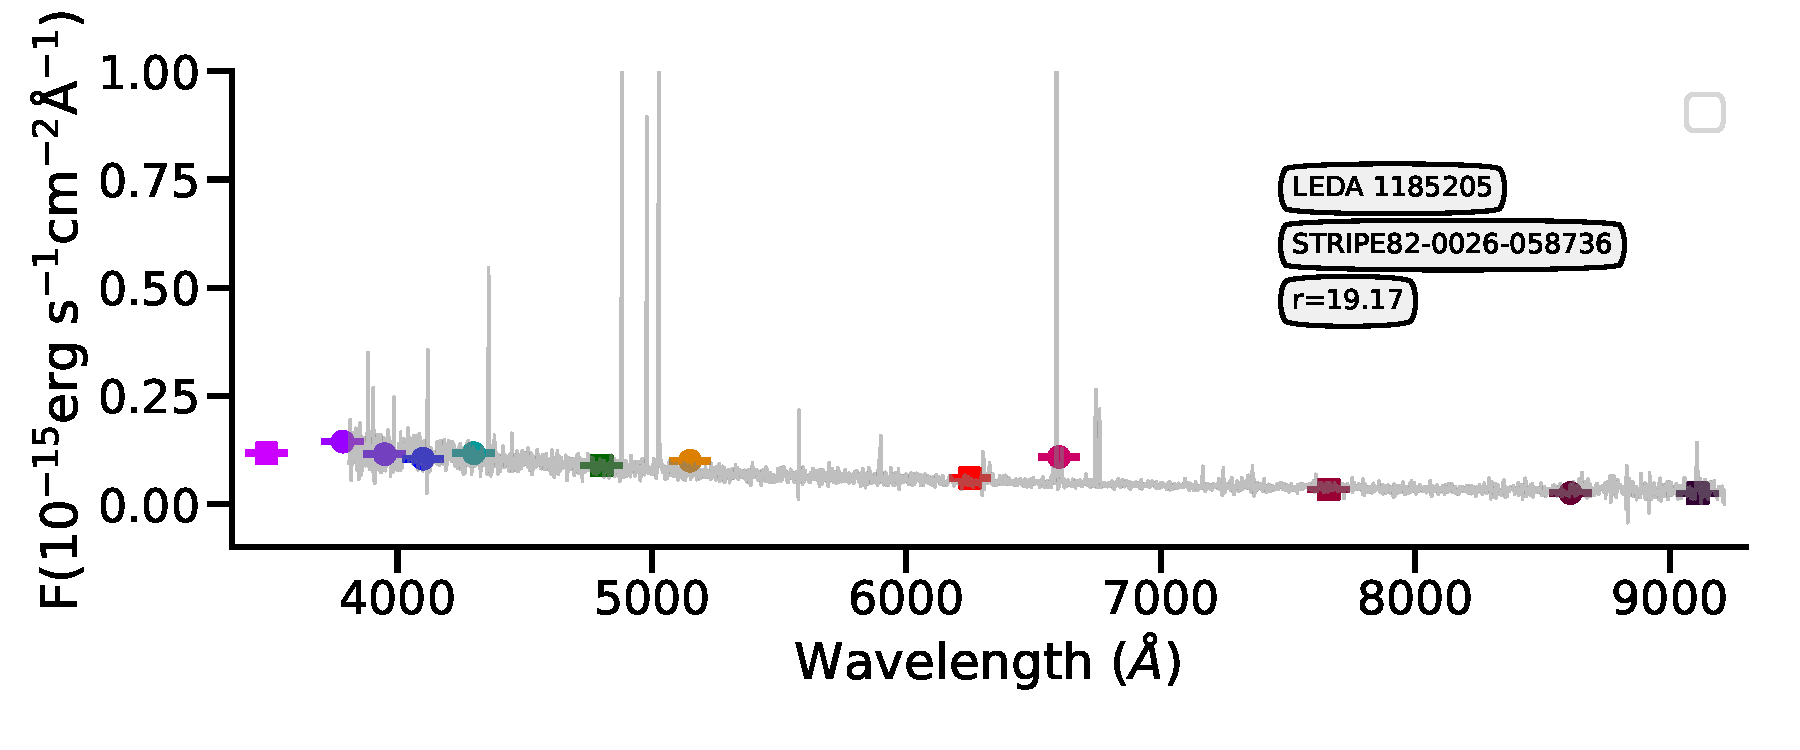
\includegraphics[trim=10 0 5 10, clip]{Figs/spec-0397-51794-0336-STRIPE82-0026-058736.pdf} & 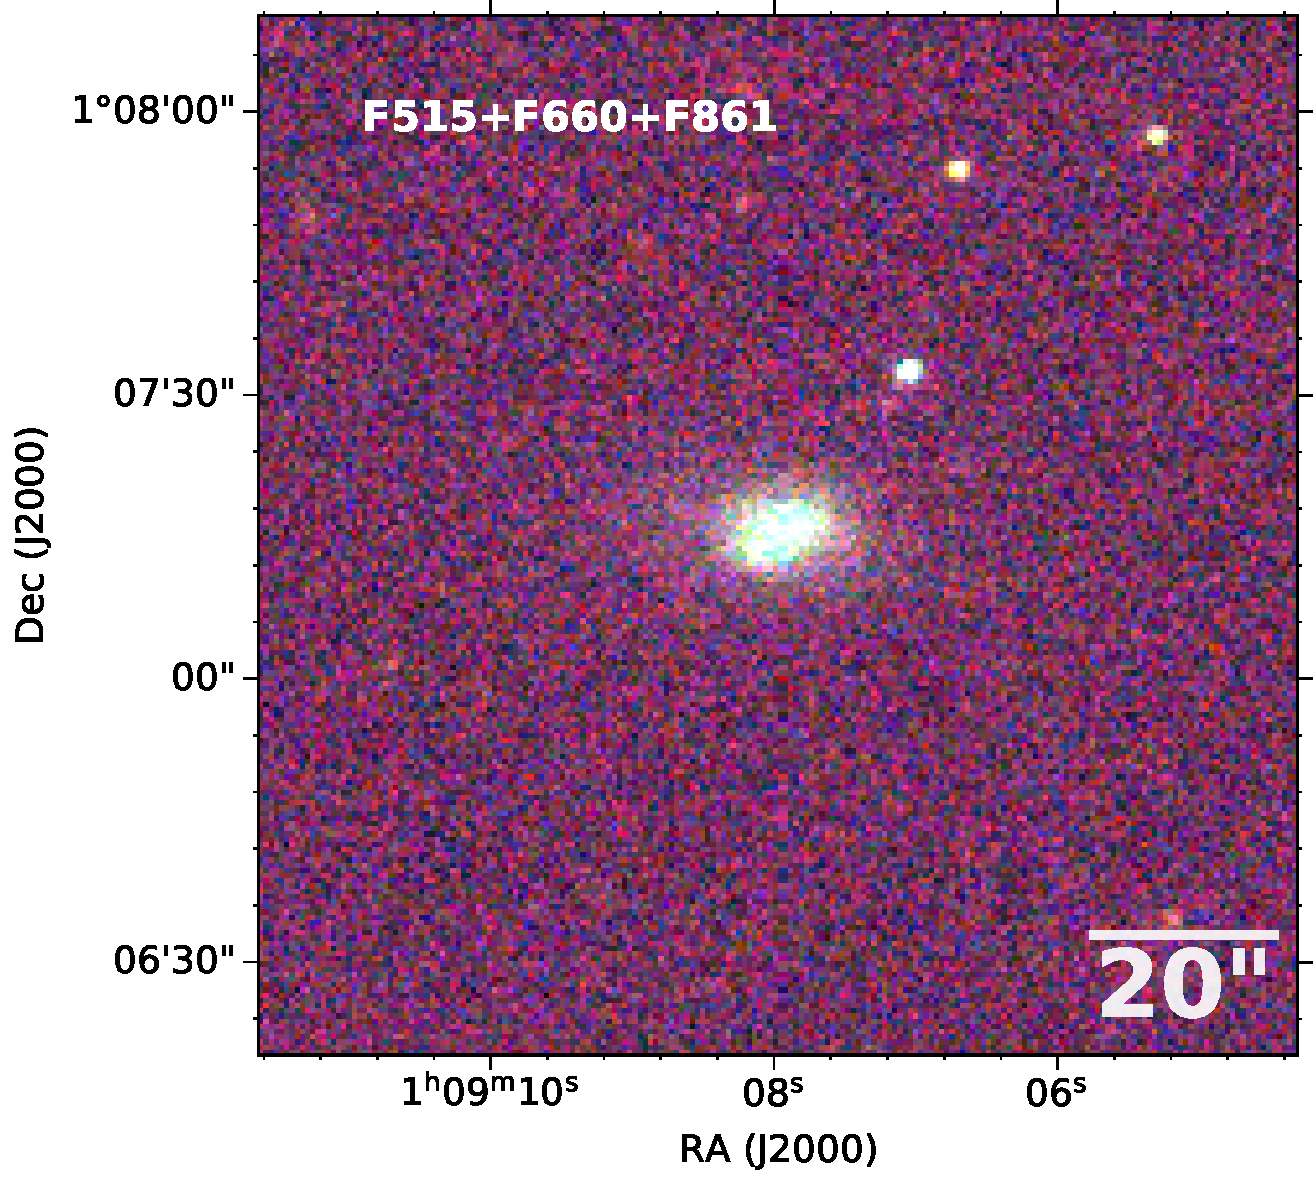
\includegraphics[width=0.2\linewidth, trim=10 0 5 5, clip]{Figs/LEDA1185205_17-1_200_F660-RGB.pdf} \\
     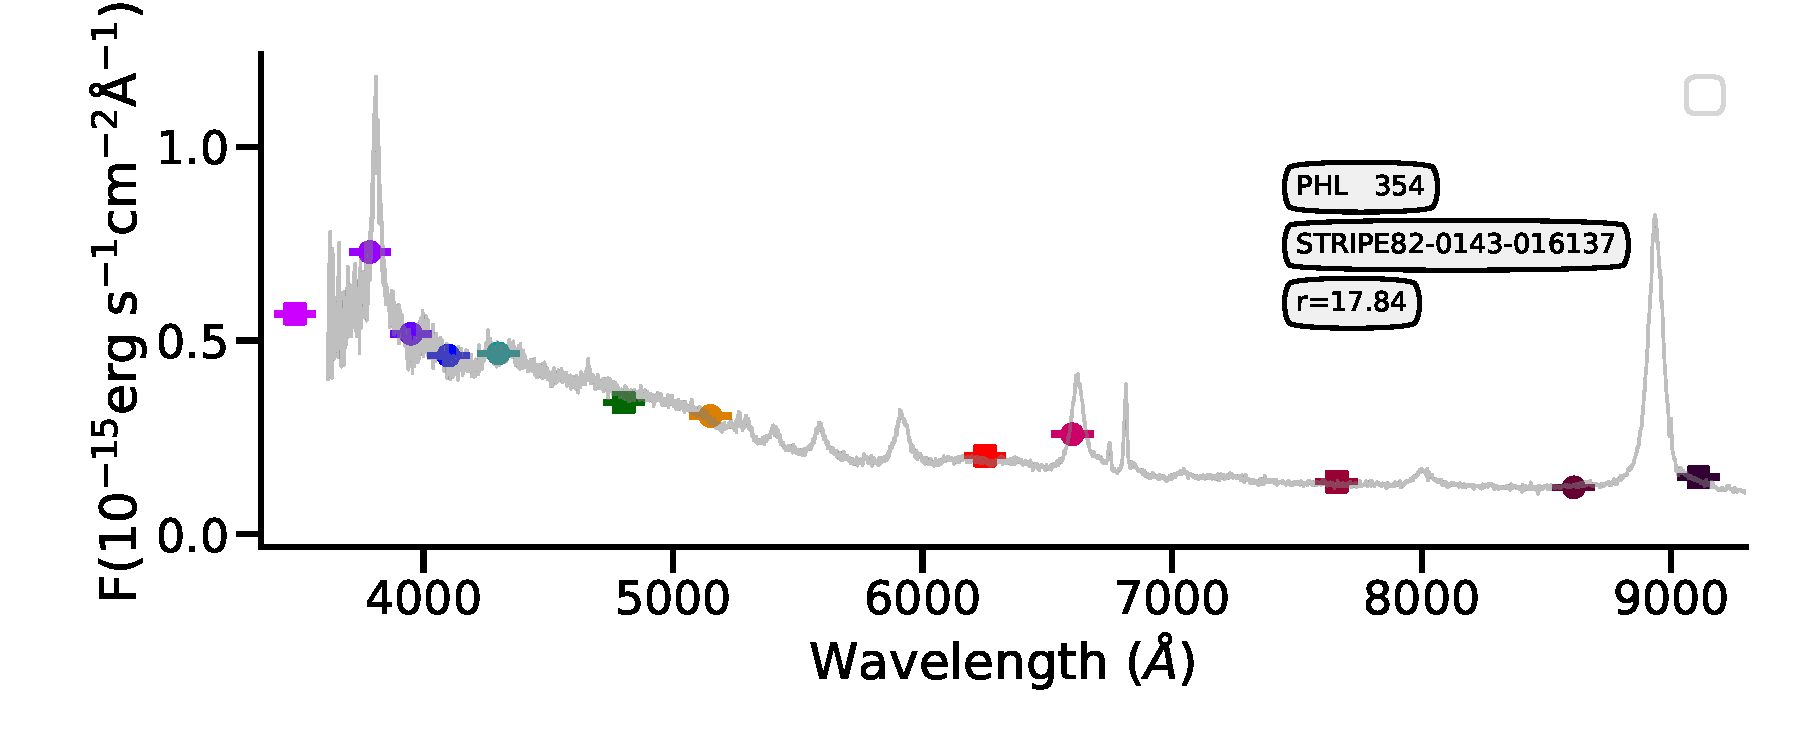
\includegraphics[trim=10 0 5 10, clip]{Figs/spec-9217-57934-0839-STRIPE82-0143-016137.pdf} & 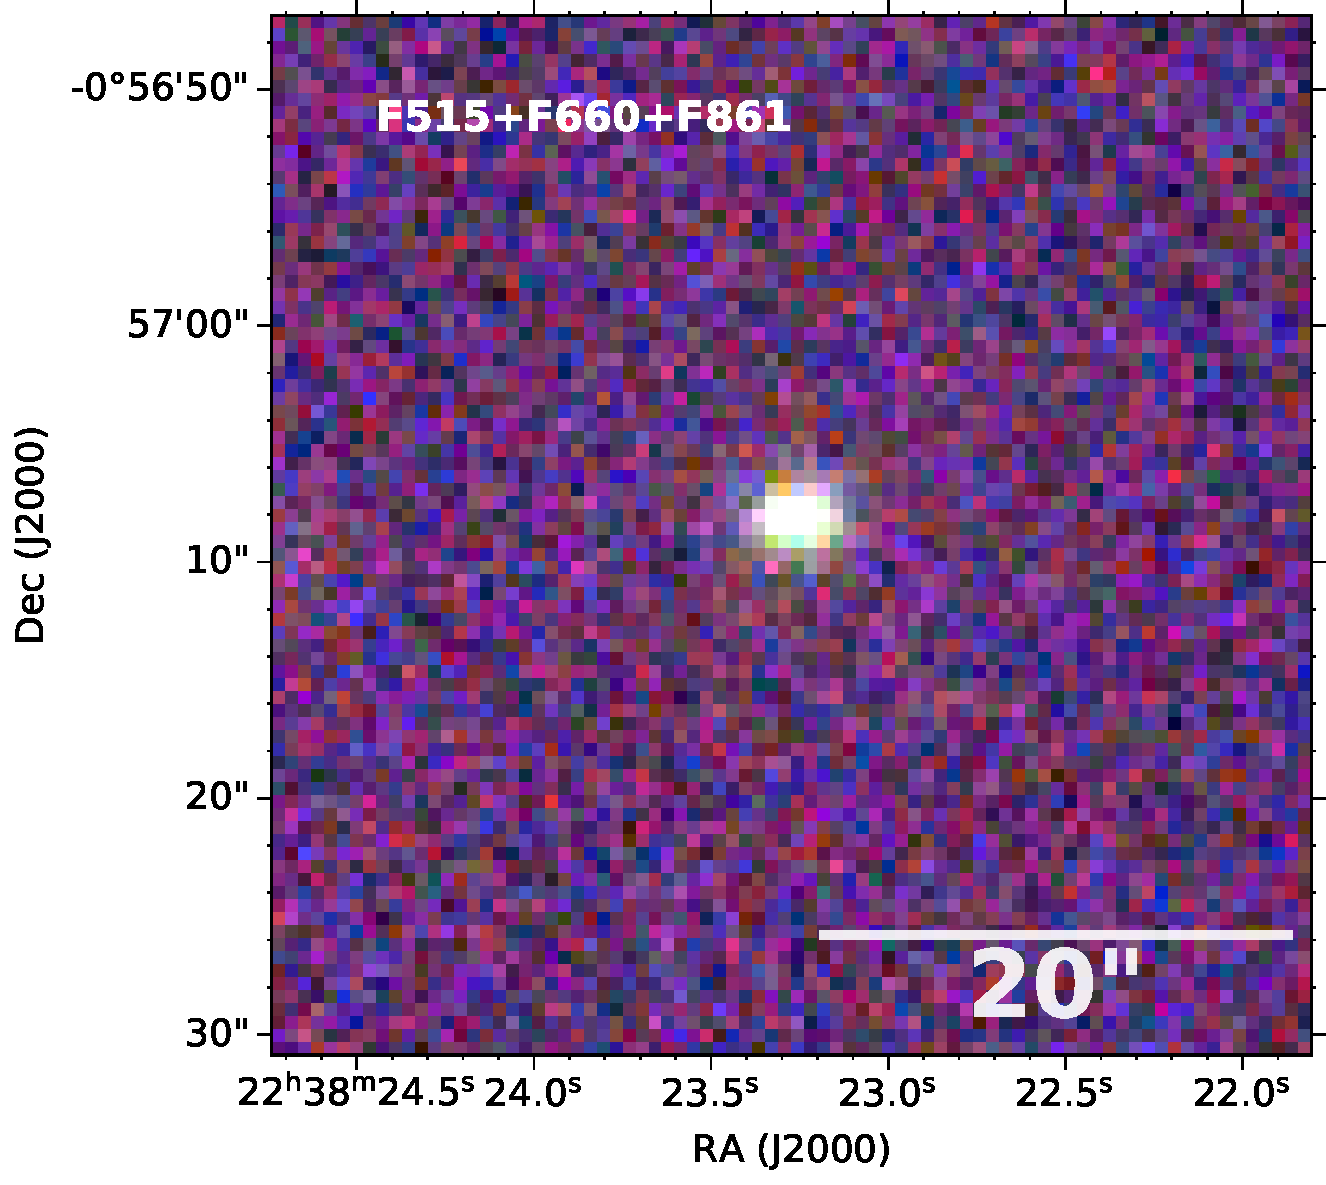
\includegraphics[width=0.2\linewidth, trim=10 0 5 5, clip]{Figs/PHL354_339-0_80_F660-RGB.pdf} \\
  \end{tabular}
  \caption{Spectra of the known objects select with our algorithm }
  \label{fig:color-diagram}
\end{figure*}

\begin{figure*}
  \setlength\tabcolsep{0pt}
  \setkeys{Gin}{width=0.5\linewidth}
  \begin{tabular}{ll}
    (a) & (b) \\
    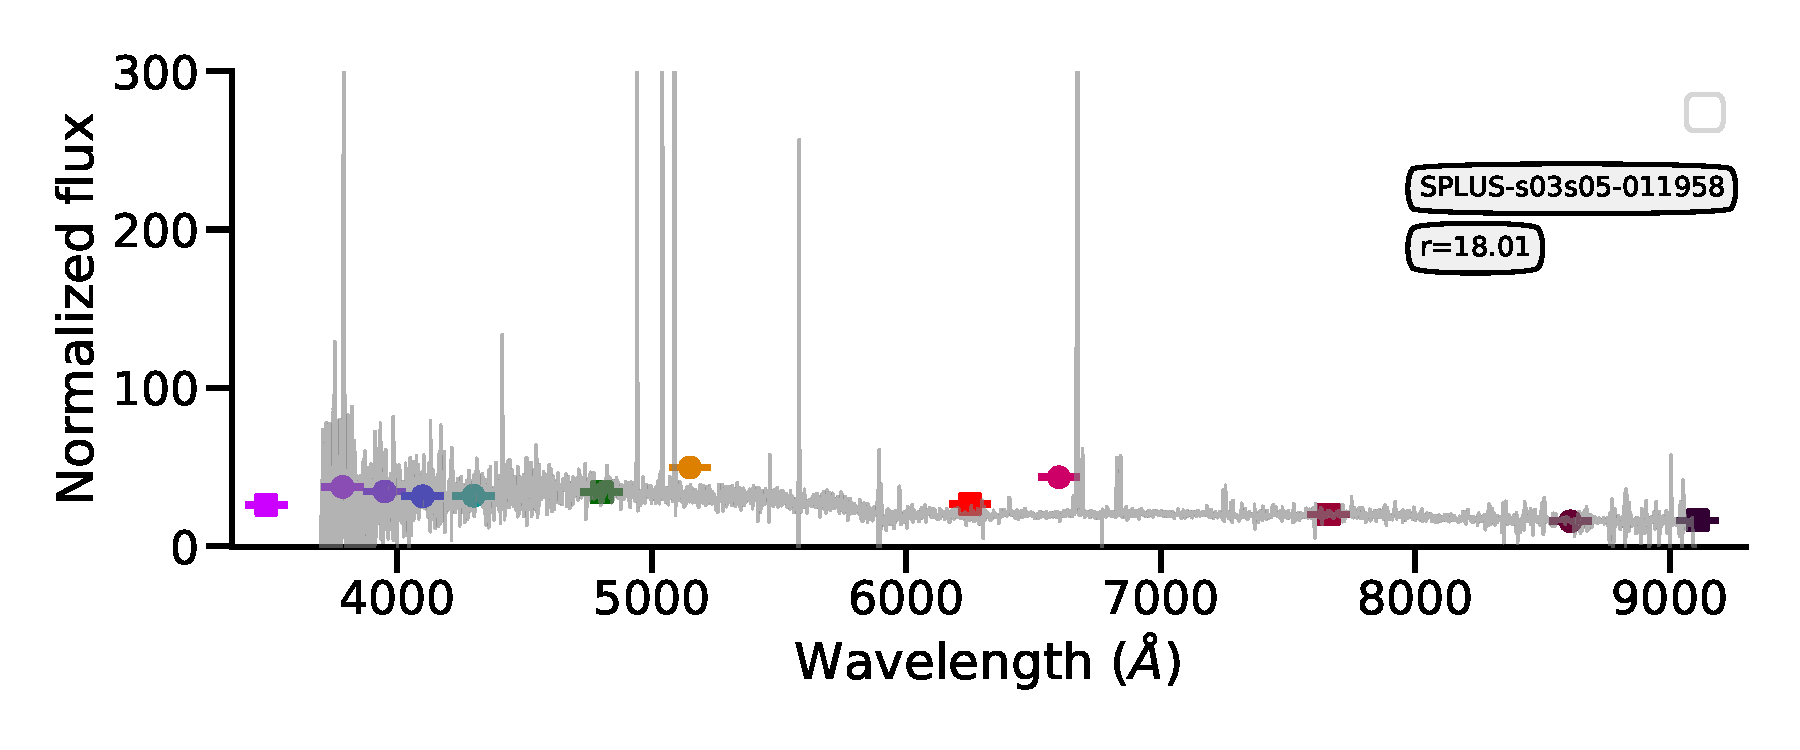
\includegraphics[trim=10 0 10 20, clip]{Figs/spec-57313-EG220318S020919M01_sp10-173-SPLUS-s03s05-011958.pdf} & 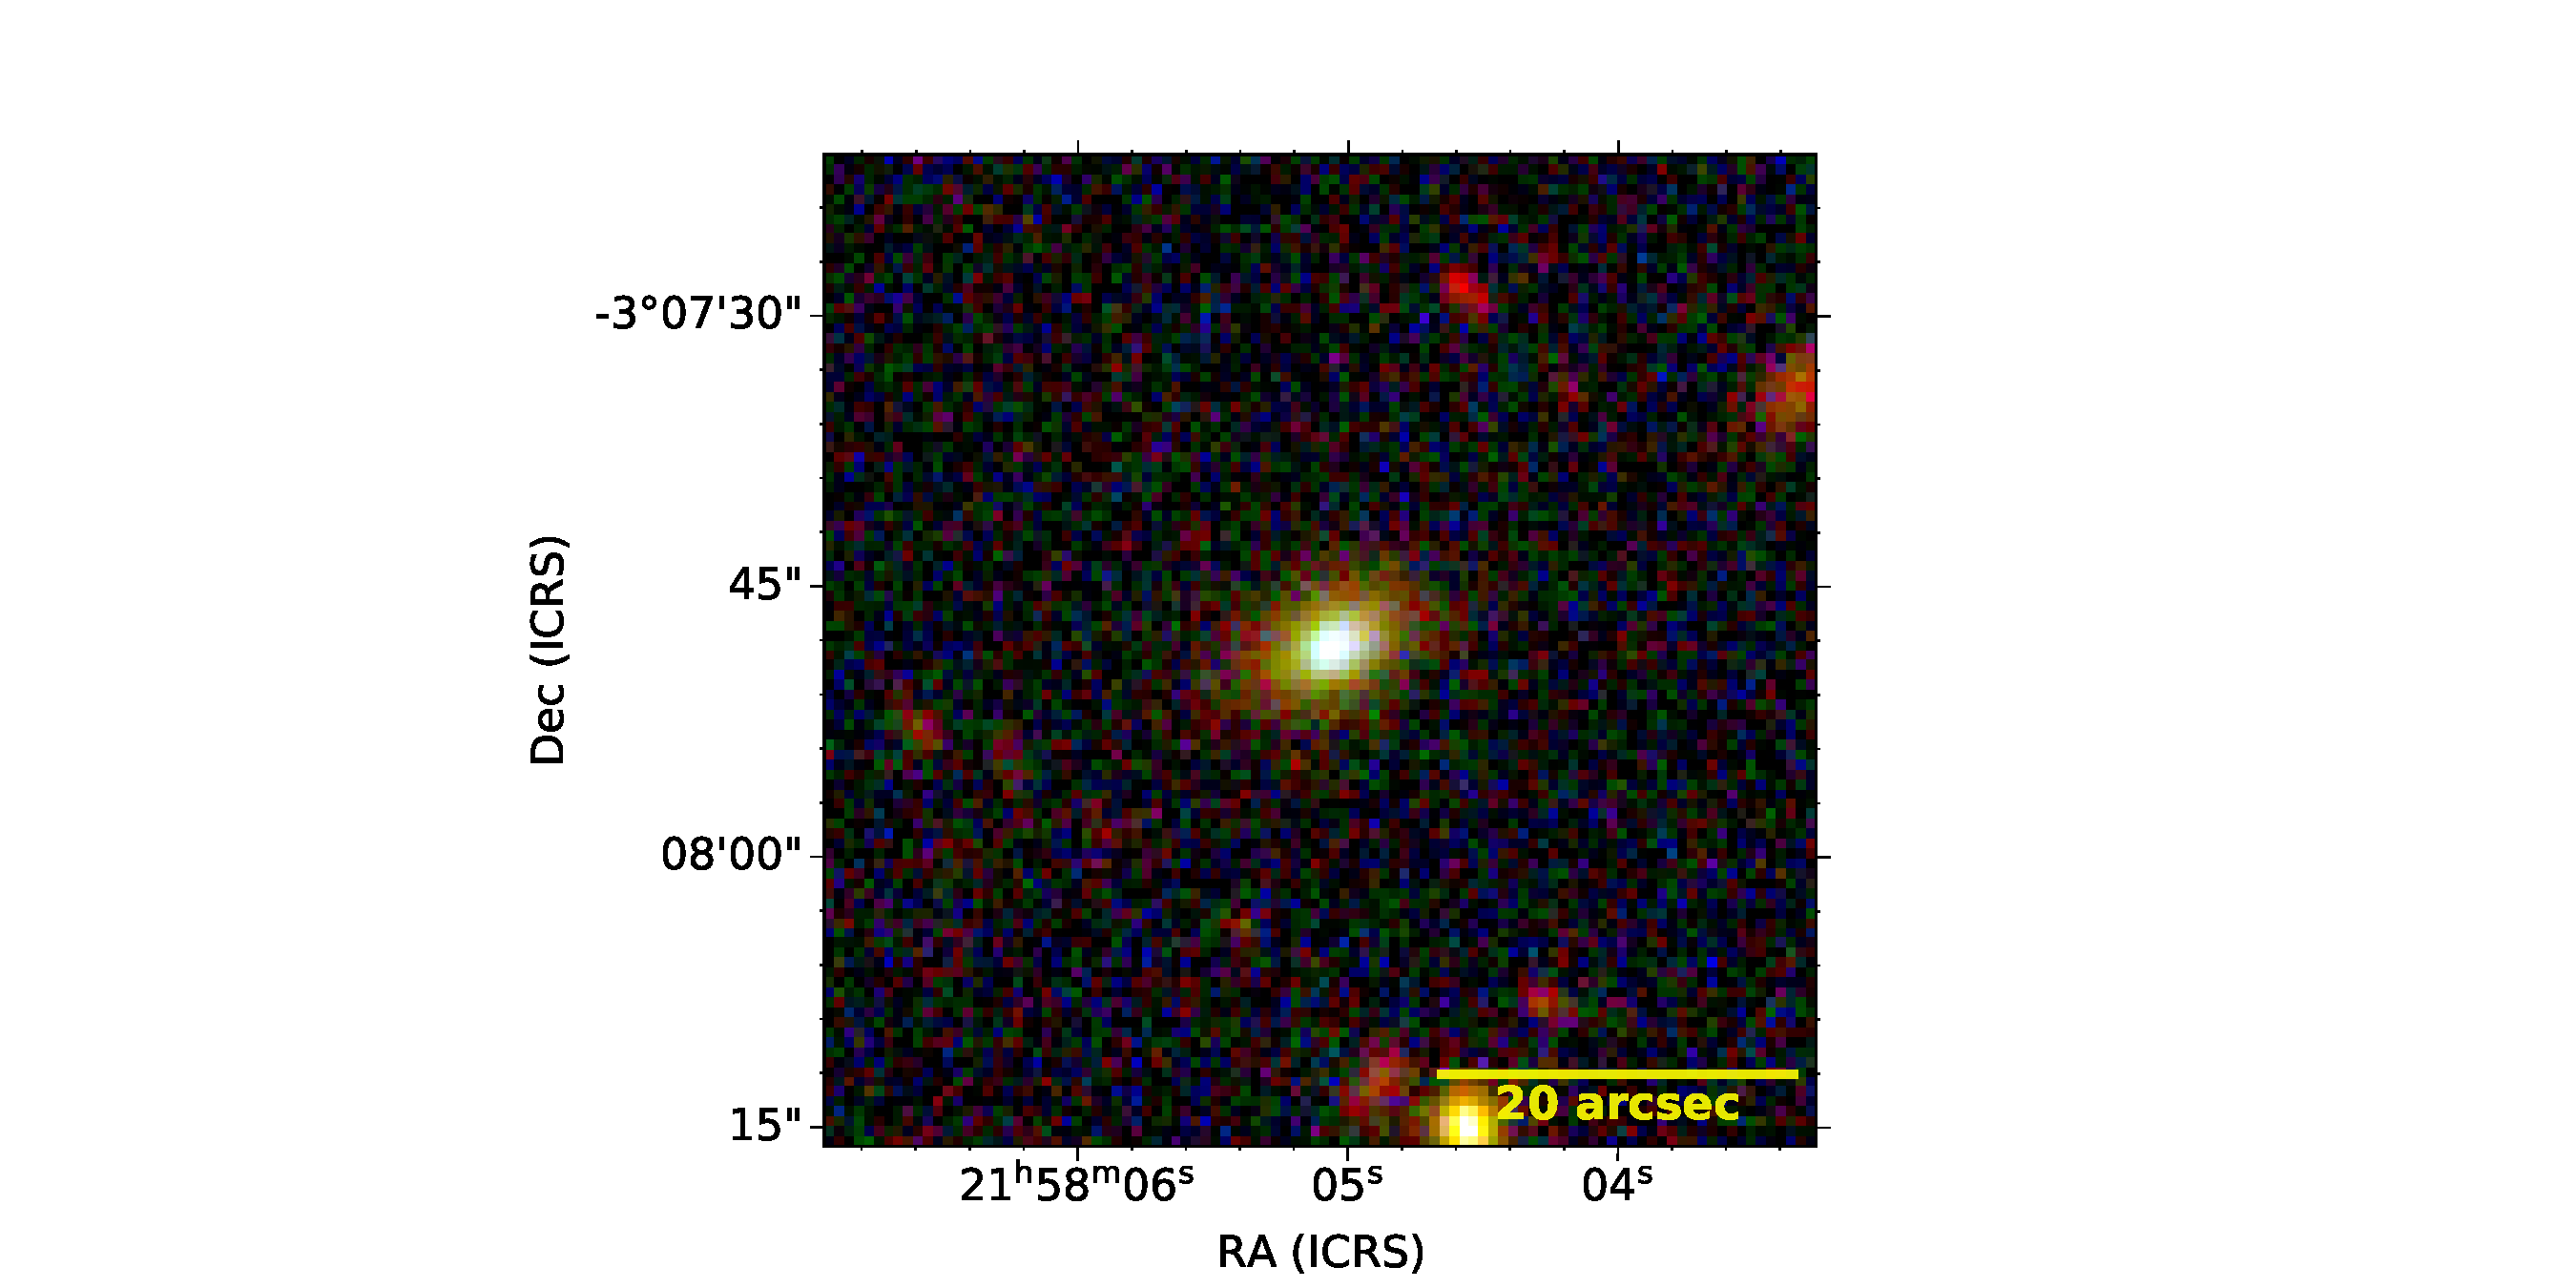
\includegraphics[width=0.4\linewidth, trim=10 0 10 20, clip]{Figs/SPLUS-s03s05-011958_329-3_100_r.pdf} \\
     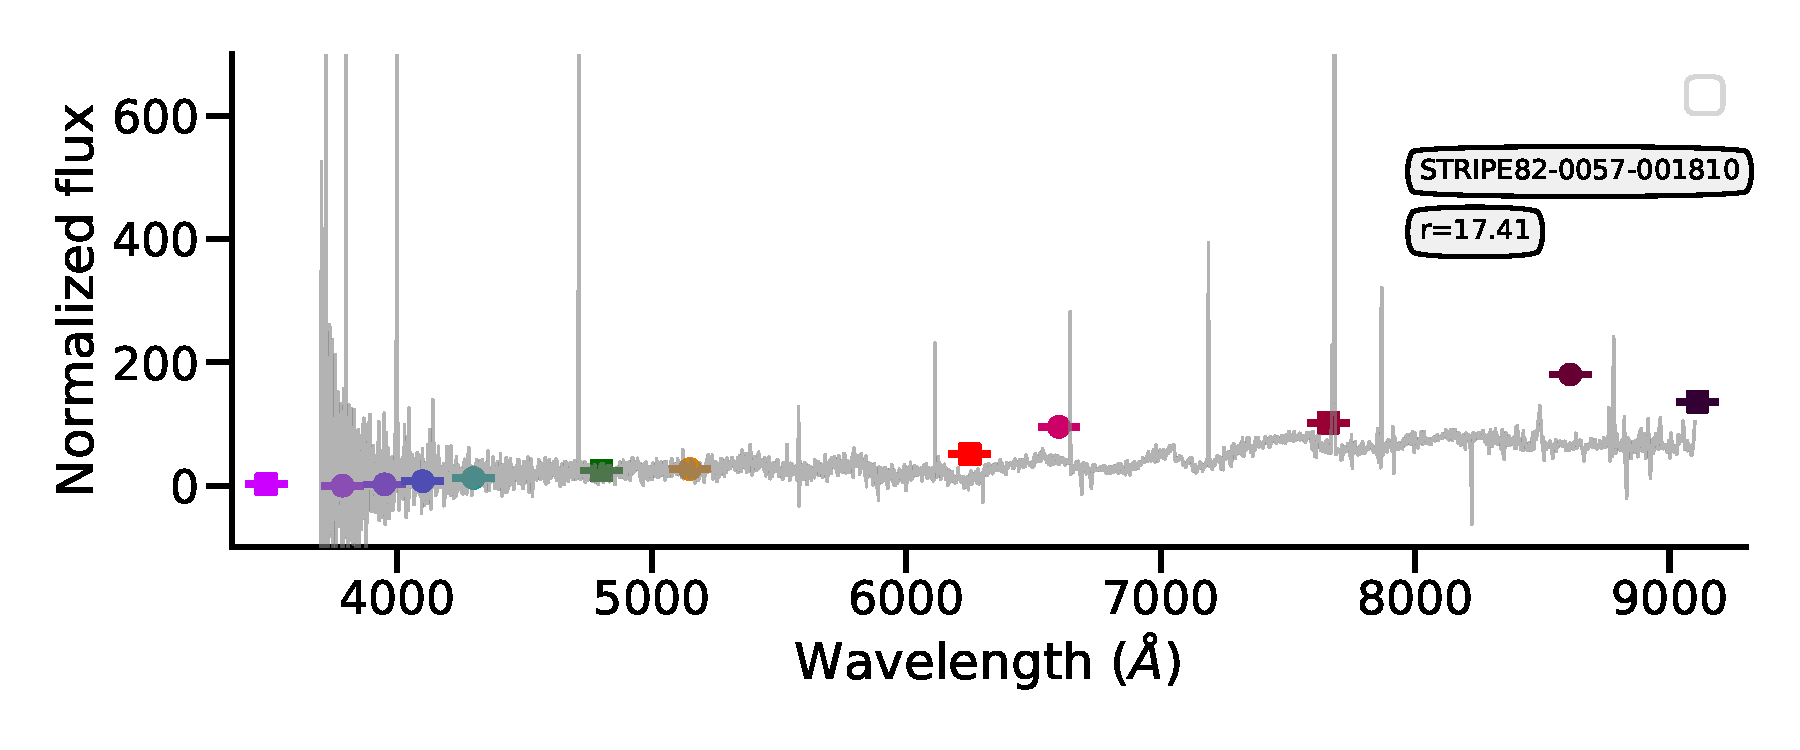
\includegraphics[trim=10 0 10 20, clip]{Figs/spec-55893-F9304_sp15-198-STRIPE82-0057-001810.pdf} & 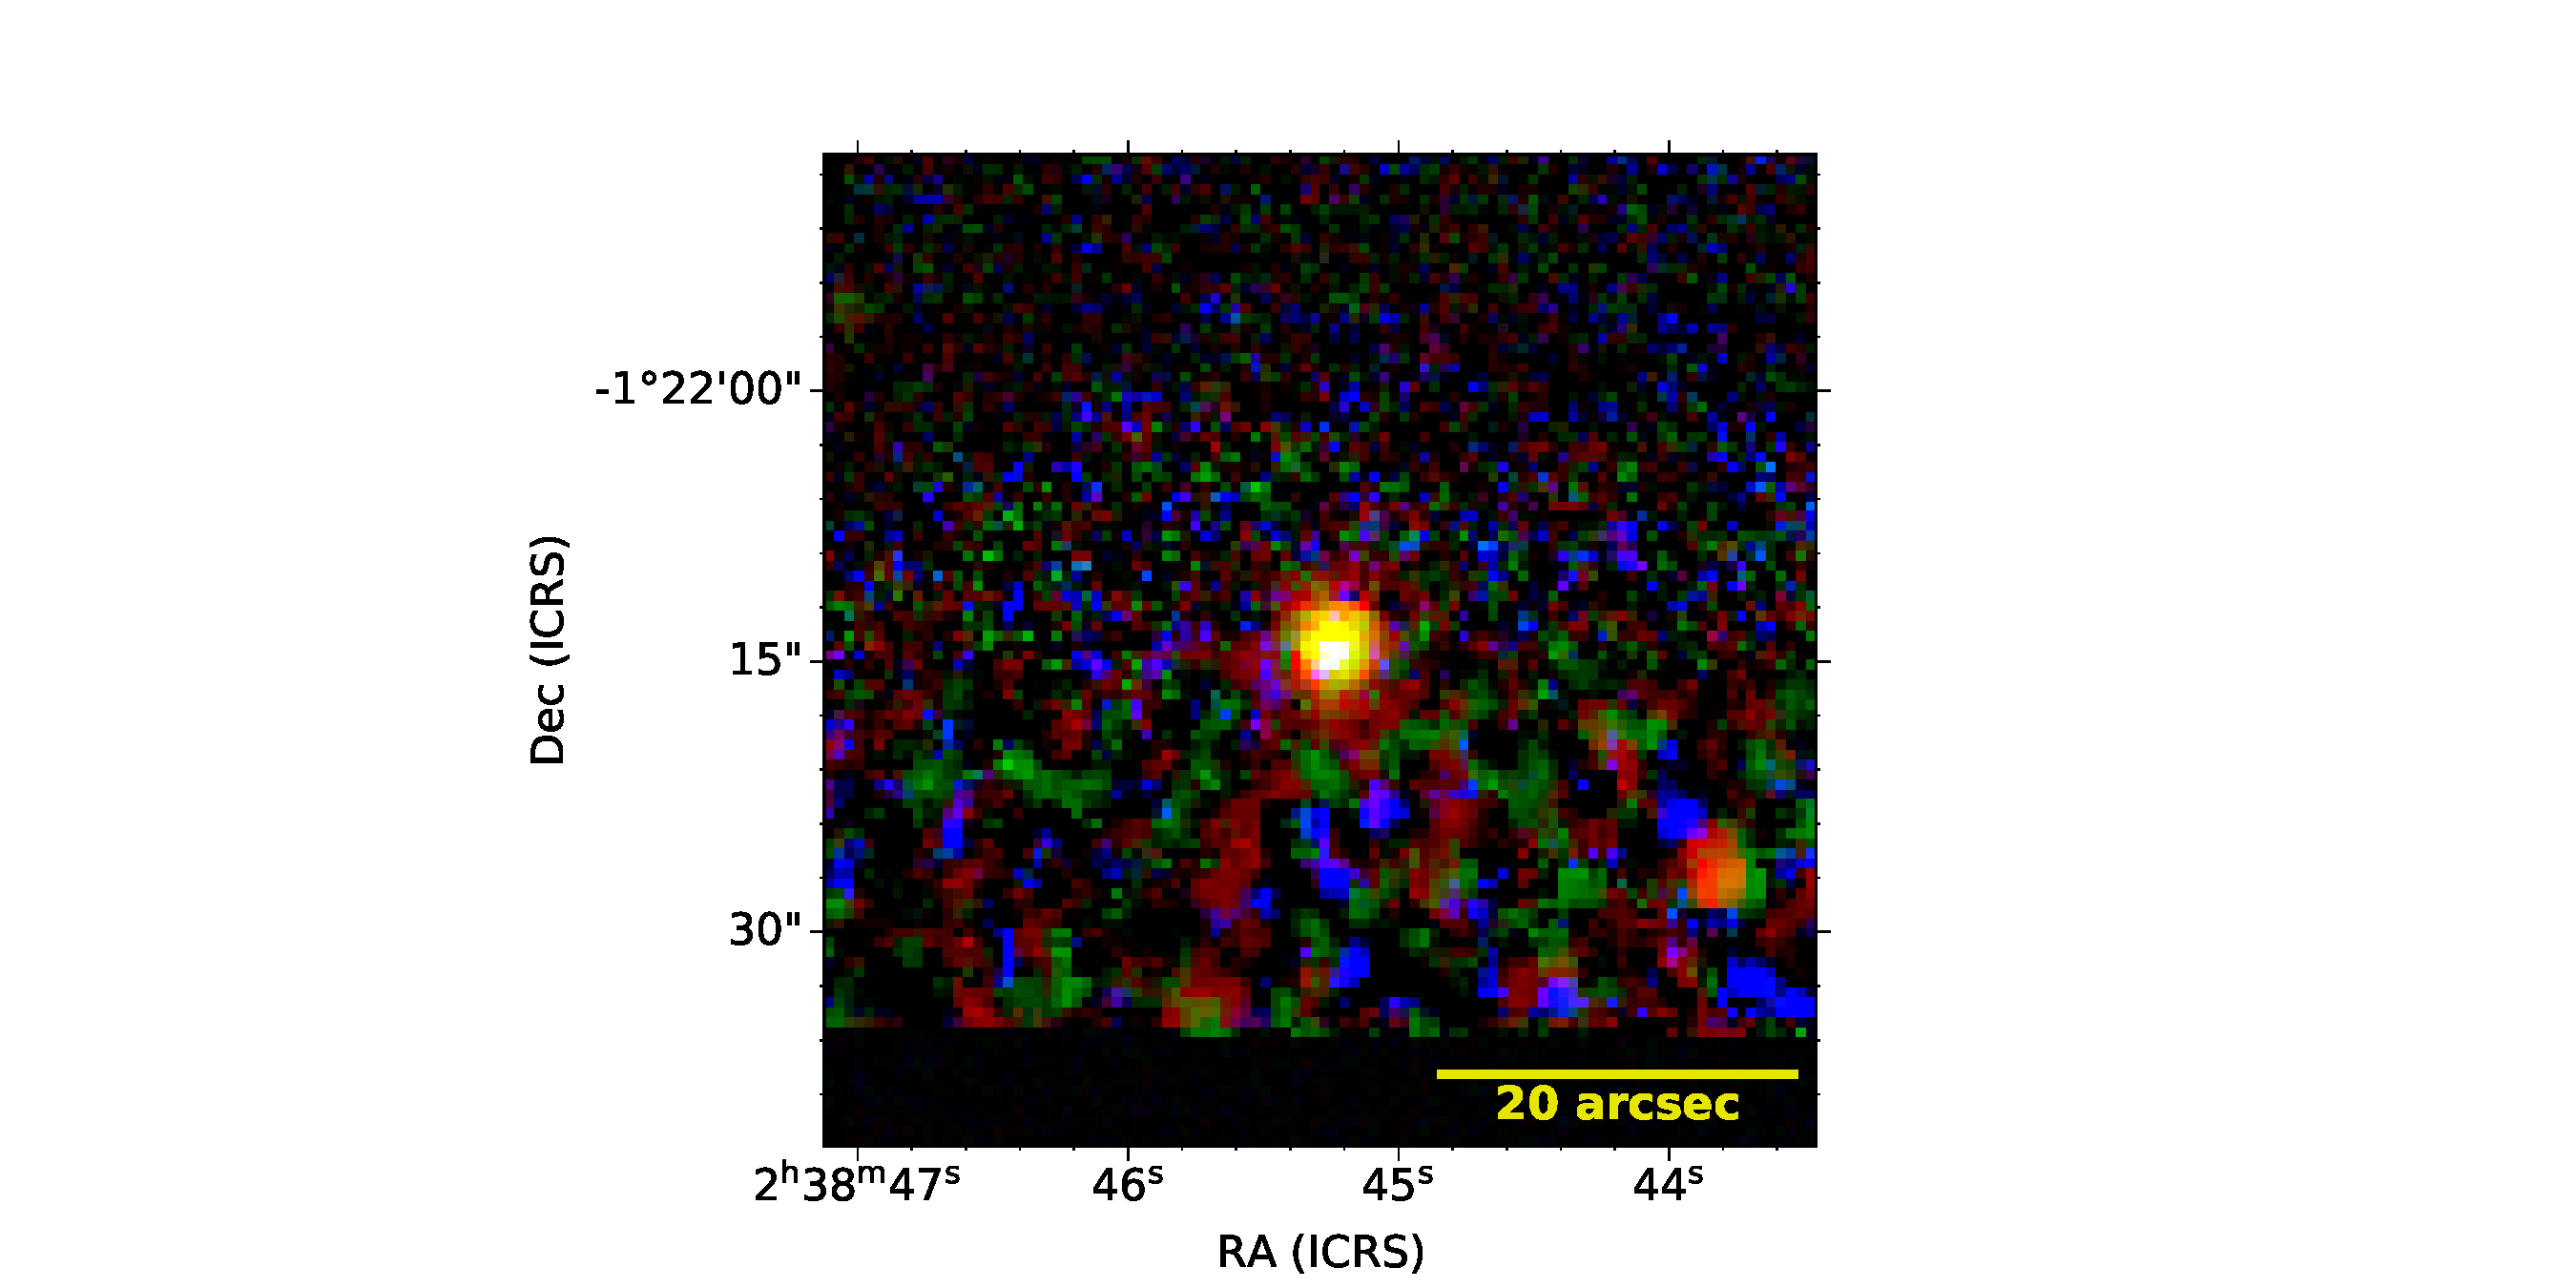
\includegraphics[width=0.4\linewidth, trim=10 0 10 20, clip]{Figs/STRIPE82-0057-001810_39-1_100_r.pdf} \\
    (c) & (d) \\
    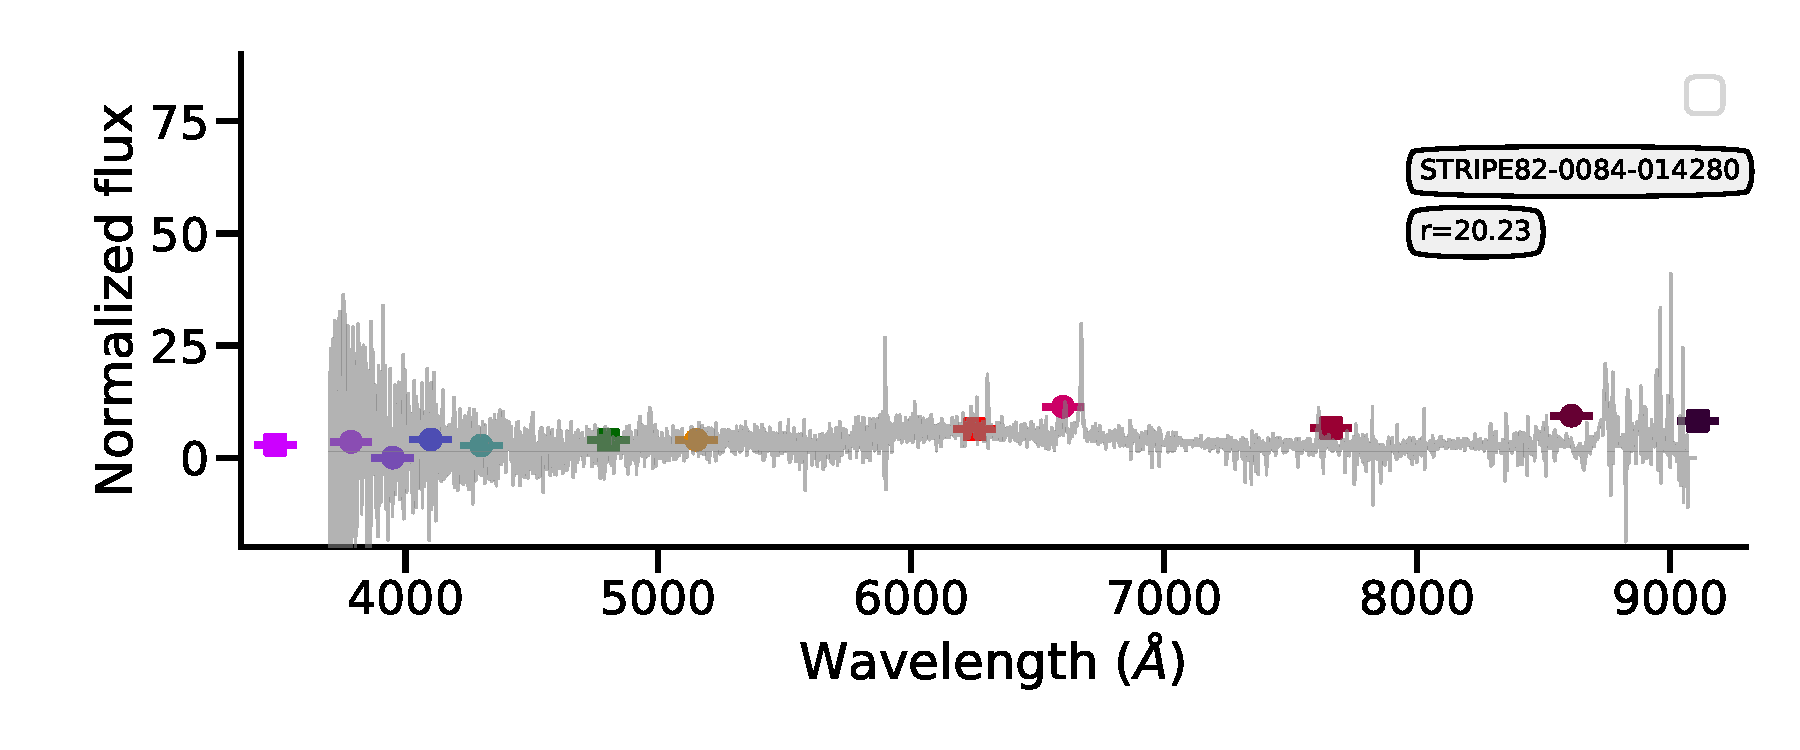
\includegraphics[trim=10 0 10 20, clip]{Figs/spec-57336-EG034838N001340M01_sp09-025-STRIPE82-0084-014280.pdf} & 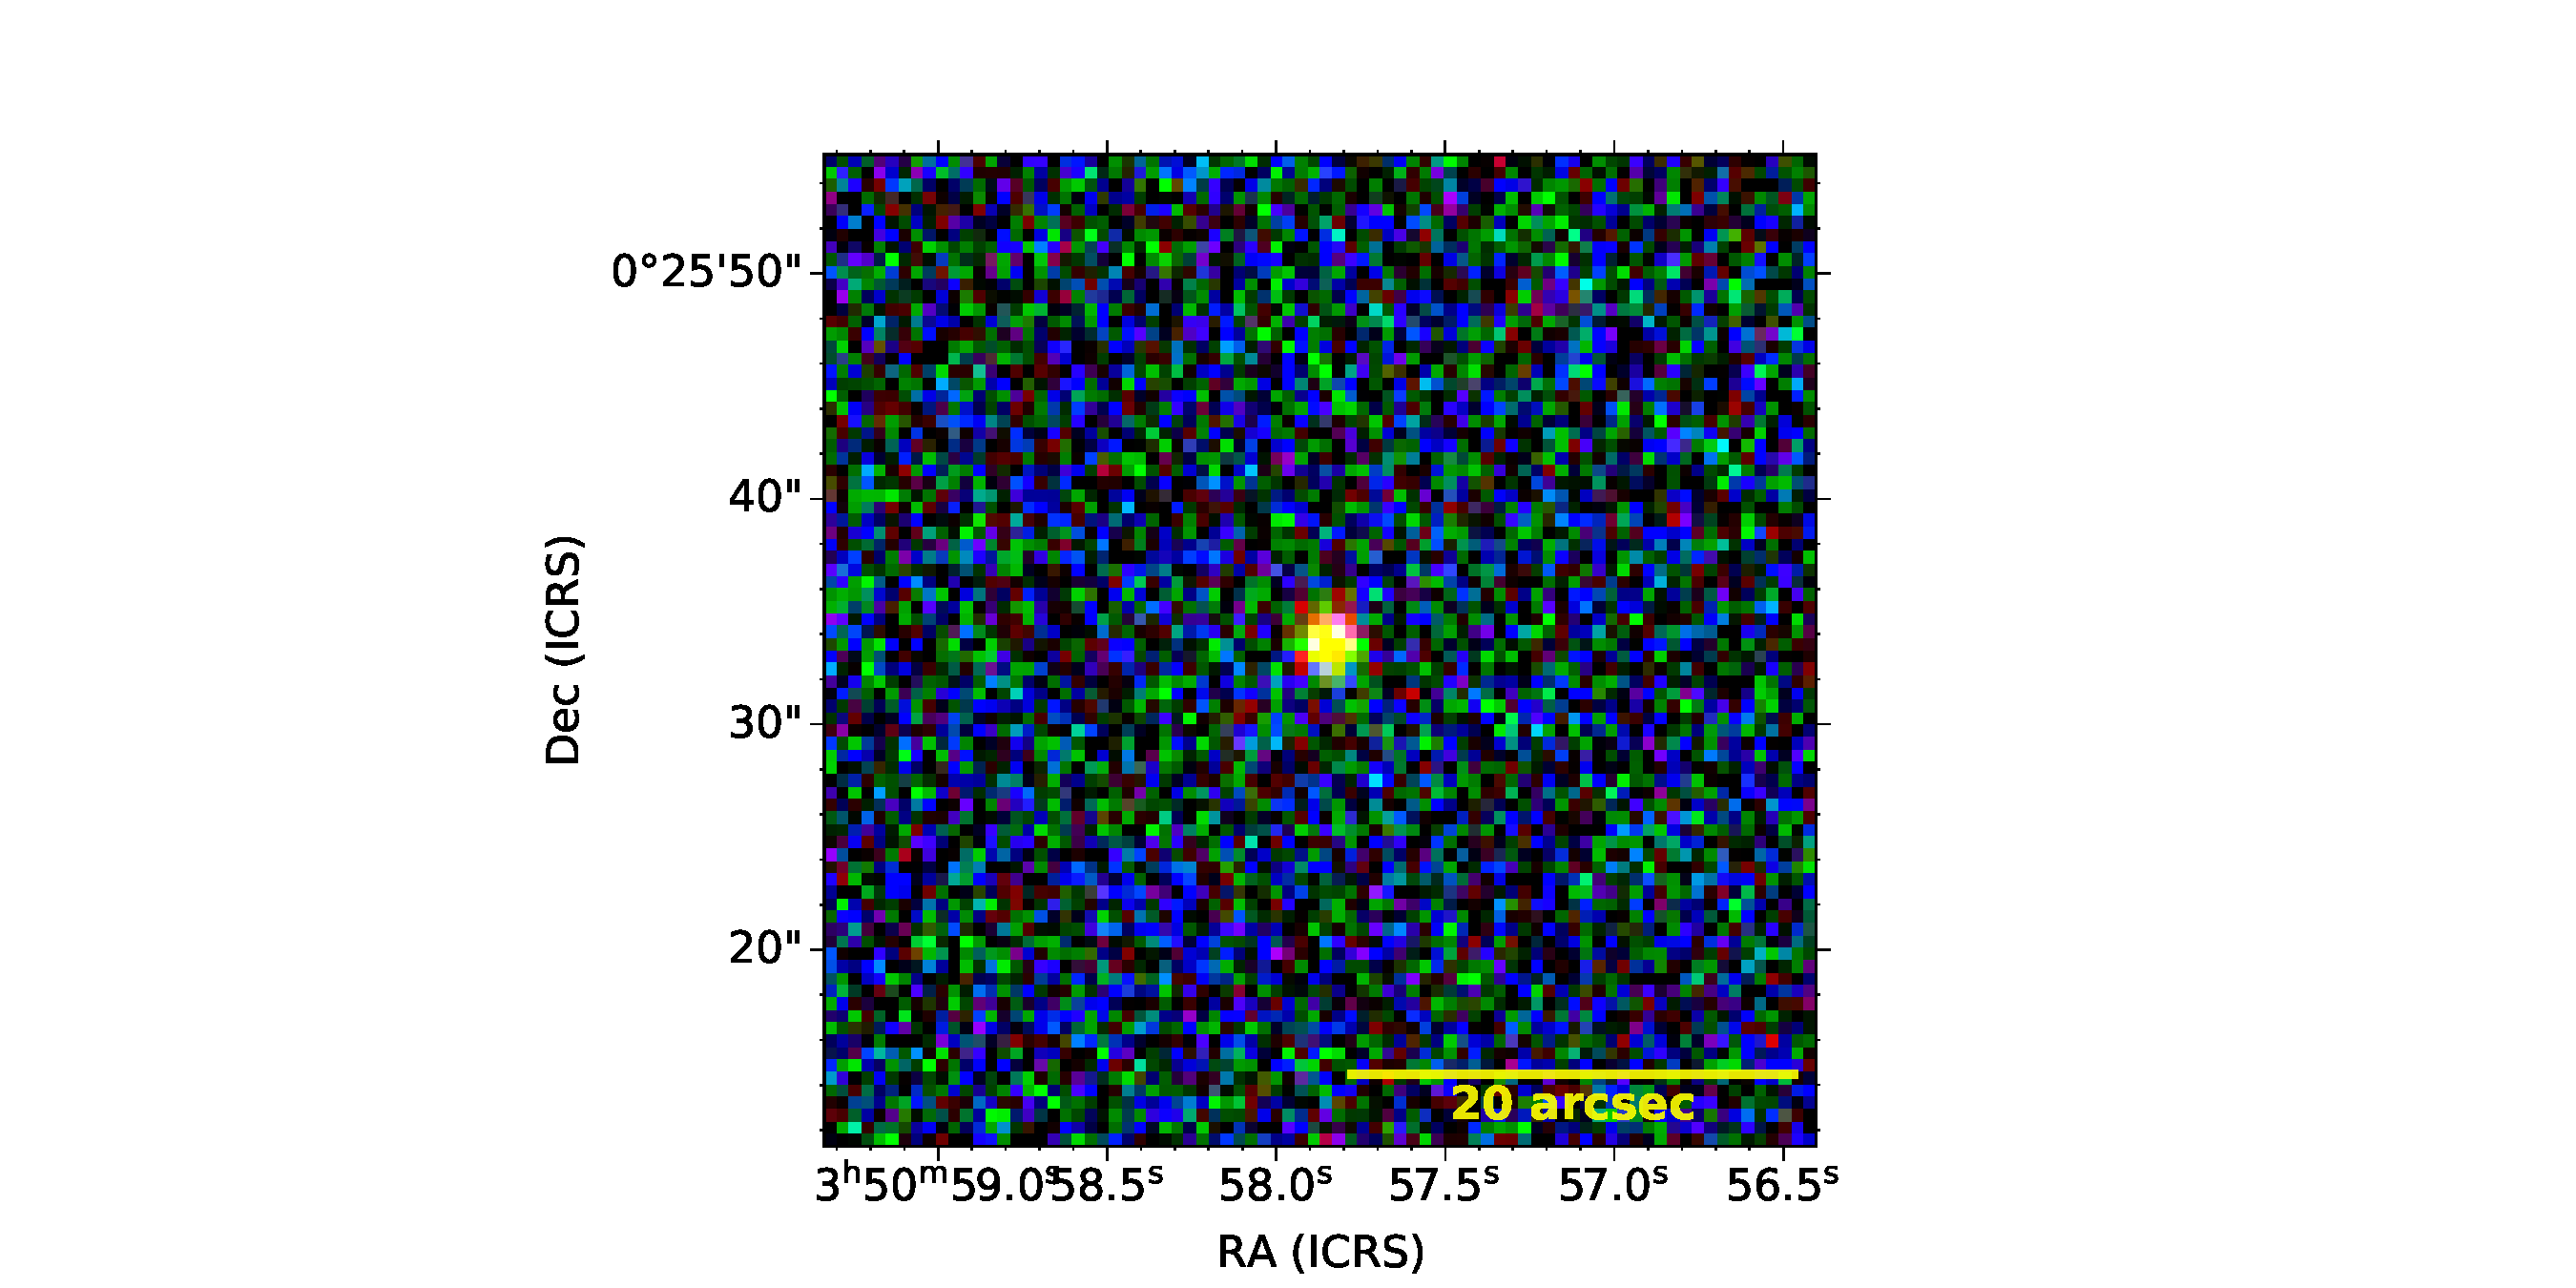
\includegraphics[width=0.4\linewidth, trim=10 0 10 20, clip]{Figs/STRIPE82-0084-014280_57-0_80_r.pdf} \\
  \end{tabular}
  \caption{Spectra of the Lamost }
  \label{fig:color-diagram}
\end{figure*}

\begin{figure*}
  \setlength\tabcolsep{0pt}
  \setkeys{Gin}{width=0.5\linewidth}
  \begin{tabular}{ll}
    (a) & (b) \\
    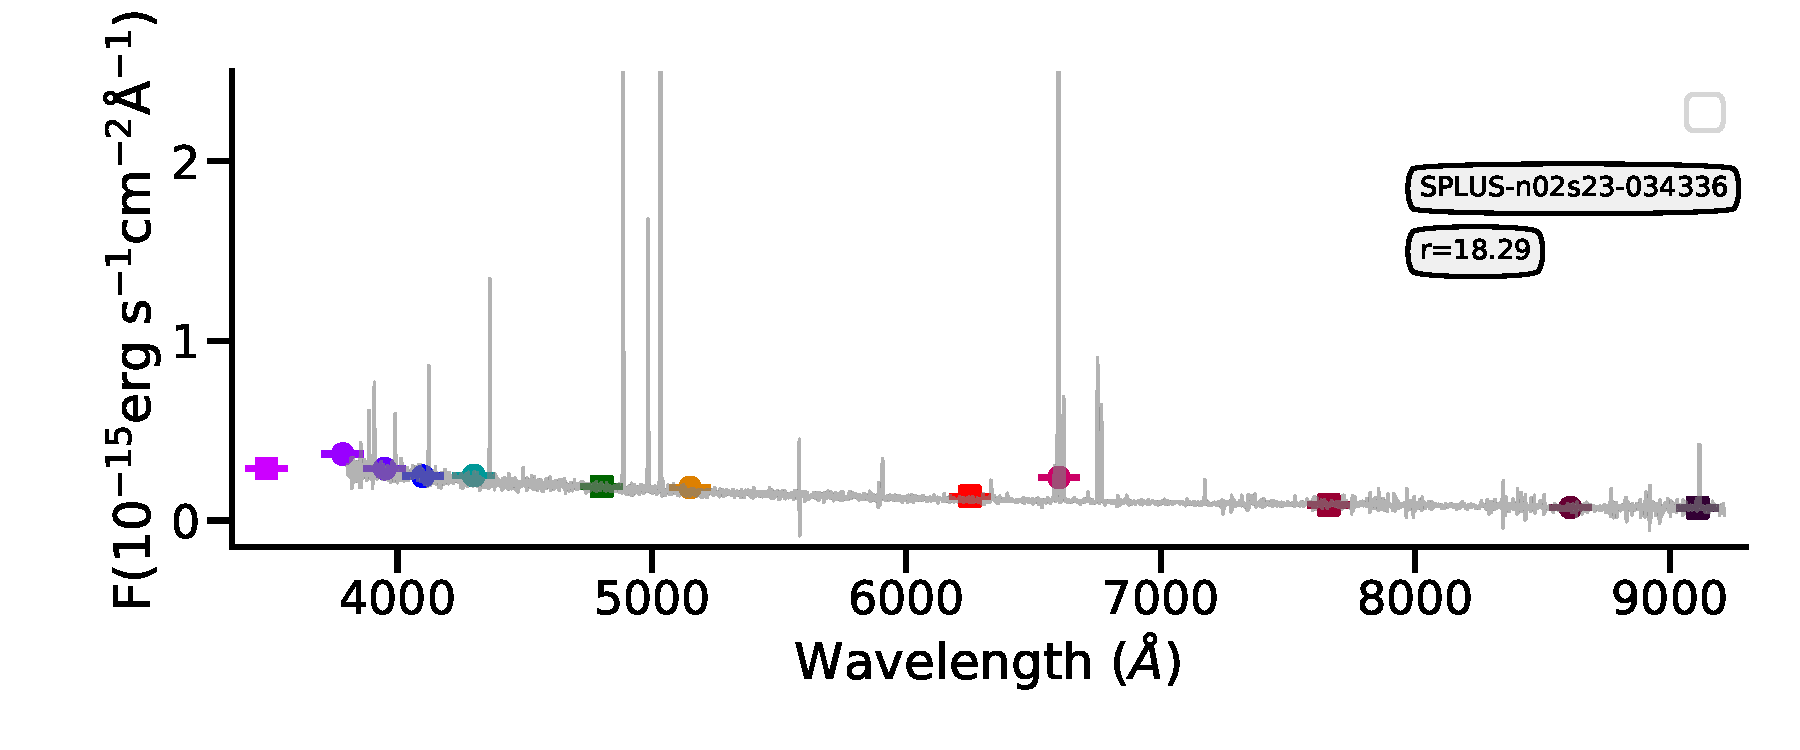
\includegraphics[trim=10 0 10 20, clip]{Figs/spec-0331-52368-0449-SPLUS-n02s23-034336.pdf} & 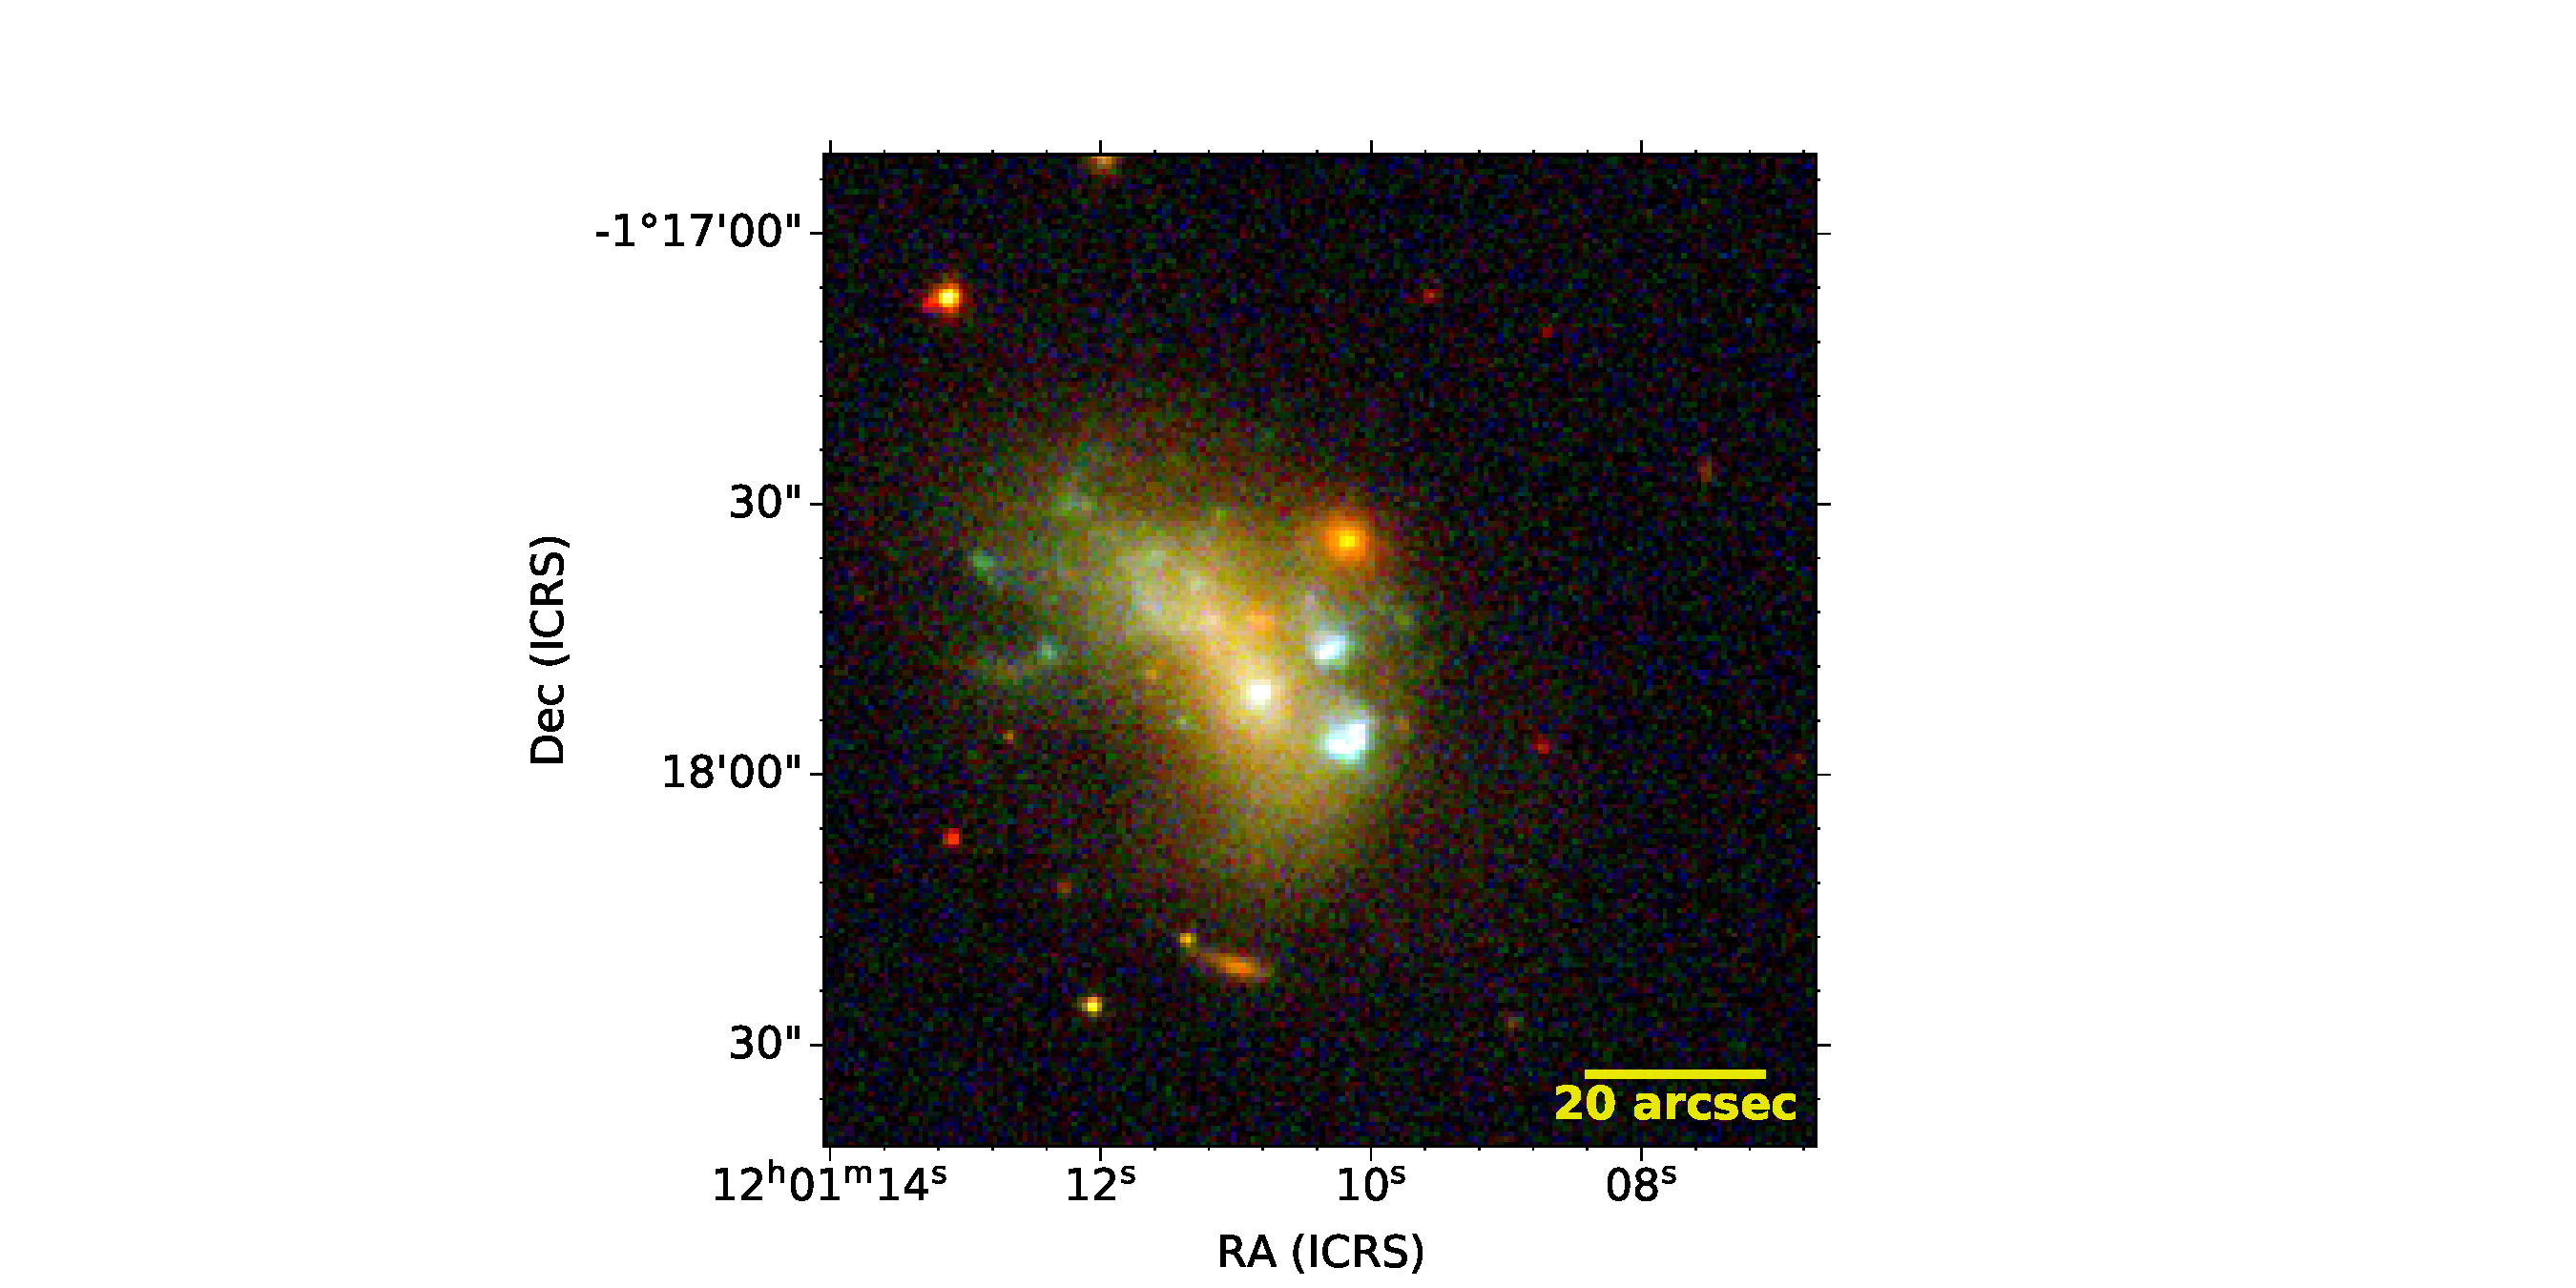
\includegraphics[width=0.4\linewidth, trim=10 0 10 20, clip]{Figs/SPLUS-n02s23-034336_180-1_200_r.pdf} \\
     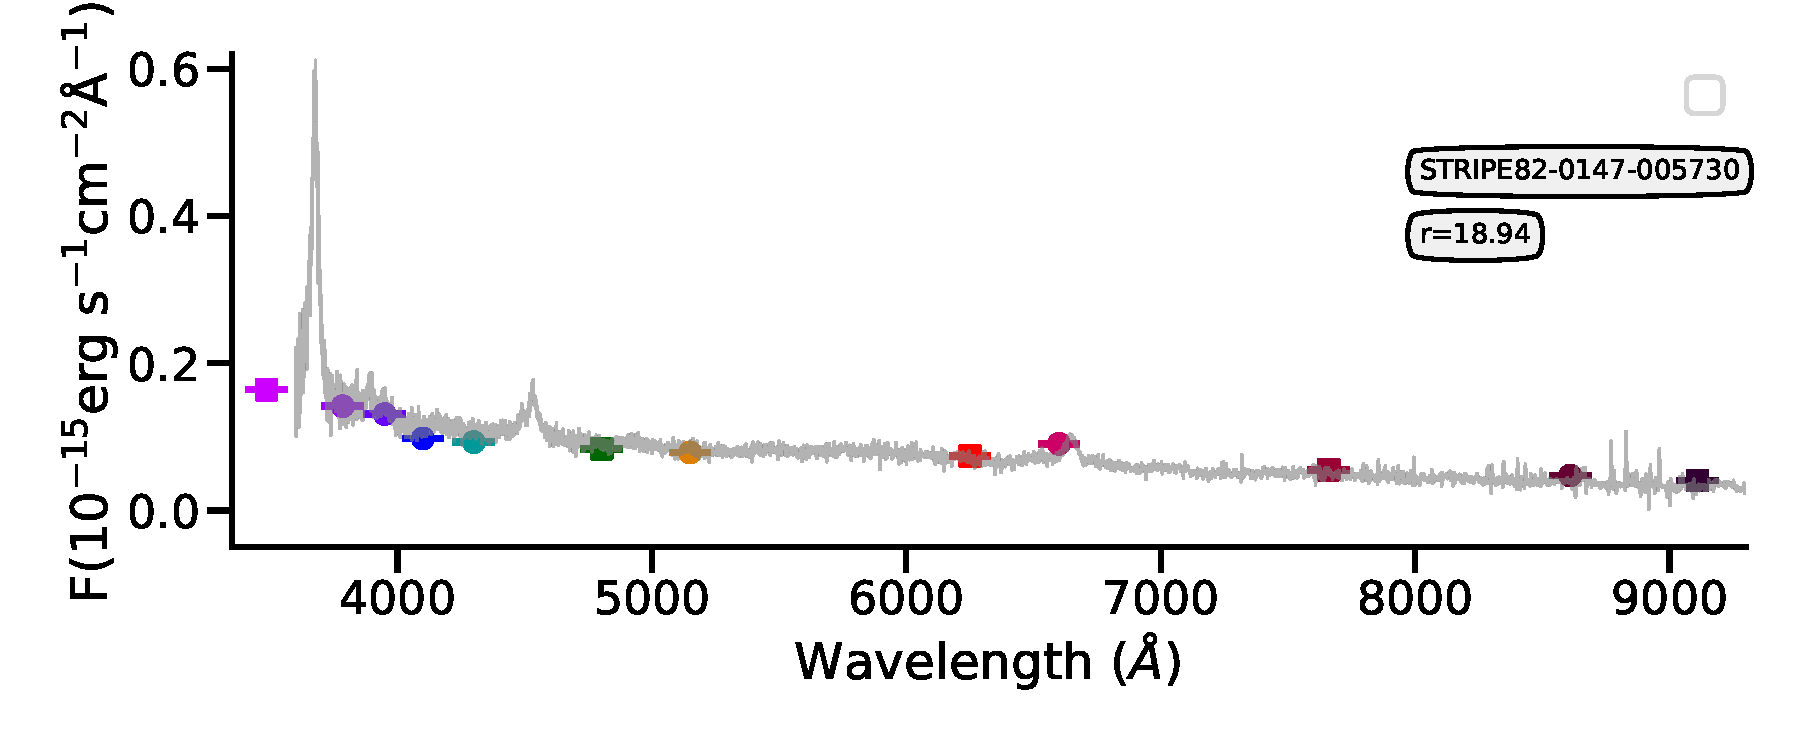
\includegraphics[trim=10 0 10 20, clip]{Figs/spec-9152-58041-0463-STRIPE82-0147-005730.pdf} & 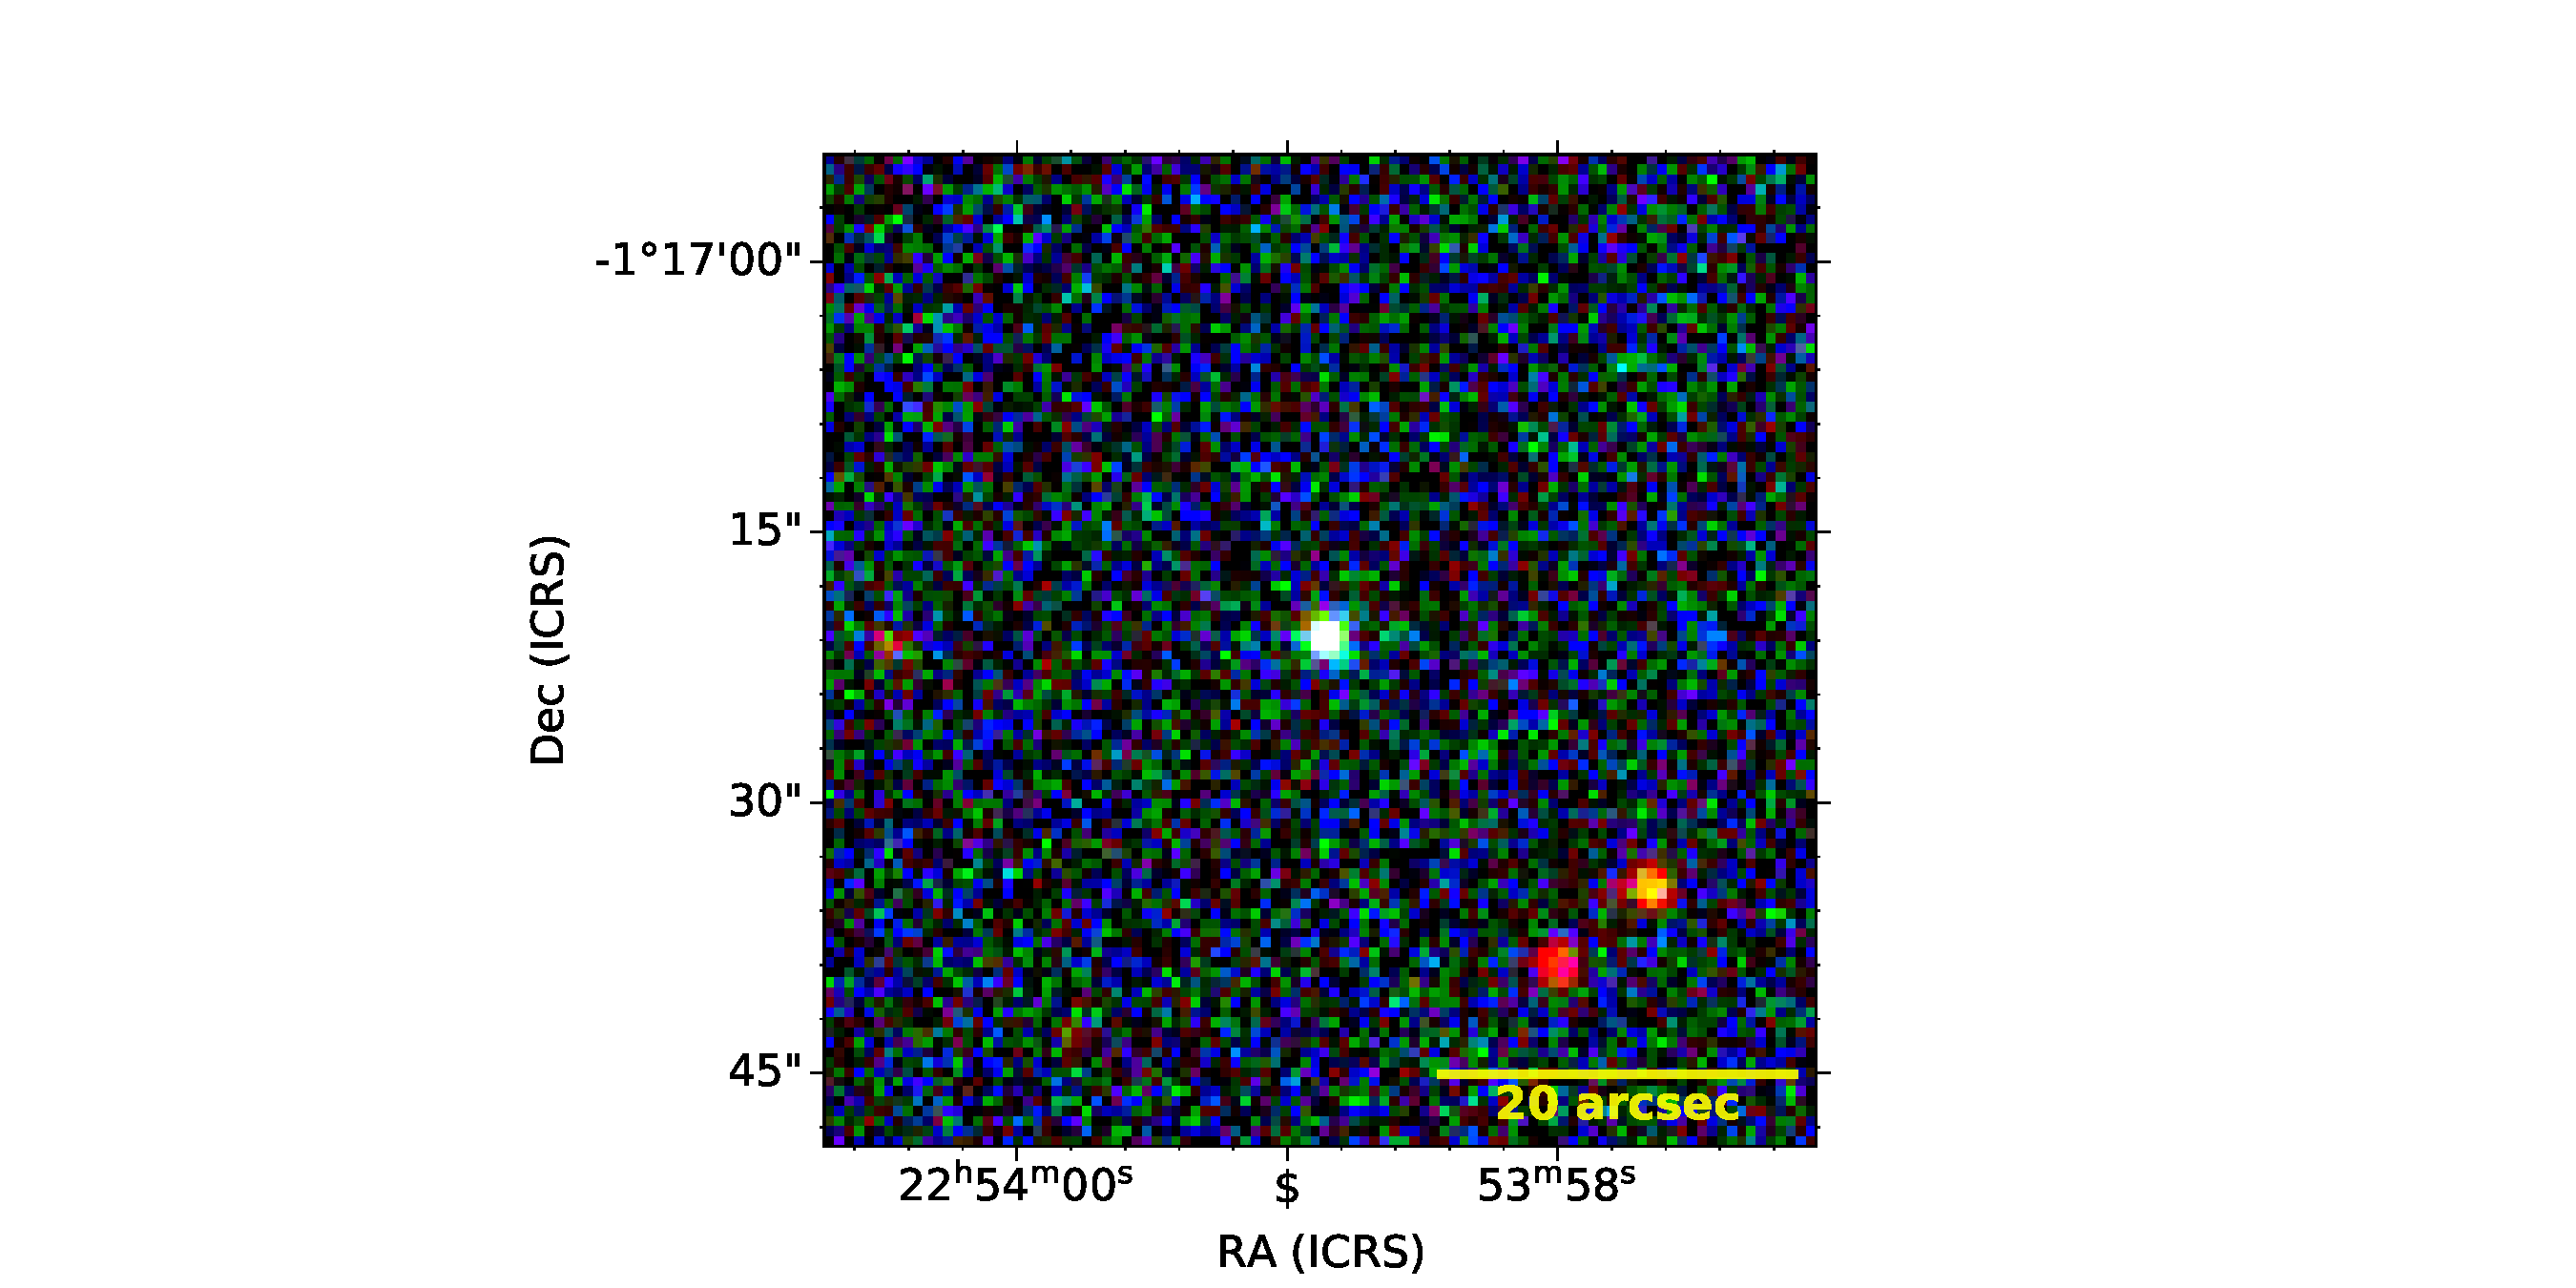
\includegraphics[width=0.4\linewidth, trim=10 0 10 20, clip]{Figs/STRIPE82-0147-005730_343-1_100_r.pdf} \\
    (c) & (d) \\
    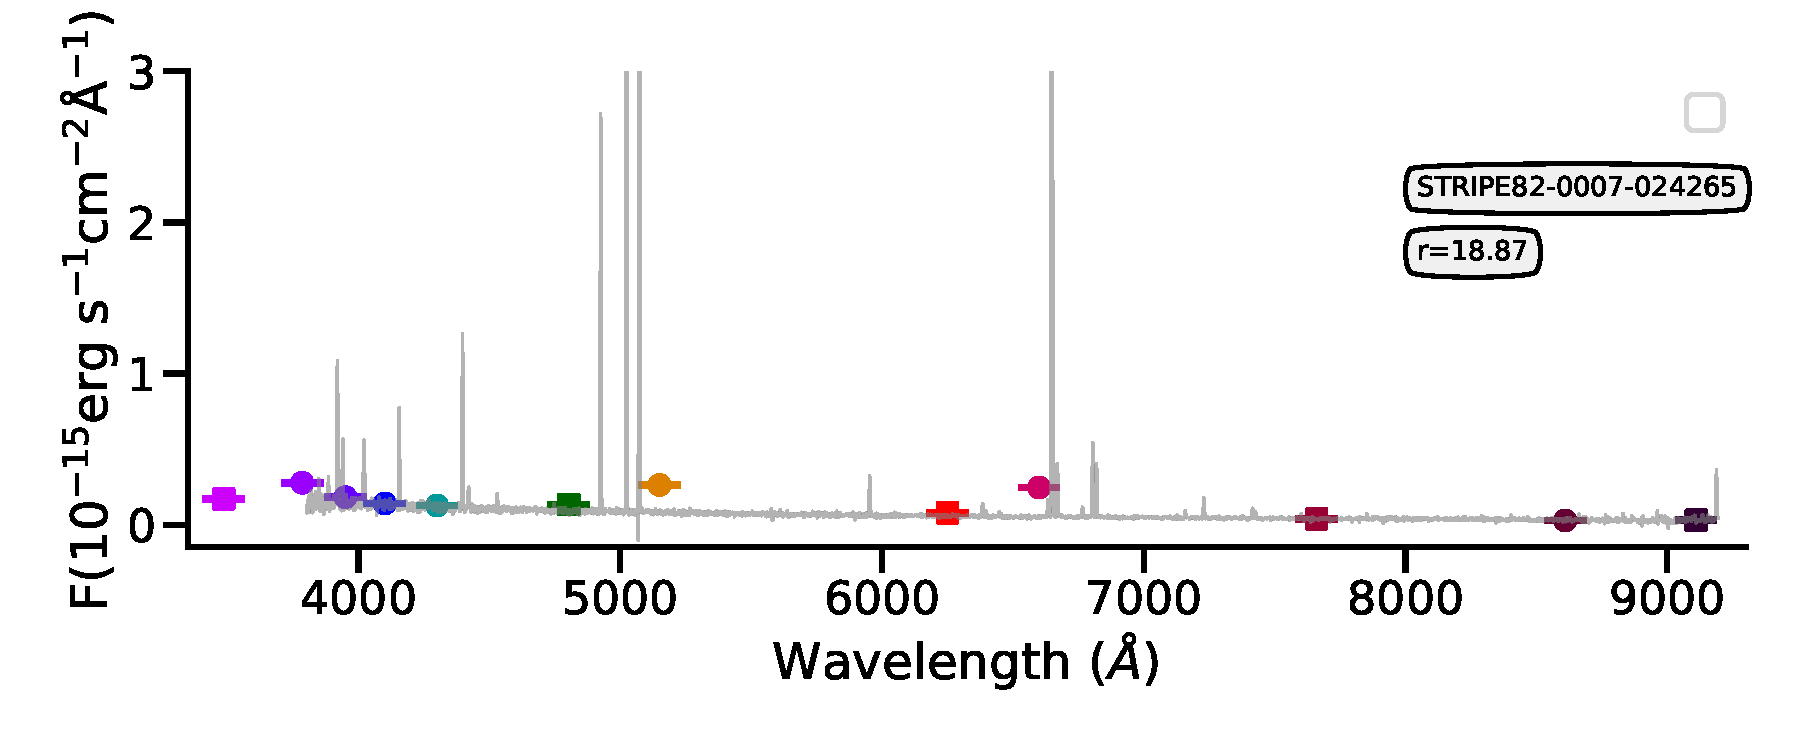
\includegraphics[trim=10 0 10 20, clip]{Figs/spec-1089-52913-0196-STRIPE82-0007-024265.pdf} & 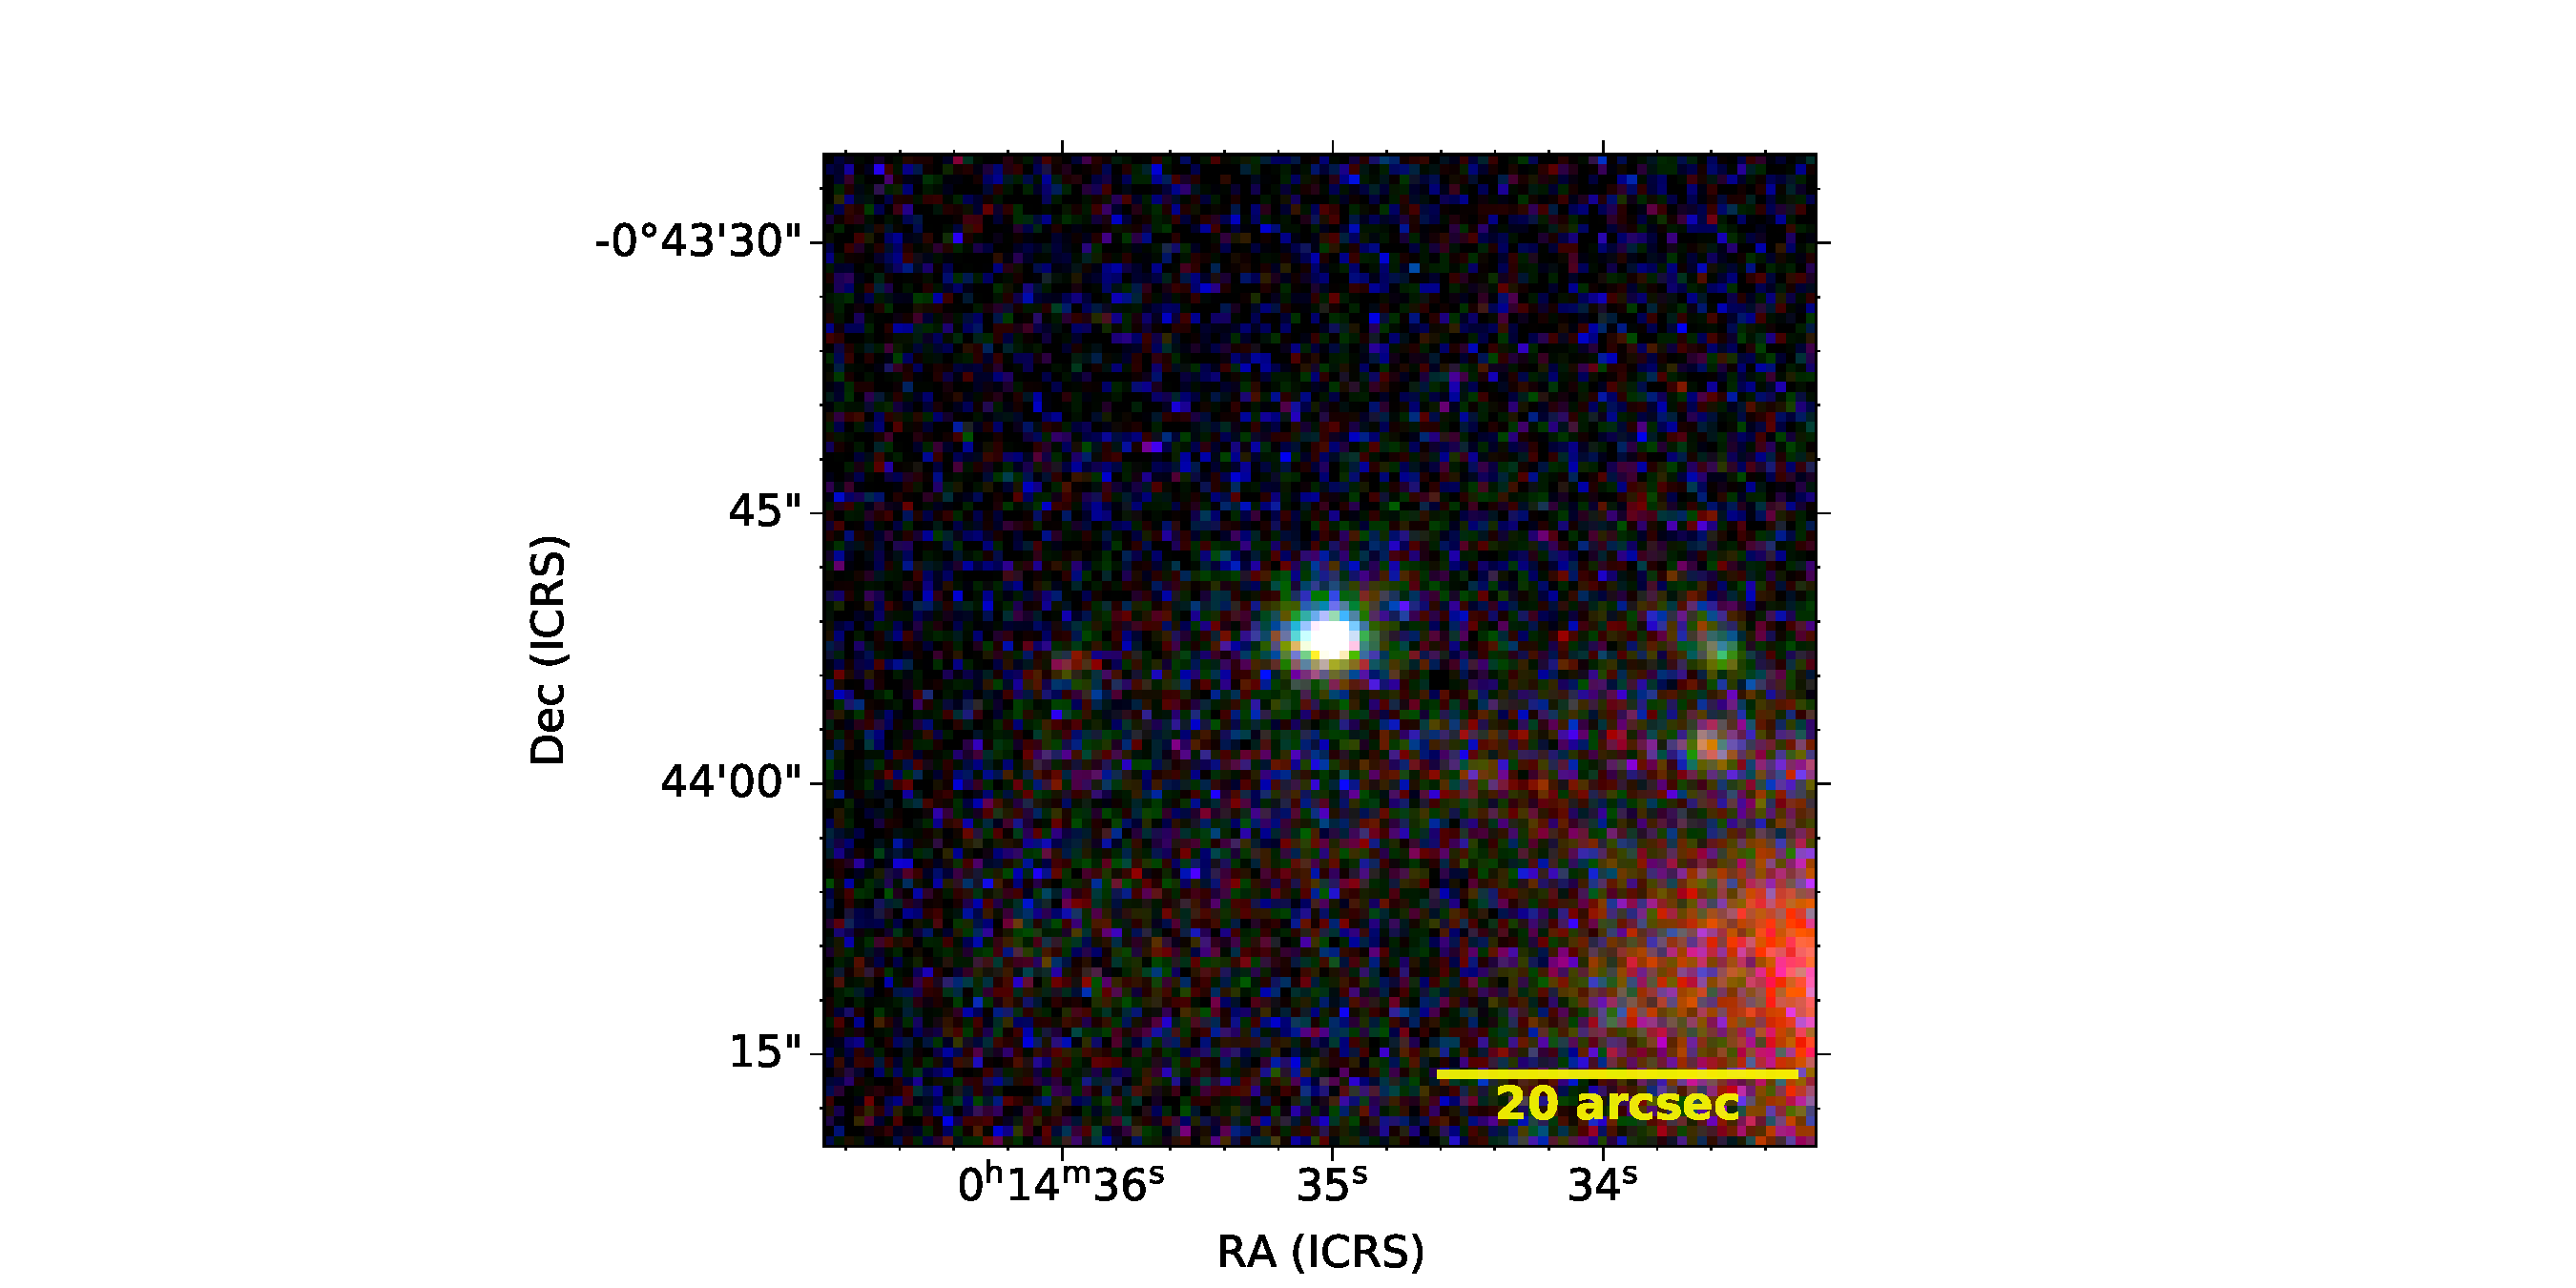
\includegraphics[width=0.4\linewidth, trim=10 0 10 20, clip]{Figs/STRIPE82-0007-024265_3-0_100_r.pdf} \\
  \end{tabular}
  \caption{Spectra of the SDSS}
  \label{fig:color-diagram}
\end{figure*}

\section{Conclusions}

We have found a important sample of emission line objects.

\section*{Acknowledgements}


%%%%%%%%%%%%%%%%%%%%%%%%%%%%%%%%%%%%%%%%%%%%%%%%%%
\section*{Data Availability}



%%%%%%%%%%%%%%%%%%%% REFERENCES %%%%%%%%%%%%%%%%%%

% The best way to enter references is to use BibTeX:

\bibliographystyle{mnras}
\bibliography{ref} % if your bibtex file is called example.bib


%%%%%%%%%%%%%%%%%%%%%%%%%%%%%%%%%%%%%%%%%%%%%%%%%%

%%%%%%%%%%%%%%%%% APPENDICES %%%%%%%%%%%%%%%%%%%%%

\appendix

\section{Some extra material}


%%%%%%%%%%%%%%%%%%%%%%%%%%%%%%%%%%%%%%%%%%%%%%%%%%


% Don't change these lines
\bsp	% typesetting comment
\label{lastpage}
\end{document}

% End of mnras_template.tex
